%&preformat-disser
\RequirePackage[l2tabu,orthodox]{nag} % Раскомментировав, можно в логе получать рекомендации 
%относительно правильного использования пакетов и предупреждения об устаревших и нерекомендуемых пакетах
% Формат А4, 14pt (ГОСТ Р 7.0.11-2011, 5.3.6)
\documentclass[a4paper,14pt,oneside,openany]{memoir}

%%%%%%%%%%%%%%%%%%%%%%%%%%%%%%%%%%%%%%%%%%%%%%%%%%%%%%
%%%% Файл упрощённых настроек шаблона диссертации %%%%
%%%%%%%%%%%%%%%%%%%%%%%%%%%%%%%%%%%%%%%%%%%%%%%%%%%%%%

%%% Инициализирование переменных, не трогать!  %%%
\newcounter{intvl}
\newcounter{otstup}
\newcounter{contnumeq}
\newcounter{contnumfig}
\newcounter{contnumtab}
\newcounter{pgnum}
\newcounter{chapstyle}
\newcounter{headingdelim}
\newcounter{headingalign}
\newcounter{headingsize}
\newcounter{tabcap}
\newcounter{tablaba}
\newcounter{tabtita}
%%%%%%%%%%%%%%%%%%%%%%%%%%%%%%%%%%%%%%%%%%%%%%%%%%%%%%

%%% Область упрощённого управления оформлением %%%

%% Интервал между заголовками и между заголовком и текстом %%
% Заголовки отделяют от текста сверху и снизу
% тремя интервалами (ГОСТ Р 7.0.11-2011, 5.3.5)
\setcounter{intvl}{2}               % Коэффициент кратности к размеру шрифта

%% Отступы у заголовков в тексте %%
\setcounter{otstup}{0}              % 0 --- без отступа; 1 --- абзацный отступ

%% Нумерация формул, таблиц и рисунков %%
% Нумерация формул
\setcounter{contnumeq}{0}   % 0 --- пораздельно (во введении подряд,
                            %       без номера раздела);
                            % 1 --- сквозная нумерация по всей диссертации
% Нумерация рисунков
\setcounter{contnumfig}{0}  % 0 --- пораздельно (во введении подряд,
                            %       без номера раздела);
                            % 1 --- сквозная нумерация по всей диссертации
% Нумерация таблиц
\setcounter{contnumtab}{1}  % 0 --- пораздельно (во введении подряд,
                            %       без номера раздела);
                            % 1 --- сквозная нумерация по всей диссертации

%% Оглавление %%
\setcounter{pgnum}{1}       % 0 --- номера страниц никак не обозначены;
                            % 1 --- Стр. над номерами страниц (дважды
                            %       компилировать после изменения настройки)
\settocdepth{subsection}    % до какого уровня подразделов выносить в оглавление
\setsecnumdepth{subsection} % до какого уровня нумеровать подразделы


%% Текст и форматирование заголовков %%
\setcounter{chapstyle}{1}     % 0 --- разделы только под номером;
                              % 1 --- разделы с названием "Глава" перед номером
\setcounter{headingdelim}{1}  % 0 --- номер отделен пропуском в 1em или \quad;
                              % 1 --- номера разделов и приложений отделены
                              %       точкой с пробелом, подразделы пропуском
                              %       без точки;
                              % 2 --- номера разделов, подразделов и приложений
                              %       отделены точкой с пробелом.

%% Выравнивание заголовков в тексте %%
\setcounter{headingalign}{0}  % 0 --- по центру;
                              % 1 --- по левому краю

%% Размеры заголовков в тексте %%
\setcounter{headingsize}{0}   % 0 --- по ГОСТ, все всегда 14 пт;
                              % 1 --- пропорционально изменяющийся размер
                              %       в зависимости от базового шрифта

%% Подпись таблиц %%
\setcounter{tabcap}{0}  % 0 --- по ГОСТ, номер таблицы и название разделены
                        %       тире, выровнены по левому краю, при
                        %       необходимостина нескольких строках;
                        % 1 --- подпись таблицы не по ГОСТ, на двух и более
                        %       строках, дальнейшие настройки:
%Выравнивание первой строки, с подписью и номером
\setcounter{tablaba}{2} % 0 --- по левому краю;
                        % 1 --- по центру;
                        % 2 --- по правому краю
%Выравнивание строк с самим названием таблицы
\setcounter{tabtita}{1} % 0 --- по левому краю;
                        % 1 --- по центру;
                        % 2 --- по правому краю
%Разделитель записи «Таблица #» и названия таблицы
\newcommand{\tablabelsep}{ }

%% Подпись рисунков %%
%Разделитель записи «Рисунок #» и названия рисунка
\newcommand{\figlabelsep}{~\cyrdash\ }  % (ГОСТ 2.105, 4.3.1)
                                        % "--- здесь не работает

%%% Цвета гиперссылок %%%
% Latex color definitions: http://latexcolor.com/
\definecolor{linkcolor}{rgb}{0.9,0,0}
\definecolor{citecolor}{rgb}{0,0.6,0}
\definecolor{urlcolor}{rgb}{0,0,1}
%\definecolor{linkcolor}{rgb}{0,0,0} %black
%\definecolor{citecolor}{rgb}{0,0,0} %black
%\definecolor{urlcolor}{rgb}{0,0,0} %black
            % общие настройки шаблона
%%% Проверка используемого TeX-движка %%%
\newif\ifxetexorluatex   % определяем новый условный оператор (http://tex.stackexchange.com/a/47579)
\ifxetex
    \xetexorluatextrue
\else
    \ifluatex
        \xetexorluatextrue
    \else
        \xetexorluatexfalse
    \fi
\fi

\newif\ifsynopsis           % Условие, проверяющее, что документ --- автореферат

\usepackage{etoolbox}[2015/08/02]               % Для продвинутой проверки разных условий
\providebool{presentation}

%%% Поля и разметка страницы %%%
\usepackage{pdflscape}                              % Для включения альбомных страниц
\usepackage{geometry}                               % Для последующего задания полей

%%% Математические пакеты %%%
\usepackage{amsthm,amsmath,amscd}   % Математические дополнения от AMS
\usepackage{amsfonts,amssymb}       % Математические дополнения от AMS
\usepackage{mathtools}              % Добавляет окружение multlined
\usepackage{xfrac}                  % Красивые дроби
\usepackage[
    locale = DE,
    list-separator       = {;\,},
    list-final-separator = {;\,},
    list-pair-separator  = {;\,},
    range-phrase={\text{\ensuremath{-}}},
    % quotient-mode        = fraction, % красивые дроби могут не соответствовать ГОСТ
    fraction-function    = \sfrac,
    separate-uncertainty,
    ]{siunitx}                      % Размерности SI
\sisetup{inter-unit-product = \ensuremath{{}\cdot{}}}

% Кириллица в нумерации subequations
% Для правильной работы требуется выполнение сразу после загрузки пакетов
\patchcmd{\subequations}{\def\theequation{\theparentequation\alph{equation}}}
{\def\theequation{\theparentequation\asbuk{equation}}}
{\typeout{subequations patched}}{\typeout{subequations not patched}}

%%%% Установки для размера шрифта 14 pt %%%%
%% Формирование переменных и констант для сравнения (один раз для всех подключаемых файлов)%%
%% должно располагаться до вызова пакета fontspec или polyglossia, потому что они сбивают его работу
\newlength{\curtextsize}
\newlength{\bigtextsize}
\setlength{\bigtextsize}{13.9pt}

\makeatletter
%\show\f@size                                       % неплохо для отслеживания, но вызывает стопорение процесса, если документ компилируется без команды  -interaction=nonstopmode
\setlength{\curtextsize}{\f@size pt}
\makeatother

%%% Кодировки и шрифты %%%
\ifxetexorluatex
    \PassOptionsToPackage{no-math}{fontspec}        % https://tex.stackexchange.com/a/26295/104425
    \usepackage{polyglossia}[2014/05/21]            % Поддержка многоязычности (fontspec подгружается автоматически)
\else
   %%% Решение проблемы копирования текста в буфер кракозябрами
    \ifnumequal{\value{usealtfont}}{0}{}{
        \input glyphtounicode.tex
        \input glyphtounicode-cmr.tex %from pdfx package
        \pdfgentounicode=1
    }
    \usepackage{cmap}                               % Улучшенный поиск русских слов в полученном pdf-файле
    \ifnumequal{\value{usealtfont}}{2}{}{
        \defaulthyphenchar=127                      % Если стоит до fontenc, то переносы не впишутся в выделяемый текст при копировании его в буфер обмена
    }
    \usepackage{textcomp}
    \usepackage[T1,T2A]{fontenc}                    % Поддержка русских букв
    \ifnumequal{\value{usealtfont}}{1}{% Используется pscyr, при наличии
        \IfFileExists{pscyr.sty}{\usepackage{pscyr}}{}  % Подключение pscyr
    }{}
    \usepackage[utf8]{inputenc}[2014/04/30]         % Кодировка utf8
    \usepackage[english, russian]{babel}[2014/03/24]% Языки: русский, английский
    \makeatletter\AtBeginDocument{\let\@elt\relax}\makeatother % babel 3.40 fix
    \ifnumequal{\value{usealtfont}}{2}{
        % http://dxdy.ru/post1238763.html#p1238763
        \usepackage[scaled=0.960]{XCharter}[2017/12/19] % Подключение русифицированных шрифтов XCharter
        \usepackage[charter, vvarbb, scaled=1.048]{newtxmath}[2017/12/14]
        \ifpresentation
        \else
            \setDisplayskipStretch{-0.078}
        \fi
    }{}
\fi

%%% Оформление абзацев %%%
\usepackage{indentfirst}                            % Красная строка

%%% Цвета %%%
\ifpresentation
\else
    \usepackage[dvipsnames, table, hyperref]{xcolor} % Совместимо с tikz
\fi

%%% Таблицы %%%
\usepackage{longtable,ltcaption} % Длинные таблицы
\usepackage{multirow,makecell}   % Улучшенное форматирование таблиц
\usepackage{tabu, tabulary}      % таблицы с автоматически подбирающейся
                                 % шириной столбцов (tabu обязательно
                                 % до hyperref вызывать)
\usepackage{threeparttable}      % автоматический подгон ширины подписи таблицы

%%% Общее форматирование
\usepackage{soulutf8}                               % Поддержка переносоустойчивых подчёркиваний и зачёркиваний
\usepackage{icomma}                                 % Запятая в десятичных дробях

%%% Оптимизация расстановки переносов и длины последней строки абзаца
\IfFileExists{impnattypo.sty}{% проверка установленности пакета impnattypo
    \ifluatex
        \ifnumequal{\value{draft}}{1}{% Черновик
            \usepackage[hyphenation, lastparline, nosingleletter, homeoarchy,
            rivers, draft]{impnattypo}
        }{% Чистовик
            \usepackage[hyphenation, lastparline, nosingleletter]{impnattypo}
        }
    \else
        \usepackage[hyphenation, lastparline]{impnattypo}
    \fi
}{}

%% Векторная графика

\usepackage{tikz}                   % Продвинутый пакет векторной графики
\usetikzlibrary{chains}             % Для примера tikz рисунка
\usetikzlibrary{shapes.geometric}   % Для примера tikz рисунка
\usetikzlibrary{shapes.symbols}     % Для примера tikz рисунка
\usetikzlibrary{arrows}             % Для примера tikz рисунка
\usetikzlibrary{plotmarks}

\usepackage{pgfplots}
\usepgfplotslibrary{ternary}

%%% Гиперссылки %%%
\usepackage{hyperref}[2012/11/06]

%%% Изображения %%%
\usepackage{graphicx}[2014/04/25]                   % Подключаем пакет работы с графикой

%%% Счётчики %%%
\usepackage[figure,table]{totalcount}               % Счётчик рисунков и таблиц
\usepackage{totcount}                               % Пакет создания счётчиков на основе последнего номера подсчитываемого элемента (может требовать дважды компилировать документ)
\usepackage{totpages}                               % Счётчик страниц, совместимый с hyperref (ссылается на номер последней страницы). Желательно ставить последним пакетом в преамбуле

%%% Продвинутое управление групповыми ссылками (пока только формулами) %%%
\ifpresentation
\else
    \usepackage[russian]{cleveref} % cleveref имеет сложности со считыванием
    % языка из babel. Такое решение русификации вывода выбрано вместо
    % определения в documentclass из опасности что-то лишнее передать во все
    % остальные пакеты, включая библиографию.
    \creflabelformat{equation}{#2#1#3} % Формат по умолчанию ставил круглые
    % скобки вокруг каждого номера ссылки, теперь просто номера ссылок без
    % какого-либо дополнительного оформления
    \crefrangelabelformat{equation}{#3#1#4\cyrdash#5#2#6} % Интервалы в русском
    % языке принято делать через тире, если иное не оговорено

    % решение проблемы с "и" в \labelcref
    % https://tex.stackexchange.com/a/455124/104425
    \ifxetexorluatex
        \DeclareTextSymbol{\cyri}\UnicodeEncodingName{"0438} % и
    \fi

    % Добавление возможности использования пробелов в \labelcref
    % https://tex.stackexchange.com/a/340502/104425
    \usepackage{kvsetkeys}
    \makeatletter
    \let\org@@cref\@cref
    \renewcommand*{\@cref}[2]{%
        \edef\process@me{%
            \noexpand\org@@cref{#1}{\zap@space#2 \@empty}%
        }\process@me
    }
    \makeatother

    \newcommand{\eqrefs}[1]{(\labelcref{#1})}
    \newcommand{\refs}[1]{\labelcref{#1}}
\fi

\ifnumequal{\value{draft}}{1}{% Черновик
    \usepackage[firstpage]{draftwatermark}
    \SetWatermarkText{DRAFT}
    \SetWatermarkFontSize{14pt}
    \SetWatermarkScale{15}
    \SetWatermarkAngle{45}
}{}

%%% Исправление положения якорей подписей (под)рисунков %%%
% Без hypcap и патча, при клике по ссылке на подрисунок, просмотрщик pdf прыгает "к подписи" а не "к рисунку".
% Подробнее: https://github.com/AndreyAkinshin/Russian-Phd-LaTeX-Dissertation-Template/issues/238
% (!) Даже с патчем, если мешать в одной фиге разные типы подфиг (subbottom и subcaption) - ссылки всё равно будут работать неправильно  (см. https://www.overleaf.com/read/czmbmmtnqrrg ).
\ifpresentation
\else
    \usepackage[all]{hypcap}

    \makeatletter
    \ltx@ifclasslater{memoir}{2018/12/13}{
        % Предполагается, что в следующей версии класс будет исправлен
        \typeout{Assuming this version of memoir is free from the jumping-to-caption bug.}
    }{
        \usepackage{xpatch}

        \newcommand\mem@step@subcounter{\refstepcounter{sub\@captype}\@contkeep}

        \xpatchcmd{\@memsubbody}%
        {\refstepcounter{sub\@captype}\@contkeep}% search pattern
        {}% replacement
        {\typeout{@memsubbody is patched}}%
        {\typeout{@memsubbody is NOT patched}}%

        \xpatchcmd{\@memcontsubbody}%
        {\refstepcounter{sub\@captype}\@contkeep}% pattern
        {}% replacement
        {\typeout{@memcontsubbody is patched}}%
        {\typeout{@memcontsubbody is NOT patched}}%

        \xpatchcmd{\@memsubfloat}%
        {\vbox\bgroup}% search pattern
        {\vbox\bgroup\mem@step@subcounter}% replacement
        {\typeout{@memsubfloat patch is ok}}%
        {\typeout{@memsubfloat patch is NOT ok}}%

        \xpatchcmd{\subcaption}%
        {\refstepcounter{sub\@captype}}% search pattern
        {\H@refstepcounter{sub\@captype}}% replacement
        {\typeout{subcaption second patch is ok}}%
        {\typeout{subcaption second patch is NOT ok}}%
    }
    \makeatother
\fi

%%% Цитата, не приводимая в автореферате:
% возможно, актуальна только для biblatex
%\newcommand{\citeinsynopsis}[1]{\ifsynopsis\else ~\cite{#1} \fi}

% если текущий процесс запущен библиотекой tikz-external, то прекомпиляция должна быть включена
\ifdefined\tikzexternalrealjob
    \setcounter{imgprecompile}{1}
\fi

\ifnumequal{\value{imgprecompile}}{1}{% Только если у нас включена предкомпиляция
    \usetikzlibrary{external}   % подключение возможности предкомпиляции
    \tikzexternalize[prefix=images/cache/] % activate! % здесь можно указать отдельную папку для скомпилированных файлов
    \ifxetex
        \tikzset{external/up to date check={diff}}
    \fi
}{}
         % Пакеты общие для диссертации и автореферата
\synopsisfalse                      % Этот документ --- не автореферат
\input{Dissertation/dispackages}    % Пакеты для диссертации
\usepackage{fr-longtable}    %ради \endlasthead

% Листинги с исходным кодом программ
\usepackage{fancyvrb}
\usepackage{listings}
\lccode`\~=0\relax %Без этого хака из-за особенностей пакета listings перестают работать конструкции с \MakeLowercase и т. п. в (xe|lua)latex

% Русская традиция начертания греческих букв
\usepackage{upgreek} % прямые греческие ради русской традиции

\usepackage{rotating}

%%% Микротипографика
%\ifnumequal{\value{draft}}{0}{% Только если у нас режим чистовика
%    \usepackage[final, babel, shrink=45]{microtype}[2016/05/14] % улучшает представление букв и слов в строках, может помочь при наличии отдельно висящих слов
%}{}

% Отметка о версии черновика на каждой странице
% Чтобы работало надо в своей локальной копии по инструкции
% https://www.ctan.org/pkg/gitinfo2 создать небходимые файлы в папке
% ./git/hooks
% If you’re familiar with tweaking git, you can probably work it out for
% yourself. If not, I suggest you follow these steps:
% 1. First, you need a git repository and working tree. For this example,
% let’s suppose that the root of the working tree is in ~/compsci
% 2. Copy the file post-xxx-sample.txt (which is in the same folder of
% your TEX distribution as this pdf) into the git hooks directory in your
% working copy. In our example case, you should end up with a file called
% ~/compsci/.git/hooks/post-checkout
% 3. If you’re using a unix-like system, don’t forget to make the file executable.
% Just how you do this is outside the scope of this manual, but one
% possible way is with commands such as this:
% chmod g+x post-checkout.
% 4. Test your setup with “git checkout master” (or another suitable branch
% name). This should generate copies of gitHeadInfo.gin in the directories
% you intended.
% 5. Now make two more copies of this file in the same directory (hooks),
% calling them post-commit and post-merge, and you’re done. As before,
% users of unix-like systems should ensure these files are marked as
% executable.
\ifnumequal{\value{draft}}{1}{% Черновик
   \IfFileExists{.git/gitHeadInfo.gin}{
      \usepackage[mark,pcount]{gitinfo2}
      \renewcommand{\gitMark}{rev.\gitAbbrevHash\quad\gitCommitterEmail\quad\gitAuthorIsoDate}
      \renewcommand{\gitMarkFormat}{\rmfamily\color{Gray}\small\bfseries}
   }{}
}{}

\usepackage{graphicx}   % Пакеты для специфических пользовательских задач

%%%%%%%%%%%%%%%%%%%%%%%%%%%%%%%%%%%%%%%%%%%%%%%%%%%%%%
%%%% Файл упрощённых настроек шаблона диссертации %%%%
%%%%%%%%%%%%%%%%%%%%%%%%%%%%%%%%%%%%%%%%%%%%%%%%%%%%%%

%%% Инициализирование переменных, не трогать!  %%%
\newcounter{intvl}
\newcounter{otstup}
\newcounter{contnumeq}
\newcounter{contnumfig}
\newcounter{contnumtab}
\newcounter{pgnum}
\newcounter{chapstyle}
\newcounter{headingdelim}
\newcounter{headingalign}
\newcounter{headingsize}
\newcounter{tabcap}
\newcounter{tablaba}
\newcounter{tabtita}
%%%%%%%%%%%%%%%%%%%%%%%%%%%%%%%%%%%%%%%%%%%%%%%%%%%%%%

%%% Область упрощённого управления оформлением %%%

%% Интервал между заголовками и между заголовком и текстом %%
% Заголовки отделяют от текста сверху и снизу
% тремя интервалами (ГОСТ Р 7.0.11-2011, 5.3.5)
\setcounter{intvl}{2}               % Коэффициент кратности к размеру шрифта

%% Отступы у заголовков в тексте %%
\setcounter{otstup}{0}              % 0 --- без отступа; 1 --- абзацный отступ

%% Нумерация формул, таблиц и рисунков %%
% Нумерация формул
\setcounter{contnumeq}{0}   % 0 --- пораздельно (во введении подряд,
                            %       без номера раздела);
                            % 1 --- сквозная нумерация по всей диссертации
% Нумерация рисунков
\setcounter{contnumfig}{0}  % 0 --- пораздельно (во введении подряд,
                            %       без номера раздела);
                            % 1 --- сквозная нумерация по всей диссертации
% Нумерация таблиц
\setcounter{contnumtab}{1}  % 0 --- пораздельно (во введении подряд,
                            %       без номера раздела);
                            % 1 --- сквозная нумерация по всей диссертации

%% Оглавление %%
\setcounter{pgnum}{1}       % 0 --- номера страниц никак не обозначены;
                            % 1 --- Стр. над номерами страниц (дважды
                            %       компилировать после изменения настройки)
\settocdepth{subsection}    % до какого уровня подразделов выносить в оглавление
\setsecnumdepth{subsection} % до какого уровня нумеровать подразделы


%% Текст и форматирование заголовков %%
\setcounter{chapstyle}{1}     % 0 --- разделы только под номером;
                              % 1 --- разделы с названием "Глава" перед номером
\setcounter{headingdelim}{1}  % 0 --- номер отделен пропуском в 1em или \quad;
                              % 1 --- номера разделов и приложений отделены
                              %       точкой с пробелом, подразделы пропуском
                              %       без точки;
                              % 2 --- номера разделов, подразделов и приложений
                              %       отделены точкой с пробелом.

%% Выравнивание заголовков в тексте %%
\setcounter{headingalign}{0}  % 0 --- по центру;
                              % 1 --- по левому краю

%% Размеры заголовков в тексте %%
\setcounter{headingsize}{0}   % 0 --- по ГОСТ, все всегда 14 пт;
                              % 1 --- пропорционально изменяющийся размер
                              %       в зависимости от базового шрифта

%% Подпись таблиц %%
\setcounter{tabcap}{0}  % 0 --- по ГОСТ, номер таблицы и название разделены
                        %       тире, выровнены по левому краю, при
                        %       необходимостина нескольких строках;
                        % 1 --- подпись таблицы не по ГОСТ, на двух и более
                        %       строках, дальнейшие настройки:
%Выравнивание первой строки, с подписью и номером
\setcounter{tablaba}{2} % 0 --- по левому краю;
                        % 1 --- по центру;
                        % 2 --- по правому краю
%Выравнивание строк с самим названием таблицы
\setcounter{tabtita}{1} % 0 --- по левому краю;
                        % 1 --- по центру;
                        % 2 --- по правому краю
%Разделитель записи «Таблица #» и названия таблицы
\newcommand{\tablabelsep}{ }

%% Подпись рисунков %%
%Разделитель записи «Рисунок #» и названия рисунка
\newcommand{\figlabelsep}{~\cyrdash\ }  % (ГОСТ 2.105, 4.3.1)
                                        % "--- здесь не работает

%%% Цвета гиперссылок %%%
% Latex color definitions: http://latexcolor.com/
\definecolor{linkcolor}{rgb}{0.9,0,0}
\definecolor{citecolor}{rgb}{0,0.6,0}
\definecolor{urlcolor}{rgb}{0,0,1}
%\definecolor{linkcolor}{rgb}{0,0,0} %black
%\definecolor{citecolor}{rgb}{0,0,0} %black
%\definecolor{urlcolor}{rgb}{0,0,0} %black
      % Упрощённые настройки шаблона

\input{common/newnames}         % Новые переменные, для всего проекта

\input{common/data}             % Основные сведения
\input{common/fonts}            % Определение шрифтов (частичное)
%%% Шаблон %%%
\DeclareRobustCommand{\todo}{\textcolor{red}}       % решаем проблему превращения названия цвета в результате \MakeUppercase, http://tex.stackexchange.com/a/187930, \DeclareRobustCommand protects \todo from expanding inside \MakeUppercase
\AtBeginDocument{%
    \setlength{\parindent}{2.5em}                   % Абзацный отступ. Должен быть одинаковым по всему тексту и равен пяти знакам (ГОСТ Р 7.0.11-2011, 5.3.7).
}

%%% Подписи %%%
\setlength{\abovecaptionskip}{0pt}   % Отбивка над подписью
\setlength{\belowcaptionskip}{0pt}   % Отбивка под подписью
\captionwidth{\linewidth}
\normalcaptionwidth

%%% Таблицы %%%
\ifnumequal{\value{tabcap}}{0}{%
    \newcommand{\tabcapalign}{\raggedright}  % по левому краю страницы или аналога parbox
    \renewcommand{\tablabelsep}{~\cyrdash\ } % тире как разделитель идентификатора с номером от наименования
    \newcommand{\tabtitalign}{}
}{%
    \ifnumequal{\value{tablaba}}{0}{%
        \newcommand{\tabcapalign}{\raggedright}  % по левому краю страницы или аналога parbox
    }{}

    \ifnumequal{\value{tablaba}}{1}{%
        \newcommand{\tabcapalign}{\centering}    % по центру страницы или аналога parbox
    }{}

    \ifnumequal{\value{tablaba}}{2}{%
        \newcommand{\tabcapalign}{\raggedleft}   % по правому краю страницы или аналога parbox
    }{}

    \ifnumequal{\value{tabtita}}{0}{%
        \newcommand{\tabtitalign}{\par\raggedright}  % по левому краю страницы или аналога parbox
    }{}

    \ifnumequal{\value{tabtita}}{1}{%
        \newcommand{\tabtitalign}{\par\centering}    % по центру страницы или аналога parbox
    }{}

    \ifnumequal{\value{tabtita}}{2}{%
        \newcommand{\tabtitalign}{\par\raggedleft}   % по правому краю страницы или аналога parbox
    }{}
}

\precaption{\tabcapalign} % всегда идет перед подписью или \legend
\captionnamefont{\normalfont\normalsize} % Шрифт надписи «Таблица #»; также определяет шрифт у \legend
\captiondelim{\tablabelsep} % разделитель идентификатора с номером от наименования
\captionstyle[\tabtitalign]{\tabtitalign}
\captiontitlefont{\normalfont\normalsize} % Шрифт с текстом подписи

%%% Рисунки %%%
\setfloatadjustment{figure}{%
    \setlength{\abovecaptionskip}{0pt}   % Отбивка над подписью
    \setlength{\belowcaptionskip}{0pt}   % Отбивка под подписью
    \precaption{} % всегда идет перед подписью или \legend
    \captionnamefont{\normalfont\normalsize} % Шрифт надписи «Рисунок #»; также определяет шрифт у \legend
    \captiondelim{\figlabelsep} % разделитель идентификатора с номером от наименования
    \captionstyle[\centering]{\centering} % Центрирование подписей, заданных командой \caption и \legend
    \captiontitlefont{\normalfont\normalsize} % Шрифт с текстом подписи
    \postcaption{} % всегда идет после подписи или \legend, и с новой строки
}

%%% Подписи подрисунков %%%
\newsubfloat{figure} % Включает возможность использовать подрисунки у окружений figure
\renewcommand{\thesubfigure}{\asbuk{subfigure}}           % Буквенные номера подрисунков
\subcaptionsize{\normalsize} % Шрифт подписи названий подрисунков (не отличается от основного)
\subcaptionlabelfont{\normalfont}
\subcaptionfont{\!\!) \normalfont} % Вот так тут добавили скобку после буквы.
\subcaptionstyle{\centering}
%\subcaptionsize{\fontsize{12pt}{13pt}\selectfont} % объявляем шрифт 12pt для использования в подписях, тут же надо интерлиньяж объявлять, если не наследуется

%%% Настройки гиперссылок %%%
\ifluatex
    \hypersetup{
        unicode,                % Unicode encoded PDF strings
    }
\fi

\hypersetup{
    linktocpage=true,           % ссылки с номера страницы в оглавлении, списке таблиц и списке рисунков
%    linktoc=all,                % both the section and page part are links
%    pdfpagelabels=false,        % set PDF page labels (true|false)
    plainpages=false,           % Forces page anchors to be named by the Arabic form  of the page number, rather than the formatted form
    colorlinks,                 % ссылки отображаются раскрашенным текстом, а не раскрашенным прямоугольником, вокруг текста
    linkcolor={linkcolor},      % цвет ссылок типа ref, eqref и подобных
    citecolor={citecolor},      % цвет ссылок-цитат
    urlcolor={urlcolor},        % цвет гиперссылок
%    hidelinks,                  % Hide links (removing color and border)
    pdftitle={\thesisTitle},    % Заголовок
    pdfauthor={\thesisAuthor},  % Автор
    pdfsubject={\thesisSpecialtyNumber\ \thesisSpecialtyTitle},      % Тема
%    pdfcreator={Создатель},     % Создатель, Приложение
%    pdfproducer={Производитель},% Производитель, Производитель PDF
    pdfkeywords={\keywords},    % Ключевые слова
    pdflang={ru},
}
\ifnumequal{\value{draft}}{1}{% Черновик
    \hypersetup{
        draft,
    }
}{}

%%% Списки %%%
% Используем короткое тире (endash) для ненумерованных списков (ГОСТ 2.105-95, пункт 4.1.7, требует дефиса, но так лучше смотрится)
\renewcommand{\labelitemi}{\normalfont\bfseries{--}}

% Перечисление строчными буквами латинского алфавита (ГОСТ 2.105-95, 4.1.7)
%\renewcommand{\theenumi}{\alph{enumi}}
%\renewcommand{\labelenumi}{\theenumi)}

% Перечисление строчными буквами русского алфавита (ГОСТ 2.105-95, 4.1.7)
\makeatletter
\AddEnumerateCounter{\asbuk}{\russian@alph}{щ}      % Управляем списками/перечислениями через пакет enumitem, а он 'не знает' про asbuk, потому 'учим' его
\makeatother
%\renewcommand{\theenumi}{\asbuk{enumi}} %первый уровень нумерации
%\renewcommand{\labelenumi}{\theenumi)} %первый уровень нумерации
\renewcommand{\theenumii}{\asbuk{enumii}} %второй уровень нумерации
\renewcommand{\labelenumii}{\theenumii)} %второй уровень нумерации
\renewcommand{\theenumiii}{\arabic{enumiii}} %третий уровень нумерации
\renewcommand{\labelenumiii}{\theenumiii)} %третий уровень нумерации

\setlist{nosep,%                                    % Единый стиль для всех списков (пакет enumitem), без дополнительных интервалов.
    labelindent=\parindent,leftmargin=*%            % Каждый пункт, подпункт и перечисление записывают с абзацного отступа (ГОСТ 2.105-95, 4.1.8)
}

%%% Правильная нумерация приложений, рисунков и формул %%%
%% По ГОСТ 2.105, п. 4.3.8 Приложения обозначают заглавными буквами русского алфавита,
%% начиная с А, за исключением букв Ё, З, Й, О, Ч, Ь, Ы, Ъ.
%% Здесь также переделаны все нумерации русскими буквами.
\ifxetexorluatex
    \makeatletter
    \def\russian@Alph#1{\ifcase#1\or
       А\or Б\or В\or Г\or Д\or Е\or Ж\or
       И\or К\or Л\or М\or Н\or
       П\or Р\or С\or Т\or У\or Ф\or Х\or
       Ц\or Ш\or Щ\or Э\or Ю\or Я\else\xpg@ill@value{#1}{russian@Alph}\fi}
    \def\russian@alph#1{\ifcase#1\or
       а\or б\or в\or г\or д\or е\or ж\or
       и\or к\or л\or м\or н\or
       п\or р\or с\or т\or у\or ф\or х\or
       ц\or ш\or щ\or э\or ю\or я\else\xpg@ill@value{#1}{russian@alph}\fi}
    \def\cyr@Alph#1{\ifcase#1\or
        А\or Б\or В\or Г\or Д\or Е\or Ж\or
        И\or К\or Л\or М\or Н\or
        П\or Р\or С\or Т\or У\or Ф\or Х\or
        Ц\or Ш\or Щ\or Э\or Ю\or Я\else\xpg@ill@value{#1}{cyr@Alph}\fi}
    \def\cyr@alph#1{\ifcase#1\or
        а\or б\or в\or г\or д\or е\or ж\or
        и\or к\or л\or м\or н\or
        п\or р\or с\or т\or у\or ф\or х\or
        ц\or ш\or щ\or э\or ю\or я\else\xpg@ill@value{#1}{cyr@alph}\fi}
    \makeatother
\else
    \makeatletter
    \if@uni@ode
      \def\russian@Alph#1{\ifcase#1\or
        А\or Б\or В\or Г\or Д\or Е\or Ж\or
        И\or К\or Л\or М\or Н\or
        П\or Р\or С\or Т\or У\or Ф\or Х\or
        Ц\or Ш\or Щ\or Э\or Ю\or Я\else\@ctrerr\fi}
    \else
      \def\russian@Alph#1{\ifcase#1\or
        \CYRA\or\CYRB\or\CYRV\or\CYRG\or\CYRD\or\CYRE\or\CYRZH\or
        \CYRI\or\CYRK\or\CYRL\or\CYRM\or\CYRN\or
        \CYRP\or\CYRR\or\CYRS\or\CYRT\or\CYRU\or\CYRF\or\CYRH\or
        \CYRC\or\CYRSH\or\CYRSHCH\or\CYREREV\or\CYRYU\or
        \CYRYA\else\@ctrerr\fi}
    \fi
    \if@uni@ode
      \def\russian@alph#1{\ifcase#1\or
        а\or б\or в\or г\or д\or е\or ж\or
        и\or к\or л\or м\or н\or
        п\or р\or с\or т\or у\or ф\or х\or
        ц\or ш\or щ\or э\or ю\or я\else\@ctrerr\fi}
    \else
      \def\russian@alph#1{\ifcase#1\or
        \cyra\or\cyrb\or\cyrv\or\cyrg\or\cyrd\or\cyre\or\cyrzh\or
        \cyri\or\cyrk\or\cyrl\or\cyrm\or\cyrn\or
        \cyrp\or\cyrr\or\cyrs\or\cyrt\or\cyru\or\cyrf\or\cyrh\or
        \cyrc\or\cyrsh\or\cyrshch\or\cyrerev\or\cyryu\or
        \cyrya\else\@ctrerr\fi}
    \fi
    \makeatother
\fi

\newcommand{\RomanNumeralCaps}[1]
    {\MakeUppercase{\romannumeral #1}}           % Стили общие для диссертации и автореферата
%%% Переопределение именований, если иначе не сработает %%%
%\gappto\captionsrussian{
%    \renewcommand{\chaptername}{Глава}
%    \renewcommand{\appendixname}{Приложение} % (ГОСТ Р 7.0.11-2011, 5.7)
%}

%%% Изображения %%%
\graphicspath{{images/}{Dissertation/images/}}         % Пути к изображениям

%%% Интервалы %%%
%% По ГОСТ Р 7.0.11-2011, пункту 5.3.6 требуется полуторный интервал
%% Реализация средствами класса (на основе setspace) ближе к типографской классике.
%% И правит сразу и в таблицах (если со звёздочкой)
%\DoubleSpacing*     % Двойной интервал
\OnehalfSpacing*    % Полуторный интервал
%\setSpacing{1.42}   % Полуторный интервал, подобный Ворду (возможно, стоит включать вместе с предыдущей строкой)

%%% Макет страницы %%%
% Выставляем значения полей (ГОСТ 7.0.11-2011, 5.3.7)
\geometry{a4paper, top=2cm, bottom=2cm, left=2.5cm, right=1cm, nofoot, nomarginpar} %, heightrounded, showframe
\setlength{\topskip}{0pt}   %размер дополнительного верхнего поля
\setlength{\footskip}{12.3pt} % снимет warning, согласно https://tex.stackexchange.com/a/334346

%%% Выравнивание и переносы %%%
%% http://tex.stackexchange.com/questions/241343/what-is-the-meaning-of-fussy-sloppy-emergencystretch-tolerance-hbadness
%% http://www.latex-community.org/forum/viewtopic.php?p=70342#p70342
\tolerance 1414
\hbadness 1414
\emergencystretch 1.5em % В случае проблем регулировать в первую очередь
\hfuzz 0.3pt
\vfuzz \hfuzz
%\raggedbottom
%\sloppy                 % Избавляемся от переполнений
\clubpenalty=10000      % Запрещаем разрыв страницы после первой строки абзаца
\widowpenalty=10000     % Запрещаем разрыв страницы после последней строки абзаца
\brokenpenalty=4991     % Ограничение на разрыв страницы, если строка заканчивается переносом

%%% Блок управления параметрами для выравнивания заголовков в тексте %%%
\newlength{\otstuplen}
\setlength{\otstuplen}{\theotstup\parindent}
\ifnumequal{\value{headingalign}}{0}{% выравнивание заголовков в тексте
    \newcommand{\hdngalign}{\centering}                % по центру
    \newcommand{\hdngaligni}{}% по центру
    \setlength{\otstuplen}{0pt}
}{%
    \newcommand{\hdngalign}{}                 % по левому краю
    \newcommand{\hdngaligni}{\hspace{\otstuplen}}      % по левому краю
} % В обоих случаях вроде бы без переноса, как и надо (ГОСТ Р 7.0.11-2011, 5.3.5)

%%% Оглавление %%%
\renewcommand{\cftchapterdotsep}{\cftdotsep}                % отбивка точками до номера страницы начала главы/раздела

%% Переносить слова в заголовке не допускается (ГОСТ Р 7.0.11-2011, 5.3.5). Заголовки в оглавлении должны точно повторять заголовки в тексте (ГОСТ Р 7.0.11-2011, 5.2.3). Прямого указания на запрет переносов в оглавлении нет, но по той же логике невнесения искажений в смысл, лучше в оглавлении не переносить:
\setrmarg{2.55em plus1fil}                             %To have the (sectional) titles in the ToC, etc., typeset ragged right with no hyphenation
\renewcommand{\cftchapterpagefont}{\normalfont}        % нежирные номера страниц у глав в оглавлении
\renewcommand{\cftchapterleader}{\cftdotfill{\cftchapterdotsep}}% нежирные точки до номеров страниц у глав в оглавлении
%\renewcommand{\cftchapterfont}{}                       % нежирные названия глав в оглавлении

\ifnumgreater{\value{headingdelim}}{0}{%
    \renewcommand\cftchapteraftersnum{.\space}       % добавляет точку с пробелом после номера раздела в оглавлении
}{}
\ifnumgreater{\value{headingdelim}}{1}{%
    \renewcommand\cftsectionaftersnum{.\space}       % добавляет точку с пробелом после номера подраздела в оглавлении
    \renewcommand\cftsubsectionaftersnum{.\space}    % добавляет точку с пробелом после номера подподраздела в оглавлении
    \renewcommand\cftsubsubsectionaftersnum{.\space} % добавляет точку с пробелом после номера подподподраздела в оглавлении
    \AfterEndPreamble{% без этого polyglossia сама всё переопределяет
        \setsecnumformat{\csname the#1\endcsname.\space}
    }
}{%
    \AfterEndPreamble{% без этого polyglossia сама всё переопределяет
        \setsecnumformat{\csname the#1\endcsname\quad}
    }
}

\renewcommand*{\cftappendixname}{\appendixname\space} % Слово Приложение в оглавлении

%%% Колонтитулы %%%
% Порядковый номер страницы печатают на середине верхнего поля страницы (ГОСТ Р 7.0.11-2011, 5.3.8)
\makeevenhead{plain}{}{}{}
\makeoddhead{plain}{}{}{}
\makeevenfoot{plain}{}{\thepage}{}
\makeoddfoot{plain}{}{\thepage}{}
\pagestyle{plain}

%%% добавить Стр. над номерами страниц в оглавлении
%%% http://tex.stackexchange.com/a/306950
\newif\ifendTOC

\newcommand*{\tocheader}{
\ifnumequal{\value{pgnum}}{1}{%
    \ifendTOC\else\hbox to \linewidth%
      {\noindent{}~\hfill{Стр.}}\par%
      \ifnumless{\value{page}}{3}{}{%
        \vspace{0.5\onelineskip}
      }
      \afterpage{\tocheader}
    \fi%
}{}%
}%

%%% Оформление заголовков глав, разделов, подразделов %%%
%% Работа должна быть выполнена ... размером шрифта 12-14 пунктов (ГОСТ Р 7.0.11-2011, 5.3.8). То есть не должно быть надписей шрифтом более 14. Так и поставим.
%% Эти установки будут давать одинаковый результат независимо от выбора базовым шрифтом 12 пт или 14 пт
\newcommand{\basegostsectionfont}{\fontsize{14pt}{16pt}\selectfont\bfseries}

\makechapterstyle{thesisgost}{%
    \chapterstyle{default}
    \setlength{\beforechapskip}{0pt}
    \setlength{\midchapskip}{0pt}
    \setlength{\afterchapskip}{\theintvl\curtextsize}
    \renewcommand*{\chapnamefont}{\basegostsectionfont}
    \renewcommand*{\chapnumfont}{\basegostsectionfont}
    \renewcommand*{\chaptitlefont}{\basegostsectionfont}
    \renewcommand*{\chapterheadstart}{}
    \ifnumgreater{\value{headingdelim}}{0}{%
        \renewcommand*{\afterchapternum}{.\space}   % добавляет точку с пробелом после номера раздела
    }{%
        \renewcommand*{\afterchapternum}{\quad}     % добавляет \quad после номера раздела
    }
    \renewcommand*{\printchapternum}{\hdngaligni\hdngalign\chapnumfont \thechapter}
    \renewcommand*{\printchaptername}{}
    \renewcommand*{\printchapternonum}{\hdngaligni\hdngalign}
}

\makeatletter
\makechapterstyle{thesisgostchapname}{%
    \chapterstyle{thesisgost}
    \renewcommand*{\printchapternum}{\chapnumfont \thechapter}
    \renewcommand*{\printchaptername}{\hdngaligni\hdngalign\chapnamefont \@chapapp} %
}
\makeatother

\chapterstyle{thesisgost}

\setsecheadstyle{\basegostsectionfont\hdngalign}
\setsecindent{\otstuplen}

\setsubsecheadstyle{\basegostsectionfont\hdngalign}
\setsubsecindent{\otstuplen}

\setsubsubsecheadstyle{\basegostsectionfont\hdngalign}
\setsubsubsecindent{\otstuplen}

\sethangfrom{\noindent #1} %все заголовки подразделов центрируются с учетом номера, как block

\ifnumequal{\value{chapstyle}}{1}{%
    \chapterstyle{thesisgostchapname}
    \renewcommand*{\cftchaptername}{\chaptername\space} % будет вписано слово Глава перед каждым номером раздела в оглавлении
}{}%

%%% Интервалы между заголовками
\setbeforesecskip{\theintvl\curtextsize}% Заголовки отделяют от текста сверху и снизу тремя интервалами (ГОСТ Р 7.0.11-2011, 5.3.5).
\setaftersecskip{\theintvl\curtextsize}
\setbeforesubsecskip{\theintvl\curtextsize}
\setaftersubsecskip{\theintvl\curtextsize}
\setbeforesubsubsecskip{\theintvl\curtextsize}
\setaftersubsubsecskip{\theintvl\curtextsize}

%%% Вертикальные интервалы глав (\chapter) в оглавлении как и у заголовков
% раскомментировать следующие 2
% \setlength{\cftbeforechapterskip}{0pt plus 0pt}   % ИЛИ эти 2 строки из учебника
% \renewcommand*{\insertchapterspace}{}
% или эту  
% \renewcommand*{\cftbeforechapterskip}{0em}       


%%% Блок дополнительного управления размерами заголовков
\ifnumequal{\value{headingsize}}{1}{% Пропорциональные заголовки и базовый шрифт 14 пт
    \renewcommand{\basegostsectionfont}{\large\bfseries}
    \renewcommand*{\chapnamefont}{\Large\bfseries}
    \renewcommand*{\chapnumfont}{\Large\bfseries}
    \renewcommand*{\chaptitlefont}{\Large\bfseries}
}{}

%%% Счётчики %%%

%% Упрощённые настройки шаблона диссертации: нумерация формул, таблиц, рисунков
\ifnumequal{\value{contnumeq}}{1}{%
    \counterwithout{equation}{chapter} % Убираем связанность номера формулы с номером главы/раздела
}{}
\ifnumequal{\value{contnumfig}}{1}{%
    \counterwithout{figure}{chapter}   % Убираем связанность номера рисунка с номером главы/раздела
}{}
\ifnumequal{\value{contnumtab}}{1}{%
    \counterwithout{table}{chapter}    % Убираем связанность номера таблицы с номером главы/раздела
}{}


%%http://www.linux.org.ru/forum/general/6993203#comment-6994589 (используется totcount)
\makeatletter
\def\formbytotal#1#2#3#4#5{%
    \newcount\@c
    \@c\totvalue{#1}\relax
    \newcount\@last
    \newcount\@pnul
    \@last\@c\relax
    \divide\@last 10
    \@pnul\@last\relax
    \divide\@pnul 10
    \multiply\@pnul-10
    \advance\@pnul\@last
    \multiply\@last-10
    \advance\@last\@c
    \total{#1}~#2%
    \ifnum\@pnul=1#5\else%
    \ifcase\@last#5\or#3\or#4\or#4\or#4\else#5\fi
    \fi
}
\makeatother

\AtBeginDocument{
%% регистрируем счётчики в системе totcounter
    \regtotcounter{totalcount@figure}
    \regtotcounter{totalcount@table}       % Если иным способом поставить в преамбуле то ошибка в числе таблиц
    \regtotcounter{TotPages}               % Если иным способом поставить в преамбуле то ошибка в числе страниц
}
  % Стили для диссертации
\input{Dissertation/userstyles} % Стили для специфических пользовательских задач

%%% Библиография. Выбор движка для реализации %%%
% Здесь только проверка установленного ключа. Сама настройка выбора движка
% размещена в common/setup.tex
\ifnumequal{\value{bibliosel}}{0}{%
    \input{biblio/predefined}   % Встроенная реализация с загрузкой файла через движок bibtex8
}{
    \input{biblio/biblatex}     % Реализация пакетом biblatex через движок biber
}

% Вывести информацию о выбранных опциях в лог сборки
\typeout{Selected options:}
\typeout{Draft mode: \arabic{draft}}
\typeout{Font: \arabic{fontfamily}}
\typeout{AltFont: \arabic{usealtfont}}
\typeout{Bibliography backend: \arabic{bibliosel}}
\typeout{Precompile images: \arabic{imgprecompile}}
% Вывести информацию о версиях используемых библиотек в лог сборки
\listfiles

%%% Управление компиляцией отдельных частей диссертации %%%
% Необходимо сначала иметь полностью скомпилированный документ, чтобы все
% промежуточные файлы были в наличии
% Затем, для вывода отдельных частей можно воспользоваться командой \includeonly
% Ниже примеры использования команды:
%
%\includeonly{Dissertation/part2}
%\includeonly{Dissertation/contents,Dissertation/appendix,Dissertation/conclusion}
%
% Если все команды закомментированы, то документ будет выведен в PDF файл полностью

\begin{document}

\input{common/renames}                 % Переопределение именований

%%% Структура диссертации (ГОСТ Р 7.0.11-2011, 4)
%% Титульный лист (ГОСТ Р 7.0.11-2001, 5.1)
\thispagestyle{empty}
\begin{center}
\thesisOrganization
\end{center}
%
\vspace{0pt plus4fill} %число перед fill = кратность относительно некоторого расстояния fill, кусками которого заполнены пустые места
%\IfFileExists{images/logo.pdf}{
%  \begin{minipage}[b]{0.5\linewidth}
%    \begin{flushleft}
%      \includegraphics[height=3.5cm]{logo}
%    \end{flushleft}
%  \end{minipage}%
%  \begin{minipage}[b]{0.5\linewidth}
%    \begin{flushright}
%      На правах рукописи\\
%%      \textsl {УДК \thesisUdk}
%    \end{flushright}
%  \end{minipage}
%}{
%\begin{flushright}
%На правах рукописи

%\textsl {УДК \thesisUdk}
%\end{flushright}
%}
%%
\vspace{0pt plus6fill} %число перед fill = кратность относительно некоторого расстояния fill, кусками которого заполнены пустые места
\begin{center}
{\large \thesisAuthor}
\end{center}
%
\vspace{0pt plus1fill} %число перед fill = кратность относительно некоторого расстояния fill, кусками которого заполнены пустые места
\begin{center}
\textbf {\large %\MakeUppercase
\thesisTitle}

\vspace{0pt plus2fill} %число перед fill = кратность относительно некоторого расстояния fill, кусками которого заполнены пустые места
{%\small
Специальность \thesisSpecialtyNumber\ "---

<<\thesisSpecialtyTitle>>
}

\ifdefined\thesisSpecialtyTwoNumber
{%\small
Специальность \thesisSpecialtyTwoNumber\ "---

<<\thesisSpecialtyTwoTitle>>
}
\fi

\vspace{0pt plus2fill} %число перед fill = кратность относительно некоторого расстояния fill, кусками которого заполнены пустые места
Диссертация на соискание учёной степени

\thesisDegree
\end{center}
%
\vspace{0pt plus4fill} %число перед fill = кратность относительно некоторого расстояния fill, кусками которого заполнены пустые места
\begin{flushright}
\ifdefined\supervisorTwoFio
Научные руководители:

\supervisorRegalia

\ifdefined\supervisorDead
\framebox{\supervisorFio}
\else
\supervisorFio
\fi

\supervisorTwoRegalia

\ifdefined\supervisorTwoDead
\framebox{\supervisorTwoFio}
\else
\supervisorFio
\fi
\else
Научный руководитель:

\supervisorRegalia

\ifdefined\supervisorDead
\framebox{\supervisorFio}
\else
\supervisorFio
\fi
\fi

\end{flushright}
%
\vspace{0pt plus4fill} %число перед fill = кратность относительно некоторого расстояния fill, кусками которого заполнены пустые места
{\centering\thesisCity\ "--- \thesisYear\par}
           % Титульный лист
\include{Dissertation/contents}        % Оглавление
\ifnumequal{\value{contnumfig}}{1}{}{\counterwithout{figure}{chapter}}
\ifnumequal{\value{contnumtab}}{1}{}{\counterwithout{table}{chapter}}
%\include{Dissertation/introduction}    % Введение
\chapter*{Введение}                         % Заголовок
\addcontentsline{toc}{chapter}{Введение}    % Добавляем его в оглавление

Город Москва расширяет свои границы с каждым годом по причине увеличения населения. 
Новому населению требуется жилье. Развитие гражданского строительства достигло поселения 
Сосенское, где в настоящее время возводятся многоэтажные дома и в связи с этим проводятся 
инженерно-геологические исследования площадок для будущего построения жилых комплексов.

Поскольку территория изначально не была густо заселена, поэтому требуется более детальная 
изученность инженерно-геологических условий района.

Исследования проводились проектно-изыскательной компанией ООО~<<ГеоГрадСтрой>>. 
Было определено геологическое строение района, изучены физические и физико-механические свойства грунтов основания. 
По предоставленным организацией данным была построена схематическая карта геологического строения.

В геологическом прошлом территория города Москвы и район исследования в том числе были 
покрыты ледниковыми покровами. Различают ледники двух эпох "--- московского и донского оледенения. 
Считается, что присутствие ледниковых покровов изменяет напряженно-деформированное состояние 
грунтов, они переуплотняются за счет веса вышележащего ледника, а после его отступления, 
грунты разгружаются. Эти процессы повлияли на настоящие физико-механические свойства грунтов 
и их напряженно-деформированное состояние. Для характеристики напряженно-деформированного 
состояния массива грунтов в следствие переуплотнения используются следующе параметры:
напряжение предуплотнения $\sigma_c$, 
напряжение переуплотнения $POP$,
коэффициент переуплотнения $OCR$.

Целью работы являются ознакомление с геологическим, геоморфологическим и 
гидрогеологическим строением территории вблизи поселения Сосенское, также 
нужно было приобрести навыки построения карты инженерно-геологических 
условий, проведения ряда определений физических и физико-механических 
свойств, ознакомление с методами определения характеристик переуплотнения.

%Задачами работы являются графиков компрессионных испытаний 
%по разным методам, определение более уместного метода анализа
%для исследуемых грунтов.    % Введение
\ifnumequal{\value{contnumfig}}{1}{\counterwithout{figure}{chapter}
}{\counterwithin{figure}{chapter}}
\ifnumequal{\value{contnumtab}}{1}{\counterwithout{table}{chapter}
}{\counterwithin{table}{chapter}}

%\include{Dissertation/part1}  
%\include{Dissertation/part2}  
%\include{Dissertation/part3}  
%\chapter*{Физико-географические условия участка проведения изысканий}
 
Участок проведения изысканий расположен в юго-заподной части г. Москвы, НАО, поселение Сосенское, 
вблизи д. Николо-Хованское. Ближайшая станция метро – Филатов луг.

В геоморфологическом отношении исследуемая территория находится в пределах флювиогляциальной равнины. 
Вблизи протекают небольшие постоянные водотоки: р. Сетунь, Карпов ручей.

Изучаемая площадка имеет ровную спланированную горизонтальную поверхность с небольшим уклоном на юго-восток, 
с диапазоном абсолютных отметок 184,7-185,0 м [2]. Участок свободен от построек.

Климат Москвы — умеренно-континентальный. 
Характеризуется теплым летом и умеренно-холодной зимой.
По данным многолетних наблюдений (г. Москва) минимальная среднемесячная температура воздуха наблюдается в январе минус 7,8 °С, максимальная — в июле 18,7 °С [2]. 
Количество осадков холодного периода года (с ноября по март) — 225 мм, теплого (с апреля по октябрь) — 465 мм [2]. 

Среднемесячные и среднегодовая температура воздуха в г. Москва (согласно СП 131.13330.2012, таблица 5.1) 
представлены в Таблице \ref{tab:temperature}.

\begin{table} [htbp]% Пример записи таблицы с номером, но без отображаемого наименования
    \centering
    \begin{threeparttable}% выравнивание подписи по границам таблицы
      \captiondelim{}% должен стоять до самого пустого caption
      \caption{}%
      \label{tab:temperature}%
      \begin{SingleSpace}
        \begin{tabular}{| r | r | r | r | r | r | r | r | r | r | r | r | p{3cm} |}
        \hline
        \multicolumn{12}{|r|}{Среднемесячная температура, \si{\degreeCelsius}} &  \makecell{Среднегодовая \\ температура, $C^\circ$} \\ \hline
        январь & февраль & март & апрель & май & июнь & июль & август & сентябрь & октябрь & ноябрь & декабрь & \\ \hline
        -7.8   & -7.1  & -1.3  & 6.4  & 13.0  & 16.9  & 18.7  & 16.8  & 11.1  & 5.2  & -1.1  & -5.6  & 5.4\\ \hline
        \end{tabular}%
      \end{SingleSpace}
    \end{threeparttable}
  \end{table}

Вблизи исследуемого участка протекают реки Сетунь и Сосенка. 
Сетунь является правым притоком реки Москвы, расположена на северо-западе от поселения Сосенское. 
Река Сосенка впадает в реку Десну, которая в свою очередь впадает в реку Пахру, а Пахра впадает в уже в реку-Москву. 
У реки Сетунь длина – 38 км, площадь бассейна составляет 190 \si{\kilo\meter^2}. 
Длина реки Сосенка – 20 км, площадь бассейна – 107 \si{\kilo\meter^2}.           % Глава 1
%\chapter{Геологическое строение территории поселения Сосенское}\label{ch:ch2}

\section{Стратиграфия отложений}\label{sec:ch2/sec1}

Геологический разрез исследуемой территории был изучен на глубину 
29,0~\si{\meter} и представлен следующими стратиграфическими подразделениями:

\begin{itemize}
    \item техногенные (насыпные) грунты (t~H);
    \item верхнечетвертичные покровные отложения (pr~III);
    \item среднечетвертичные флювиогляциальные и озерно-ледниковые отложения 
    московского горизонта (f,lg~II~ms);
    \item среднечетвертичные ледниковые отложения московского горизонта (g~II~ms);
    \item нижне-среднечетвертичные флювиогляциальные, ледниково-озерные, 
    аллювиальные и озерные отложения донского-московского горизонта (f,lg~I-II~ds-ms);
    \item нижнечетвертичные ледниковые отложения донского горизонта (g~I~ds);
    \item отложения нижнего отдела меловой системы ($K_1$).
\end{itemize}


Поверхность исследуемого участка покрыта почвенно-растительным слоем. 
Во всех скважинах встречены насыпные грунты (t~H), представленные суглинком мягкопластичным, 
перекопанным, с прослоями песка, с включениями обломков бетона, битого кирпича, стекла, остатков 
древесины. 
Мощность насыпных грунтов составила 0,2--0,3~\si{\meter} (Технический отчет. Саларьево-парк, 2019). 
Абс. отметка подошвы насыпных грунтов равна 184,5-184,7м (Технический отчет. Саларьево-парк, 2019).

Верхнечетвертичные покровные отложения (pr~III) залегают повсеместно под насыпными грунтами и 
представлены глинами полутвердыми.

Глины коричневые с прослоями и пятнами серых глин, полутвердые, местами до тугопластичных, 
с прослоями ожелезнений. 
Мощность глин составляет 1,6--1,7~\si{\meter} с абс. отм. подошвы 182,8-183,0~\si{\meter} 
(Технический отчет. Саларьево-парк, 2019).

Среднечетвертичные флювиогляциальные и озерно-ледниковые отложения московского горизонта 
(f,lg~II~ms) залегают ниже по разрезу и представлены переслаивающейся толщей супесей, суглинков 
тугопластичных и песков мелких.

Пески мелкие образуют линзу мощностью 0,2~\si{\meter} (Технический отчет. Саларьево-парк, 2019). Пески мелкие, светло-коричневые, 
коричневые, средней плотности, глинистые, с прослоями суглинка и супеси, средней степени водонасыщения. 
Мощность песков составляет 0,2~\si{\meter} (Технический отчет. Саларьево-парк, 2019).

Супеси пластичные вскрыты в подошве флювиогляциальных отложений в виде прослоя 
мощностью 0,6~\si{\meter} (Технический отчет. Саларьево-парк, 2019). 
Супеси светло-коричневые, коричневые, пластичные, слоистые, песчанистые.

Суглинки тугопластичные слагают основную толщу флювиогляциальных отложений в виде 
слоя мощностью 0,2--1,7~м (Технический отчет. Саларьево-парк, 2019). 
Суглинки коричневые, светло-коричневые, тугопластичные, пылеватые, слоистые.

Общая мощность флювиогляциальных отложений московского горизонта составляет 
1,3--1,7~\si{\meter} с абс. отм. подошвы 181,1--181,7~\si{\meter} 
(Технический отчет. Саларьево-парк, 2019).

Среднечетвертичные ледниковые отложения московского горизонта (g~II~ms) 
залегают под флювиогляциальными отложениями. 
Они представлены суглинками тугопластичными.

Суглинки от коричневых до красновато-коричневых, тугопластичные, местами полутвердые, 
песчанистые, с прослоями супеси и песка, с включениями дресвы и щебня преимущественно 
карбонатных пород до 10-15\%. В подошве с прослоями песка мелкого коричневого 
насыщенного водой. 
Их мощность колеблется от 0,9~\si{\meter} до 2,1~\si{\meter} с абс. отм. 
подошвы 179,6--180,3~\si{\meter} (Технический отчет. Саларьево-парк, 2019).

Нижне-среднечетвертичные флювиогляциальные, ледниково-озерные, аллювиальные и 
озерные отложения донского-московского горизонта (f,lg~I-II~ds-ms) залегают 
повсеместно под флювиогляциальными и ледниковыми отложениями московского горизонта. 
Они представлены суглинками тугопластичными в кровле и в подошве, 
и глинами полутвердыми в средней части.

Суглинки тугопластичные залегают преимущественно в кровле и подошве флювиогляциальных отложений.
Суглинки от светло-коричневых до зеленовато-коричнево-серых, тугопластичные, 
местами до полутвердых, песчанистые, слабо слоистые, с редкими включениями гравия и гальки. 
Мощность суглинков колеблется от 1,1 до 3,4~\si{\meter} (Технический отчет. Саларьево-парк, 2019).

Глины полутвердые преимущественно залегают в средней части толщи флювиогляциальных 
отложений донского-московского горизонта и вскрыты всеми скважинами.
Глины серые, темно-серые, с зеленоватым оттенком, полутвердые, 
в кровле 0,2~\si{\meter} тугопластичные, слоистые, пылеватые, 
с единичными включениями гравия и гальки. 
Мощность глин составила 2,8--3,8~\si{\meter} (Технический отчет. Саларьево-парк, 2019).

Общая мощность флювиогляциальных отложений донского-московского горизонта 
составляет 6,7--8,2~\si{\meter} с абсолютной отметкой подошвы 
171,6--173,4~\si{\meter} (Технический отчет. Саларьево-парк, 2019).

Ниже залегают нижнечетвертичные ледниковые отложения донского горизонта (g~I~ds). 
Они представлены мощной толщей суглинков полутвердых.

Суглинки коричневые, до темно-серо-коричневых, полутвердые, 
в кровле 0,1--0,3~\si{\meter} тугопластичные, песчанистые, 
с включениями дресвы и щебня преимущественно карбонатных 
пород до 15\% (Технический отчет. Саларьево-парк, 2019). 
Мощность этих суглинков составила 14,4~\si{\meter}, 
с абсолютной отметкой подошвы 157,2~\si{\meter} (Технический отчет. Саларьево-парк, 2019).

Завершают разрез на изученную глубину (29,0~\si{\meter}) отложения 
нижнего отдела меловой системы ($K_1$) (Технический отчет. Саларьево-парк, 2019). 
Они представлены песками пылеватыми. Пески пылеватые, темно-серые, 
плотные, глинистые, слюдистые, насыщенные водой. 
Максимально вскрытая мощность этих песков 
составила 1,2~\si{\meter} (Технический отчет. Саларьево-парк, 2019).

\section{Инженерно-геологические элементы}\label{sec:ch2/sec2}

По геологическому строению, физическим и физико-механическим 
свойствам выделено 9 инженерно-геологических элемнта:

\begin{itemize}
    \item  Современные техногенные (насыпные) отложения (t~H).
    
    ИГЭ-1а. Насыпной грунт: суглинки перекопанные, мягкопластичные.

    \item Верхнечетвертичные покровные отложения (pr~III).
    
    ИГЭ-3а. Глины полутвердые с коэффициентом пористости $e$=0,678, 
    плотностью грунта $\rho$=2,01г/\si{\centi\meter^3}, числом пластичности $I_P$=0,18 и 
    показателем текучести $I_L$=0,23.

    \item Среднечетвертичные флювиогляциальные и озерно-ледниковые отложения московского горизонта (f,lgмII~ms).
    
    ИГЭ-4б. Пески мелкие, средней плотности, средней степени водонасыщения.

    ИГЭ-4г. Суглинки тугопластичные с коэффициентом пористости $e$=0,668, 
    плотностью грунта $\rho$=2,01г/\si{\centi\meter^3}, числом пластичности $I_P$=0,14 и 
    показателем текучести $I_L$=0,34.

    \item Среднечетвертичные ледниковые отложения московского горизонта (gмII~ms)
    
    ИГЭ-6. Суглинки тугопластичные с коэффициентом пористости $e$=0,435, 
    плотностью грунта $\rho$=2,18г/\si{\centi\meter^3}, числом пластичности $I_P$=0,09 и показателем текучести $I_L$=0,33.

    \item Нижне-среднечетвертичные флювиогляциальные, ледниково-озерные, 
    аллювиальные и озерные отложения донского-московского горизонта (f,lg~III~ds-ms)

    ИГЭ-7. Суглинки тугопластичные с коэффициентом пористости $e$=0,697, 
    плотностью грунта $\rho$=2,00г/\si{\centi\meter^3}, числом пластичности $I_P$=0,14 и показателем текучести $I_L$=0,40. 

    ИГЭ-8а. Глины полутвердые с коэффициентом пористости $e$=0,626, 
    плотностью грунта $\rho$=2,05г/\si{\centi\meter^3}, числом пластичности $I_P$=0,20 и показателем текучести $I_P$=0,11.

    \item Нижнечетвертичные ледниковые отложения донского горизонта (g~I~ds)
    
    ИГЭ-9. Суглинки полутвердые с коэффициентом пористости $e$=0,482, 
    плотностью грунта $\rho$=2,15г/\si{\centi\meter^3}, числом пластичности $I_P$=0,12 и показателем текучести $I_P$=0,08.

    \item Нижнемеловые отложения ($К_1$)
    
    ИГЭ-11. Пески пылеватые, плотные, насыщенные водой.

\end{itemize}           % Глава 2
%\section{Тектоническое строение и история развития территории поселения Сосенское}\label{sec:ch2/sec2}

Территория Москвы расположена  в центральной части
Русской плиты, которая включает всю восточную и значительный фрагмент южной части древней
Восточно-Европейской платформы. 
%Границы плиты хорошо определены: на северо-западе 
%она граничит со сводовым поднятием Балтийского щита, на северо-востоке - возвышенностями 
%Тиманского кряжа, на востоке - горной системой Урала, на юге - молодой Скифской плитой 
%и горными сооружениями Кавказа, Крыма и Карпат.

Тектоническое строение района города Москвы характеризуется наличием двух резко различных
структурных этажей: древнего, докембрийского кристаллического фундамента, погребенного 
на глубину более 1 \si{\kilo\meter}, и залегающего поверх него осадочного чехла.
Оба этажа сложены неоднородными комплексами разновозрастных и разнотипных горных пород, 
расположенных в сложных пространственных соотношениях.

\subsection{Кристаллический фундамент}

Кристаллический фундамент под городом Москва сложен нижне- и среднеархейскими и 
нижнепротерозойскими горными породами, которые первоначально представляли из себя 
осадочные породы, а с течением времени претерпели измениния, связанные с региональным 
метаморфизмом. Распространение и структура метаморфических горных пород изучены в 
основном по особенностям гравитационного и геомагнитного полей, изучение которых свидетельствует 
о сложной дислоцированности пород. Вещественный же состав пород фундамента изучен по 
единичным скважинам (Москва. Геология и город, 1997). 

Кристаллический фундамент территории Москвы характеризует первый этап развития территории,
который продолжался более 3 миллиардов лет и завершился около 700 миллионов лет назад.
%Этот промежуток времени описывает период активных тектоно-магматических процессов, 
%в результате которых образовалась земная кора континентального типа. 

\subsection{Осадочный чехол}

Чехол начал формироваться в верхнем докембрии. По совокупности 
признаков в районе города Москвы выделяются среднерифейский, верхнерифейско-древлянский 
и валдайский структурные комплексы, образовывшиеся в байкальскую тектоническую эпоху. 
Древлянский и валдайский комплексы относятся к венду.

На временной границе протерозоя и палеозоя в области рассматриваемой части платформы 
произошли глобальные изменения. После заметного 
дифферанциированного прогибания земной коры и накопления первых толщ осадочного чехла
мощностью 350--500~\si{\meter} произошло длительное и медленное поднятие, охватившее
большую часть платформы. В пределах этой поднявшейся области преобладали процессы 
эрозии и денудации, в итоге вызвавшие уничтожение фрагмента протерозойских отложений. 
Только в конце раннего девона из-за изменения поля тектонических движений центральные 
зоны Восточно-Европейской платформы
начинают длительно прогибаться.
В результате в течение более 100 миллионов лет 
со среднего девона до позднего карбона здесь доминировал морской режим (Москва. Геология и город, 1997).

На территории Москвы в мезозойскую эру формировались лишь юрские и меловые отложения, это объясняется 
вышеуказанными особенностями развития Московской синеклизы. Также на сохранность 
отложений юры и мела повлияли последующая эрозия и покровные оледенения.
%Породы юрской системы с заметным стратиграфическим перерывом и угловым несогласием залегают 
%на средне- и верхнекаменноугольных отложениях. Наиболее древние из юрских толщ 
%сглаживают неровности рельефа каменоугольных пород. Б.М.Даньшин (1947) в качестве 
%основного элемента рельефа территории Москвы в предъюрское время выделил крупную 
%субширотную палеодолину. В разрезе мезозойских пород в районе города Москвы 
%обособляются три основных литолого-стратиграфических комплекса: алеврито-песчаный 
%бат-среднекелловей, глинистый среднекелловей-нижнекимериджский и алеврито-песчаный 
%титон-меловой [3].

В кайнозойский период Московский район является частью обширной континентальной равнины,
в пределах которой преобладали процессы денудации, незначительной эрозии и выветривания.
Палеогеновые и неогеновые отложения в окрестностях города Москвы не известны.
Важнейшими событиями четвертичного периода на территории Москвы являлись обширные оледенения, 
которые стали определяющими факторами в формировании 
строения четвертичных отложений и рельефа.
В районе города Москвы и ближайшего Подмосковья встречаются отложения трех оледенений, 
на исследуемой территории,
послеление Сосенское, развиты два из них. 
Возраст отложений этих трех оледенений до сих пор исследователями трактуется по-разному.
Возраст верхней московской морены практически единодушно признается 
среднеплейстоценовым (Москва. Геология и город, 1997). 
В нижнем плейстоцене выделяется еще две морены.
Одна из них, относившаяся к окскому оледенению, не вскрыта скважинами на исследуемой территории, 
а вторая --- сопоставимая с донским оледенением присутствует в разрезе четвертичных отложений 
на рассматриваемом участке.

Период, начившийся с конца докембрия и продолжавшийся весь фанерозой, 
составляет второй этап развития 
территории, который характеризуется платформенным развитием территории и отличается 
медленными слабо контрастными колебаниями земной коры, широким развитием морских
мелководных и континентальных отложений и слабыми деформациями. 
В позднем докембрии и в среднем палеозое земная кора платформы подверглась образованию авлакогенов 
и активизации магматизма. 

В течение всего фанерозоя Восточно-Европейская платформа испытывала 
ощутимое динамическое воздействие на граниицах с активными тектоническими
поясами.
За счет этого воздействия изменялись план и рельеф платформы, 
положение и компоновка суши и моря, поднятий и впадин, границы распространения 
разновозрастных отложений и их состав, литологические особенности.
%: в раннем палеозое на северо-западе со стороны Норвежских 
%каледонид, в среднем и позднем палеозое на востоке со стороны герцинид 
%Урала, в мезозой-кайнозое на юге и юго-западе со стороны Альпийского 
%подвижного пояса. 

С точки зрения инженерной геологии в разрезе исследуемой территории 
представляет интерес лишь верхняя часть толщи, которая сложена 
отложениями четвертичного периода.
Отложения четвертичного периода 
образовались за счет действия ледников в этом районе 
московского и донского оледения. 
Почти 30~\si{\meter} верхних 
отложений представляют собой моренные и флювиогляциальные отложения, 
образовавшиеся как раз  во время четвертичных оледенений. 
%\chapter{Геоморфологические условия территории поселения Сосенское}\label{ch:ch3}

Участок проведения исследований находится на юго-западе г.Москвы на Теплостанской возвышенности, на сильно расчлененном овражно-балочной сетью рельефе [3]. 

Теплостанская возвышенность относится к Москворецко-Окской пологоувалистой равнине, рельеф 
и геологическое строение которой сильно были определены характером развития московской стадии южной части ледникового покрова. 

Поверхность возвышенности имеет ступенчатый характер. Нижние ступени перекрыты флювиогляциальными 
и озерно-ледниковыми отложениями, с линзами морены и являют собой флювиогляциальную равнину. 
Высокие ступени перекрыты моренными отложениями московского и донского оледенения. 
Мощность четвертичных образований колеблется в среднем от 10 до 20 м, максимальная – менее 30 м. 
Ступени-холмы от Москвы-реки поднимаются к Теплому Стану, максимальная абсолютная отметка – 255.2 м. 
Абсолютные высоты ступеней 175-180, 190-200, 210-230 м [3]. Все три ступени имеют довольно большие пологие 
и слабо расчлененные поверхности. Нижняя ступень – наибольшая по площади, представлена междуречьем Сетуни 
и Москвы с крутыми береговыми откосами. На ней находится Московский Государственный Университет им. М.В.Ломоносова. 
На холмах средней ступени располагаются станции метро «Проспект Вернадского», «Каховская», «Варшавская» и другие. 
Участок проведения исследований находится непосредственно на высокой ступени. 

Для Теплостанской возвышенности характерна максимальная густота изначальной речной 
и овражно-балочной сети и максимальная глубина речных долин для Москвы. 
Овраги и балки здесь почти всегда имеют длинные и пологие приовражные, прибалочные и придолинные склоны, 
что свидетельствует о длительном процессе их формирования. Большинство крупных рек преимущественно текут 
на восток с некоторым отклонением к северу. Так текут важнейшие притоки р.Москвы: 
р.Филька, р.Сетунь, р.Чура, р.Котловка и др. 
Верховья большинства речек этого района располагаются вблизи самой высокой точки возвышенности, 
точнее – у метро Теплый Стан. Например, река Сосенка, которая протекает относительно близко к участку исследований, 
берет свое начало именно здесь. Также довольно близко от самой высокой точки 
Теплостанской возвышенности начинается речка Сетунь, которая тоже течет относительно близко к исследуемой территории.           % Глава 3
%\chapter{Гидрогеологические условия территории поселения Сосенское}\label{ch:ch4}

На исследуемом участке выделяются следующие водоносные горизонты:

1) Водоносный горизонт f,lg II ms приурочен к песчаным прослоям в суглинках московского горизонта. 
Горизонт напорный и вскрывается всеми скважинами 
на глубине 2,7--3,1 (181,7--182,2 \si{\meter}) (Технический отчет. Саларьево-парк, 2019). 
Пьезометрический уровень устанавливается 
на глубине 1,3--1,5 \si{\meter} (183,2--183,7 \si{\meter}) (Технический отчет. Саларьево-парк, 2019). 
В глинистых грунтах горизонт имеет спорадическое распространение. 
Относительным водоупором служат ледниковые (моренные) 
и флювиогляциальные суглинки и глины. Питание водоносного горизонта 
происходит в основном за счет инфильтрации атмосферных осадков. 
Разгрузка осуществляется за пределами участка исследований.

Химический состав воды характеризуется как сульфатно-хлоридно-гидрокарбонатный 
магниево-кальциевый пресный 
с минерализацией 0,9г/л, рН=7,9 (Технический отчет. Саларьево-парк, 2019). Вода неагрессивная к бетону на 
портландцементе любых марок, слабоагрессивная 
к железобетонным конструкциям при периодическом смачивании. 
Отмечается средняя коррозионная агрессивность 
к свинцовым и высокая к алюминиевым оболочкам кабелей (Технический отчет. Саларьево-парк, 2019).

2) Водоносный горизонт нижнего мела ($K_1$) приурочен к пескам пылеватым. 
Горизонт напорный и вскрывается 
на глубине 27,8~м (157,2 \si{\meter}) 
(Технический отчет. Саларьево-парк, 2019). Уровень устанавливается 
на глубине 8,8 \si{\meter} (176,2 \si{\meter}) (Технический отчет. Саларьево-парк, 2019). 
Высота напора составляет 19,0 \si{\meter} (Технический отчет. Саларьево-парк, 2019). 
По фондовым данным региональным водоупором 
служат верхнеюрские глины (Технический отчет. Саларьево-парк, 2019).

Химический состав воды характеризуется как гидрокарбонатный магниево-кальциевый 
пресный с минерализацией 0,6 г/л, 
рН равен 7,2 (Технический отчет. Саларьево-парк, 2019). 
Вода неагрессивная к бетону на портландцементе любых марок, 
слабоагрессивная к железобетонным конструкциям 
при периодическом смачивании. Отмечается низкая коррозионная агрессивность 
к свинцовым и средняя к алюминиевым оболочкам кабелей (Технический отчет. Саларьево-парк, 2019).

Гидравлическая связь между четвертичными и меловыми водоносными горизонтами 
почти повсеместно отсутствует.
%\chapter{Современные геологические процессы территории поселения Сосенское}\label{ch:ch5}

В настоящее время на территории Москвы выделяют следующие неблагоприятные геологические процессы и явления: 
подтопление территории, развитие карстово-суффозионных и суффозионных процессов, образование оползней, 
оседания земной поверхности разного генезиса, эрозия, распространение слабых и пучинистых грунтов. 
В юго-западной части Москвы наиболее характерными геологическими и инженерно-геологическими процессами 
являются овражная эрозия, плоскостной смыв, небольшие оползни по бортам оврагов и мелких поверхностных водотоков.

При проведении инженерно-геологических изысканий на исследуемом участке, внешних проявлений карстово-суффозионных 
процессов в виде блюдец или воронок проседания обнаружено не было [1].

Исходя из полученных геологических и гидрогеологических данных, а также на основании классификации, 
введенной инструкцией по проектированию зданий и сооружений в районах г. Москвы с проявлением 
карстово-суффозионных процессов, участок предполагаемого строительства следует отнести к территории 
неопасной по степени опасности проявлений карстово-суффозионных процессов .

По классификации в СП 116.13330.2012 исследуемую площадку следует отнести к VI категории устойчивости 
по интенсивности провалообразования, где образование карстовых провалов невозможно 
из-за надежной защитной перекрывающей толщи водонепроницаемых пород.

Инженерно-геологические условия исследуемой территории можно отнести ко 
\RomanNumeralCaps{2} категории сложности по СП 47.13330.2012.
%\chapter{Методика лабораторных исследований грунтов}\label{ch:ch6}

\section{Рентгено-структурный анализ}

%В качестве образцов использовались неориентированные препараты. 
%Растертые предварительно образцы набивались в специальные кюветы без использования прессования 
%при постоянном контроле качества поверхности для приготовления максимально разориентированного препарата.
%Рентгенодифракционный анализ порошковых препаратов проводился при помощи рентгеновского дифрактометра 
%ULTIMA-IV фирмы Rigaku (Япония). Рабочий режим – 40 кВ-40 mA, медное излучение, никелевый фильтр, 
%диапазон измерений – 3-65\si{\degree} 2$\Theta$, шаг по углу сканирования 0.02\si{\degree} 2$\Theta$, фиксированная система фокусировочных щелей. 
%Для ускорения съемки и повышения качества экспериментальных данных использовался полупроводниковый детектор 
%нового поколения--- DTex/Ultra: скорость сканирования – 3\si{\degree}2$\Theta$/минуту 

Диагностика минерального состава проводилась методом сопоставления экспериментального и эталонных 
спектров из базы данных PDF-2 в программном пакете Jade 6.5, компании MDI.

Количественный анализ осуществлялся методом полнопрофильной обработки рентгеновских 
картин от неориентированных препаратов по методу Ритвельда  
в программном продукте программе BGMN.

Анализ выполнен на кафедре инженерной и экологической 
геологии геологического факультета МГУ им.~М.~В.~Ломоносова
инж.~1~кат. С.~А.~Гараниной, вед.~инж. С.~В.~Закусиным, ст.~н.~с., к.~г.-м.~н. В.~В.~Крупской.

\section{Гранулометрический состав глинистых грунтов}

Определение гранулометрического состава глинистых грунтов проводится ареометрическим методом 
по ГОСТ 12536--2014. Гранулометрический (зерновой) состав грунтов
ареометрическим методом проводят путем измерения плотности суспензии
ареометром в процессе ее отстаивания. 

%Для исследования необходимо следующее оборудование: ареометр со шкалой 0,995-1-1,030 и ценой 
%деления 0,001; набор сит с поддоном; сита с размером отверстий 10; 5; 2; 1,0; 0,5; 0,25;
%0,1 \si{\milli\meter}; весы по ГОСТ 24104; ступка и пест фарфоровые по ГОСТ 9147; пестик 
%по ГОСТ 9147 с резиновым 
%наконечником; чашка фарфоровая по ГОСТ 9147; эксикатор с силикагель-индикатором по ГОСТ 8984;
%шкаф сушильный; колба коническая плоскодонная вместимостью 500 \si{\centi\meter};
%воронки диаметром порядка 4 и 14 \si{\centi\meter} по ГОСТ 25336; цилиндр мерный вместимостью 1 л 
%и диаметром (60±2)\si{\milli\meter}; термометр с погрешностью до 0,5\si{\degreeCelsius} по ГОСТ 28498;
%мешалка для взбалтывания суспензии; секундомер; промывалка; пипетка на 25 мл;
%обратный холодильник; 25\%-ный раствор аммиака по ГОСТ 3760;
%4\%-ный или 6,7\%-ный пирофосфорнокислый натрий по ГОСТ 342; баня песчаная.
%
%
%При подготовке к испытанию грунт высушивают до воздушно-сухого состояния 
%и растирают комки пестиком в ступке. Затем отбирают образец методом квартавания 
%и взвешивают на весах. Навеску грунта просеивают сквозь сита с размером отверстий 10, 5, 
%2 и 1 \si{\milli\meter}. После этого частицы грунта, оставшиеся на ситах и в поддоне, взвешивают.
%Из грунта, прошедшего через сито 1 \si{\milli\meter} отбирают методом квартавания пробу массой не менее 
%30 г. В то же время отбирают грунт на определение гигроскопической или природной влажности по ГОСТ 5180.
%
%Отобранную навеску грунта помещают в колбу емкостью 500 \si{\centi\meter^3} и доливают 200 
%\si{\centi\meter^3} дистиллированной воды, добавляют 1 \si{\centi\meter^3} 25\%-го раствора
%аммиака. После этого кипятят суспензию в течение 1 часа(для суглинков и глин).
%
%Охлажденную суспензию сливают в стеклянный цилиндр через сито с размером отверстий 
%0,1 \si{\milli\meter}. Оставшийся на стенках колбы грунт тщательно вымывают дистиллированной водой 
%на сито. Эти частицы тщательно промывают водой, затем помещают в фарфоровую чашку и растирают 
%пестиком с резиновым наконечником. Растертые частицы сливают через сито в цилиндр. 
%Растирание осадка в чашке и сливание взвеси сквозь сито в цилиндр
%следует продолжать до полного осветления воды над частицами,
%оставшимися на дне чашки. Объем суспензии в цилиндре не должен превышать 1000 \si{\centi\meter^3}.
%Чтобы избежать коагуляцию частиц в суспензию добавляют 5 \si{\centi\meter^3} 
%4\%-ный или 6,7\%-ный пирофосфорнокислый натрий по ГОСТ 342. Частицы грунта, не прошедшие через сито, 
%смывают в чашку и выпаривают на песчаной бане. Высушенный грунт просеивают через сита 
%рамером отверстий 0,5; 0,25 и 0,1 \si{\milli\meter}. Частицы, прошедшие через сито 0,1 \si{\milli\meter} 
%переносят в цилиндр.
%
%Суспензию в мерном цилиндре доводят до объема 1000 \si{\centi\meter^3}.

%Суспензию в цилиндре взбалтывают мешалкой в течение 1 минуты до полного взмучивания осадка 
%со дна цилиндра. Затем по таблице 3 ГОСТ 12536-2014 определяют время взятия замеров по ареометру 
%после завершения взбалтывания суспензии. Длительность проведения замера не должна 
%превышать 10 с. Также после каждого замера ареометром нужно производить измерение 
%температуры суспензии и, если она отличается от 20\si{\degreeCelsius}, то вносят 
%поправку в замер по таблице 4 ГОСТ 12536-2014. Помимо этого в отсчеты плотности 
%суспензии необходимо внести поправки на нулевое показание ареометра, на высоту 
%мениска и диспергатор по приложению Б ГОСТ 12536-2014.
%
%Процентное содержание частиц грунта размером более 10; 10-5; 5-2; 2-1 \si{\milli\meter} 
%вычисляют по формуле:
%
%\[
%   A = \frac{g_\text{ф}}{g_1}
%\]
%
%где $g_\text{ф}$---масса данной фракции грунта, г;
%$g_1$---масса средней пробы грунта, взятой для анализа, г.
%
%
%
%Процентное содержание частиц размером более 0,5; 0,25 и 0,1 \si{\milli\meter} 
%$X$, \% рассчитывают по формуде: 
%
%\[
%   X = \frac{g_\text{п}}{(g_0}(100-K)
%\]
%
%где $g_\text{п}$---масса данной фракции грунта, высушенной до постоянной массы, г;
%$(g_0$---масса абсолютно сухой средней пробы грунта (взятой для ареометра), г;
%\textit{K}---суммарное содержание фракции грунта размером более 1,0 \si{\milli\meter}, \%.
%
%По замерам ареометром рассчитывают суммарное содержание всех частиц грунта 
%менее данного диаметра \textit{X}, \% по формуле:
%
%\[
%   X = \frac{\rho_s R_\text{П}}{(\rho_s-\rho_W)\rho_0}(100-K)
%\]
%
%где $R_\text{П}$---показания ареометра с поправками;
%$\rho_s$---плотность частиц грунта, г/см ;
%$\rho_W$---плотность воды, равная 1 г/см ;
%$\rho_0$---масса абсолютно сухой средней пробы грунта, г;*
%\textit{K}---суммарное содержание фракции грунта размером более 1,0 мм, \%.
%
%Процентное содержание частиц грунта от 0,05 до 0,01 \si{\milli\meter} вычисляют по разности
%между процентным содержанием фракций менее 0,05 мм и менее 0,01 \si{\milli\meter}.
%Аналогично рассчитывают процентное содержание частиц грунта 0,01-0,002
%\si{\milli\meter} и 0,002-0,001 \si{\milli\meter}.

\section{Физические свойства}\label{sec:ch6/sec3}

Исследованные грунты относятся к классу дисперсных грунтов, подклассу связных по типу 
к осадочным и к подтипу ледниковых. 
Поэтому опрделения физических и физико-механических свойств проводились по методикам, 
которые используются именно для дисперсных связных грунтов, определенных 
стандартами государства: ГОСТ 5180--2014, ГОСТ 25100--2011, ГОСТ 12536--2014.

%В процессе исследований проводились определения следующих свойств грунтов:

\subsection{Влажность грунта}
%\textbf{1.Влажность грунта.}

Определение влажности проводилось по методу высушивания до постоянной массы по ГОСТ 5180--2015. 
%Для исследования необходимо: сушильный шкаф, лабораторный весы по ГОСТ 24104, 
%металлические или стеклянные бюксы по ГОСТ 25336, шпатель по ГОСТ 10778. 
%Перед испытанием необходимо отобрать пробу грунта массой 15-50 г, 
%помещают в заранее высушенный, взвешенный (m) и пронумерованный бюкс и плотно закрывают крышкой. 
%Если в исследуемом грунте присутствуют включения, 
%то при отборе пробы на влажность нужно удалить все видимые включения.
%
%В процессе проведения испытания пробу грунта взвешивают в закрытом бюксе. Затем открытый бюкс 
%помещают в нагретый сушильный шкаф. Грунт
%высушивают до постоянной массы при температуре (105±2)°С. После каждого высушивания закрытый бюкс 
%охлаждают до температуры помещения и взвешивают.
%Высушивание проводят до получения разности масс грунта с бюксом при двух последующих взвешиваниях 
%не более 0,02 г. Если при последующем взвешивании 
%наблюдается увеличение массы, то за результат принимают наименьшую массу.

Влажность грунта $w$, д.~е. вычисляют по формуле:

\[
   w = \frac{m_1-m_0}{m_0-m} \text{,}
\]

где $m_1$---масса влажного грунта с бюксом, г;
$m_0$--- масса высушенного грунта с бюксом, г;
$m$--- масса пустого бюкса, г.

Допускается выражать влажность грунта в долях единицы.
%Результаты испытаний следует внести в журнал.

%\textbf{2.Верхний предел пластичности.}
\subsection{Верхний предел пластичности}

Определение верхнего предела пластичности, то есть влажности грунта на границе текучести, 
проводилось методом балансирного конуса по ГОСТ 5180--2015.
Границу текучести следует определять как влажность приготовленной из исследуемого грунта пасты, 
при которой балансирный конус погружается
под действием собственной массы за 5~с на глубину 10~мм.

%Для исследования грунта необходимо: сушильный шкаф, лабораторный весы по ГОСТ 24104, 
%металлические или стеклянные бюксы по ГОСТ 25336, балансирный конус Васильева с цилиндрической 
%чашкой, фарфоровая по ГОСТ 9147 или металлическая чашка диаметром 7-8 см, шпатель по ГОСТ 10778,
%ступка с пестиком по ГОСТ 9147, сито с отверстием 1 мм.

%Образец грунта природной влажности натирают на мелкой терке с добавкой дистиллированной воды 
%(вода должна соответствовать ГОСТ 6709 по показателям рН и удельной
%электропроводности (УЭП)), если это требуется, удалив из него растительные
%остатки крупнее 1 мм, отбирают из размельченного грунта методом
%квартования по ГОСТ 8735 пробу массой около 100 г. При наличии в грунтовой
%пасте включений размером более 1 мм требуется пропустить грунтовую пасту
%сквозь сито с сеткой N 1.

%Подготовленную грунтовую пасту тщательно перемешивают шпателем
%и небольшими порциями плотно (без воздушных полостей) укладывают в
%цилиндрическую чашку. Поверхность пасты заглаживают шпателем вровень с
%краями чашки.Балансирный конус, смазанный тонким слоем вазелина, подводят к
%поверхности грунтовой пасты так, чтобы его острие касалось пасты. Затем
%плавно отпускают конус, позволяя ему погружаться в пасту под действием
%собственного веса. Погружение конуса в пасту в течение 5 с на глубину 10 мм показывает,
%что грунт имеет влажность, соответствующую границе текучести. По достижении границы текучести 
%из пасты отбирают пробы массой 15-30 г для определения влажности.

%\textbf{3.Нижний предел пластичности.}
\subsection{Нижний предел пластичности}

Исследование нижнего предела пластичности, то есть влажности грунта на границе раскатывания, 
осуществлялось по ГОСТ 5180-2015. Границу раскатывания определяют как влажность пасты, 
изготовленной из грунта, которая при раскатывании  в жгуты диаметром 3 \si{\milli\meter} 
рападается на отдельные части длиной от 3 до 10 \si{\milli\meter}.

%Для определния необходимо следующее оборудование: сушильный шкаф, лабораторный весы по ГОСТ 24104, 
%металлические или стеклянные бюксы по ГОСТ 25336, балансирный конус Васильева с цилиндрической 
%чашкой, фарфоровая по ГОСТ 9147 или металлическая чашка диаметром 7-8 \si{\centi\meter}, шпатель по ГОСТ 10778,
%ступка с пестиком по ГОСТ 9147, сито с отверстием 1 \si{\milli\meter}, мелкая терка и вазелин.

%Подготавливают грунт так же, как и при определении верхнего предела пластичности или используют 
%подготовленную часть грунта с предыдущего определения массой 40-50 г.
%Готовый грунт тщательно перемешивают и раскатывают ладонью по пластмассовой или стеклянной поверхности 
%до образования грунта диаметром 3 \si{\milli\meter}. Также возможно раскатывание пальцами одной руки 
%на лодони другой. Если жгутики при нужном диаметре не распадаются на части, то грунт собирают 
%в комок и повторят раскатывание. После образования кусочков диаметром 3 \si{\milli\meter} и длиной 3-10
%\si{\milli\meter} их собирают в бюкс и закрывают крышкой. Когда масса грунта в бюксе достигнет 10-15 г, 
%определят влажность этого грунта.

\subsection{Расчетные показатели}

\subsubsection{Число пластичности}

 Значение числа пластичности $I_p$, д.~е. рассчитывается по формуле (ГОСТ 25100--2011):

 \[ 
    I_p = w_L-w_p \text{,}
 \]

 где $w_L$ "--- влажность на границе текучести, д.~е.;
 $w_p$ "--- влажность на границе раскатывания, д.~е..
 
\subsubsection{Показатель текучести}

 Показатель текучести $I_L$, д.~е. "--- показатель консистенции глинистых грунтов.
 Формула для определения (ГОСТ 25100--2011): 

\[
   I_L = \frac{w_e - w_p}{I_p} \text{,}
\]

где $w$ "--- естественная влажность грунта, д.~е.;
$w_p$ "--- влажность на границе раскатывания, д.~е.;
$I_p$ "--- число пластичности, д.~е..

\subsubsection{Коэффициент водонасыщения}

Значение коэффициента водонасыщения $S_r$, д.е. определяют по формуле (ГОСТ 25100--2011):

\[
   S_r = \frac{w_e \rho_s}{e \rho_w} \text{,}
\]

где $w_e$ "--- природная влажность грунта, д.~е.;
$e$ "--- коэффициент пористости, д.~е.;
$\rho_s$ "--- плотность частиц грунта, г/\si{\centi\meter^3};
$\rho_w$ "--- плотность воды, принимаемая равной 1 г/\si{\centi\meter^3}.

\subsubsection{Коэффициент пористости}

Показатель коэффициента пористости  $e$, д.~е. определяют по формуле (ГОСТ 25100--2011): 

\[
   \textit{e} = \frac{\rho_s-\rho_d}{\rho_d} \text{,}
\]

где $\rho_s$ "--- плотность частиц грунта, г/\si{\centi\meter^3};
$\rho_d$ "--- плотность сухого грунта, г/\si{\centi\meter^3}.

%\textbf{4.}
\subsubsection{Плотность грунта}

Определение проводилось по методу взвешивания грунта в воде по ГОСТ 5180--2015. 
%Для измерения необходимо:
%нож, лабораторные весы по ГОСТ 24104, нить, парафин, песчаная баня и штатив. Непосредственно перед 
%определением сперва вырезают образец грунта объемом не менее 50 \si{\centi\meter^2} и придают ему сглаженную 
%форму без острых углов. Образец обвяззывают нитью так, чтобы оставался свободный конец нити для 
%подвязывания нити на штатив. В то же время разогревают парафин до температуры 57-60 \si{\degreeCelsius}.
%В процессе определения в первую очередь образец грунта взвешивают, затем покрывают его плотной 
%парафиновой оболочкой без пузырьков воздуха. После этого охлажденный образец в оболочке взвешивают. 
%Парафинированный образец взвешивают в сосуде с водой.
%Для этого над чашей весов устанавливают подставку для сосуда с водой так,
%чтобы исключить ее касание к чаше весов. К серьге коромысла
%подвешивают образец и опускают в сосуд с водой. Объем сосуда и длина
%нити должны обеспечить полное погружение образца в воду. При этом
%образец не должен касаться дна и стенок сосуда.
%Взвешенный образец вынимают из воды, промокают
%фильтровальной бумагой и взвешивают для проверки герметичности
%оболочки. Если масса образца увеличилась более чем на 0,02 г по сравнению
%с первоначальной, образец следует забраковать и повторить испытание с
%другим образцом.

Для расчета плотности грунта  $\rho$,  используют формулу: 

\[
   \rho = \frac{m \rho_p \rho_w}{\rho_p (m_1-m_2)-\rho_w (m_1-m)} \text{,}
\]

где $m$ --- масса образца грунта до парафинирования, г;
$m_1$ --- масса парафинированного образца грунта, г;
$m_2$ --- результат взвешивания образца в воде, г; 
$\rho_p$ --- плотность парафина, принимаемая равной 0,900 г/\si{\centi\meter^3};
$\rho_w$ --- плотность воды при температуре испытаний,  г/\si{\centi\meter^3}.

%\textbf{5.Гранулометрический состав песчаных грунтов.}

%%Определение гранулометрического состава песчаных грунтов проводитсяситовым методом по ГОСТ 12536-2014.
%%Для исследования необходимо следующее оборудование: сита размером отверстий 10, 5, 2, 1, 0.5, 0,25 и 0,1
%\si{\milli\meter}; весы лабораторные по ГОСТ 241104, весы технические с относительной погрешностью 
%взвешивание не более 0.1 \%; ступка фарфоровая по ГОСТ 9147; пестик по ГОСТ 9147 с резиновым 
%наконечником; чашка фарфоровая по ГОСТ 9147; груша резиновая; кисточка; песчаная баня; 
%шкаф сушильный.
%
%Для подготовки грунта отбирают пробу методом квартавания по ГОСТ 8735. Среднюю массу образца 
%следует определять по таблице 2 из ГОСТ 12536-2014. 
%
%Для выделения частиц песка крупностью от 10 до 0,5 \si{\milli\meter} определяют гранулометрический
%состав без промывки, а крупностью от 10 до 0,1 \si{\milli\meter}---с промывкой водой.
%
%При разделении грунта на фракции без промывки грунт высушивают до воздушно-сухого состояния 
%и растирают пестиком в ступке. Затем отбирают образец методом квартавания и взвешивают на весах. 
%В собранную колонну сит высыпают подготовленный образец песка и просеивают путем легких ударов 
%по колонне. задержавшиеся на ситах частицы снова растирают в ступке и вторично просеивают через сита.
%Полноту просеивания фракций грунта проверяют встряхиванием каждого
%сита над листом бумаги. Если при этом на лист выпадают частицы, то их
%высыпают на следующее сито; просев продолжают до тех пор, пока частицы
%не перестанут выпадать на бумагу.
%Частицы грунта после просеивания взвешивают с каждого сита и с поддона, если масса после анализа 
%превышает первоначальную массу образца более чем на 1 \%, то исследование следует повторить. 
%Потерю грунта при просеивании разносят по всем фракциям пропорционально их массе.
%
%При разделении грунта на фракции с промывкой водой грунт подготавливают, отбирают и взвешивают так же, 
%как без промывки. Подготовленную навеску грунта помещают в ступку и растирают с добавлением 
%воды пестиком с резиновым наконечником. После этого грунт частями помещают на сито с диаметром отверстий
%0,1 \si{\milli\meter} и отмучивают под струей воды до тех пор, пока вода не станет прозрачной.
%Отмученный грунт выпаривают в фарфоровой чашке на песчаной бане. 
%
%Массу частиц грунта размером меньше 0,1 \si{\milli\meter} определяют по разности между массой 
%средней пробы, взятой для анализа, и массой высушенной пробы грунта после промывки. 
%Затем просеивают высушенный грунт через набор сит по той же технологии, что и без промывки водой.
%
%Содержание в грунте каждой фракции рассчитывают по формуле: 
%
%\[
%   A = \frac{g_ф}{g_1}
%\]
%
%где $g_{ф}$---масса данной фракции грунта, г;
%$g_1$---масса средней пробы грунта, взятой для анализа, г.
%
%Результаты анализа регистрируют в журнале.

%\textbf{5.}


%\textbf{6.}
\subsection{Плотность твердых частиц грунта}

Определение плотности частиц грунта осуществлялось пикнометрическим методом по 
ГОСТ 12536--2014. 
%Чтобы провести исследование, необходимо следующее оборудование:
%пикнометры емкостью 100 или 200 \si{\centi\meter^3} по ГОСТ 22524; сушильный 
%шкаф; лабораторные весы по ГОСТ 24104; металлические или стеклянные бюксы по 
%ГОСТ 25336; термометр по ГОСТ 28498; песчаная баня; дистиллированная вода 
%по ГОСТ 6709; ступка с пестиком по ГОСТ 9147; сито с отверстием 2 \si{\milli\meter} 
%по действующей нормативной документации.
%
%При подготовке пробы к определению грунт в воздушно-ухом состоянии растирают в фарфоровой 
%ступке, отбирают методом квартавания среднюю пробу массой 100-200 г и просеивают через 
%сито с размером отверстий 2 \si{\milli\meter}. Затем отбирают 15 г грунта на каждые 
%100 \si{\milli\liter} объема пикнометра и высушивают до постоянной массы. В то же время нужно 
%вскипятить дистиллированную воду в течение 1 часа.
%
%Пикнометр наполняют приблизительно на 1/3 часть дистиллированной водой и взвешивают, 
%насыпают во внутрь отобранные 15 г грунта и снова взвешивают. Затем взбалтывают пикнометр 
%с водой и грунтом и ставят кипятиться на песчаную баню. Пески и суглинки должны кипеть 0,5 ч, 
%а суглинки и глины---1 ч. После кипячения пикнометр охлаждают, доливают дисиллированную воду.
%Охлаждать пикнометр до комнатной температуры следует в ванне с водой, температуру воды в 
%пикнометре принимают за температуру воды в ванне. Пикнометр закрывают крышечкой, удаляют 
%выступившую наружу воду и взвешивают. Далее из пикнометра все выливают, наполняют его 
%дистиллированной водой той же температуры. Так же закрывают пикнометр крышкой, удаляют 
%лишнюю воду и взвешивают. 
%
%Объем пикнометра \textit{$V_\text{П}$}, \si{\centi\meter^3} рассчитывают по формуле:
%
%\[
%   V_\text{П} = \frac{m'_2 - m_\text{П}}{\rho_w}
%\]
%
%где $m'_2$---масса пикнометра с дистиллированной водой---при температуре тарировки, г;
%$m_\text{П}$---масса пустого пикнометра, г;
%$\rho_w$---плотность воды при той же температуре, г/\si{\centi\meter^3}.

Плотность частиц грунта $\rho_s$, г/\si{\centi\meter^3} высчитывают по формуле:

\[
   \rho_s = \frac{\rho_w m_0}{(m_0+m_2-m_1)} \text{,}
\]

где $m_0$---масса сухого грунта, г;
$m_1$---масса пикнометра с водой и грунтом после кипячения при
температуре испытания, г;
$m_2$---масса пикнометра с водой при той же температуре, г;
$\rho_w$---плотность воды при той же температуре, г/\si{\centi\meter^3}.

Массу абсолютно сухой средней пробы грунта $g_0$, г вычисляют с
учетом поправки на гигроскопическую влажность при анализе воздушно-сухих
образцов по формуле:

\[
   g_0 = \frac{g_1}{(1 + w_g)} \text{,}
\]

где $g_0$ "--- масса средней пробы грунта в воздушно-сухом состоянии (или
природной влажности), г;
$w_g$ "--- гигроскопическая (или природная) влажность, д.~е.

\section{Физико-механические свойства}\label{sec:ch6/sec2}

\subsection{Компрессионное сжатие}

Компрессия – способность грунта сжиматься под постоянной, 
но ступенчато возрастающей нагрузкой без возможности его 
бокового расширения в условиях открытой системы (Трофимов и др., 2005).

Исследование грунта методом компрессионного сжатия осуществляют по ГОСТ 12248-2010.
%следующих характеристик деформируемости в соответствии с
%заданием и программой испытаний: 
%коэффициента сжимаемости \textit{$m_0$}, модулей
%деформации \textit{$E_{oed}$} и \textit{$E_k$} для ветвей первичного и повторного нагружения,
%коэффициентов фильтрационной и вторичной консолидации \textit{$c_\nu$} и \textit{$c_\alpha$} для
%песков мелких и пылеватых, глинистых грунтов, органо-минеральных и
%органических грунтов.

%Эти характеристики вычисляют по результатам исследований
%образцов грунта в компрессионных приборах (одометрах), исключающих
%возможность бокового расширения образца при его нагружении вертикальной
%нагрузкой.
%Результаты испытаний должны быть оформлены в виде графиков
%зависимостей 
%деформаций образца от нагрузки при определении \textit{$m_0$} и \textit{E} и их
%изменения во времени при определении значений \textit{$c_\nu$} и \textit{$c_\alpha$}.

Компрессионное сжатие проводилось в приборах ГТ 1.1.4-01 ООО «НПП ГеоТек» (Пенза).
Состав установки для компрессионного испытания должен включать: 
"--- компрессионный прибор (одометр), состоящий из рабочего кольца с
внутренними размерами подходящего по размерам к образцу (диаметр не менее 70 \si{\milli\meter} 
и отношение диаметра к высоте должно составлять от 2,8 до 3,5), цилиндрической обоймы,
перфорированных вкладыша под рабочее кольцо и штампа (пористых пластин) и поддона с емкостью для воды; 
механизм для вертикального нагружения образца грунта; 
устройства для измерения вертикальных деформаций образца грунта.
Конструкция компрессионного прибора должна обеспечивать: подачу воды к образцу снизу и ее отвод; 
герметичность деталей прибора; центрированную передачу нагрузки на штамп; постоянство давления 
на каждой ступени; первоначальную нагрузку на образец от штампа и закрепленных на нем
измерительных приборов не более 0,0025 МПа; перфорация пористых штампов должна 
обеспечивать свободный отток отжимаемой воды из образца.
Перед испытанием компрессионные приборы тарируют на сжатие металлического 
вкладыша, покрытого двумя бумажными фильтрами.

Образцы грунта подготавливают перед испытанием следующим образом:
образец вырезают металлическим кольцом диаметром 70 \si{\milli\meter} 
и высотой 20 \si{\milli\meter}. С обеих сторон образец покрывают 
влажными бумажными фильтрами. 

Нагружение образца осуществлялось ступенями нагрузки равномерно. 
Сперва грунт нагружают до напряжения равного природному 
напряжению, рассчитываемому по формуле: 

\[
   \sigma = \rho g h \text{,}
\]

где $\rho$ "--- плотность грунта г/\si{\centi\meter^3},
$g$ "--- ускорение свободного падения, \si{\meter}/\si{\second^2},
$h$ "--- глубина, с которой был отобран образец, \si{\meter}.

После достижения в грунте природного напряжения, нагрузка 
проводилась равными ступенями до максимально возможной. На приборе 
компрессионного сжатия ГТ1.1.4-01 ООО «НПП ГеоТек» (Пенза) максимальная 
величина нагрузки равна 2 \si{\mega\pascal}.

После максимального нагружения образца грунта необходимо разгрузить его. 
И цикл нагрузка-разгрузка может повториться, это зависит от желания исследователя и особенностей грунта.

%Результатами испытаний являются разные графики, каждый из которых 
%помогает определять ту или иную характеристику. 
%График зависимости деформаций образца от нагрузки 
%определяет коэффциент сжимаемости $m_0$, 
%модули деформации $E$.
%Для определения характеристик $m_0$, $E_{oed}$ и $E_k$ 
%по результатам
%испытания для каждой ступени нагружения вычисляют:
%абсолютную вертикальную стабилизированную деформацию образца
%грунта $\Delta h$, \si{\milli\meter}, как среднеарифметическое значение показаний
%измерительных устройств за вычетом поправки на деформацию
%компрессионного прибора $\Delta$; относительную вертикальную деформацию образца грунта \(\epsilon_i = \Delta h/h\);
%коэффициент пористости грунта $e_i$ при давлениях $p_i$ по формуле:
%
%\[
%   e_i = e_0 - \epsilon_i(1+e_0)
%\]
%
%По полученным данным строят график \(\epsilon = f(p)\) или
%\(e = f(p)\). Проводят осредняющую плавную кривую.
%
%Коэффициент сжимаемости $m_0$, \si{\mega\pascal^{-1}}, на каждой ступени нагрузки
%от $p_i$ до $p_{i+1}$ вычисляют с точностью 0,001 \si{\mega\pascal^{-1}} по формуле:
%
%\[
%   m_0 = \frac{e_i - e_{i-1}}{p_{i+1} - p_i}
%\]
%
%где $e_i$ и $e_{i+1}$ --- коэффициенты пористости, соответствующие давлениям $p_i$ и $p_{i+1}$.
%
%Одометрический модуль деформации $E_{oed}$ и модуль деформации
%по данным компрессионных испытаний $E_k$, \si{\mega\pascal}, в заданном интервале
%давлений $\Delta p$ вычисляют с точностью 0,1 \si{\mega\pascal} по формулам:
%
%\[
%   E_{oed} = \frac{\Delta p}{\Delta \epsilon}
%\]
%
%\[
%   E_k = E_{oed} \beta
%\]
%или
%\[
%   E_k = \frac{1+e_0}{m_0}\beta
%\]
%где $\Delta \epsilon$ --- изменение относительного сжатия, соответствующее $\Delta p$;
%$m_0$ --- коэффициент сжимаемости, соответствующий $\Delta p$;
%$\beta$ --- коэффициент, учитывающий отсутствие поперечного расширения
%грунта в компрессионном приборе и вычисляемый по формуле:
%
%\[
%   \beta = 1-\frac{2\nu^2}{1-\nu}
%\]
%где $\nu$- коэффициент поперечной деформации, определяемый по результатам
%испытаний в приборах трехосного сжатия или в компрессионных
%приборах с измерением бокового давления.
%При отсутствии экспериментальных данных $\beta$ допускается принимать
%равным 0,8 - для песков; 0,7 - для супесей; 0,6 - для суглинков и 0,4 - для глин.
%
%График зависимости изменения деформаций образца грунта 
%от изменения нагрузки определяет значения фильтрационной $c_\nu$ 
%и вторичной $c_\alpha$ консолидаций.
%
%Коэффициент фильтрационной консолидации $c_\nu$ и коэффициент
%вторичной консолидации $c_\alpha$ определяют в соответствии 
%с приложением К ГОСТ 12248-2010.

%График зависимости увеличения работы на единицу объема 
%(произведения давления на деформацию) от приращения вертикального давления
%для определения параметров переуплотнения методом Беккера.
%
%Для этого вычисляется изменение работы на единицу объема для каждого
%приращения деформации по формуле:
%
%\[
%   \Delta A = \frac{\sigma_i + \sigma_f}{2}(\epsilon_f - \epsilon_i)
%\]
%
%$\sigma_i$ — давление, со-
%ответствующее началу приращения де-
%формации (кПа); $\sigma_f$ — давление в кон-
%це приращения деформации (кПа); $\epsilon_i$
%— относительная деформация, соот-
%ветствующая началу приращения; $\epsilon_f$ —
%относительная деформация в конце
%приращения.

%\textbf{Параметры переуплотнения}
\subsection{Параметры переуплотнения}

Одним из первых, кто ввел понятия «нормально уплотненные грунты»
и «переуплотненные грунты» был австрийский и американский геолог и инженер-
строитель Карл Терцаги.

Под нормально уплотненными грунтами Терцаги имел ввиду грунты, находящиеся
под нагрузкой бытового давления. Переуплотненным же грунт, по
его мнению, называется грунт, который при своем естественном образовании
находился под действием эффективных природных давлений, которые были
больше, чем действующее в настоящее время бытовое давление (Терцаги, 1933).

Для повышения достоверности расчетов грунтовых оснований 
с использованием численного моделирования поведения 
грунтов на базе метода конечных элементов в таких программных
обеспечениях, как PLAXIS, ABAQUS используют следующие 
параметры, характеризующие предварительное напряженное 
состояние грунта:

\begin{itemize}
\item напряжение предварительного уплотнения $\sigma_c$ 
(максимальное условное эффективное вертикальное напряжение, 
которое грунт испытал в прошлом);

\item напряжение переуплотнения $POP$;

\item коэффициент переуплотнения $OCR$.
\end{itemize}

Величина напряжения переуплотнения $POP$ определяется 
как разница между вертикальным эффективным напряжением 
предуплотнения $\sigma_c$ и вертикальным эффективным бытовым напряжением 
(от собственного веса грунта) на глубине залегания образца $\sigma_0$ (Труфанов, 2014):

\[
   POP = \sigma_c - \sigma_0
\]

Коэффициент переуплотнения $OCR$ определяется по формуле:

\[
   OCR = \frac{\sigma_c}{\sigma_0}
\]

Первым шагом на пути выявления особенностей формирования грунтов должно быть количественное определение
вертикального напряжения в образце грунта, соответствующее началу перехода от упругих деформаций сжатия к пластическим,
другими словами напряжения предварительного уплотнения $\sigma_c$. 
Существует большое количество методов графической обработки 
результатов компрессионного сжатия для получения $\sigma_c$:

"Метод Казагранде (1936) --- наиболее старый метод для расчета структурной 
прочности и давления предварительного уплотнения (предполагается, 
что грунт испытывает изменение прочности, переходя от упругой реакции на нагрузку 
к пластичной, в точке, близкой к напряжению предварительного уплотнения);
Метод Burmister (1951); Метод Schemertmann (1953); Метод Akai (1960);
Метод Janbu (1969); Метод Sеllfors (1975); Метод Tavenas (1979);
Метод Беккера (1987) --- метод, определяющий энергию деформации
при каждой нагрузке компрессионных испытаний, применяя зависимость
\(W = f(\sigma')\); и другие методы зарубежных исследователей"\ (Труфанов, 2014, с.32).
 
На данный момент существует около полусотни методов определения напряжения
предуплотнения $\sigma_c$. (Крамаренко, 2014)
В данной работе использовались методы Казагранде и Беккера для определения характеристик 
переуплотнения. Эти методы включены в ГОСТ 58326-2018 и по стандарту,
чтобы обеспечить повышение надежности результатов и предотвратить 
появление грубых ошибок, всегда данные компрессионных 
испытаний должны обрабатываться для получения параметров 
переуплотнения двумя параллельными ментодами.

\subsubsection{Метод Казагранде}

Наиболее распространенным способом оценки напряжения предварительного 
уплотнения является метод Казагранде, включенный в ASTM D2435. 
По результатам компрессионного сжатия строится график в полулогарифмическом 
масштабе зависимости коэффициента пористости $e$, д.е. от вертикального напряжения $\sigma$, \si{\mega\pascal}. 
На кривой определяется точка, находящаяся на максимальной кривизне 
графика. Через эту точку проводится горизонтальная прямая и касательная к компрессионной кривой. 
Через угол $\alpha$ между этими двумя прямыми проводится биссектриса. 
Определяется точка пересечения биссектрисы с продолжением прямолинейного 
участка компрессионной кривой. Проекция данной точки на ось напряжений $\sigma$
и дает величину напряжения предварительного уплотнения $\sigma_c$.

Пашеко-Силва, проанализирующий метод Казагранде, пришел к выводу, 
что получаемое значение напряжения переуплотнения зависит от выбранного
масштаба графика (Труфанов, 2014). Также как недостаток можно выделить человеский 
фактор в определении точки максимальной кривизны кривой.


\subsubsection{Метод Беккера}

Беккер предложил метод, по которому значение вертикального эффективного 
напряжения предварительного уплотнения находится по 
графику зависимости увеличения работы на единицу объема 
(произведения напряжения на деформацию) от приращения вертикального напряжения.

Для этого вычисляется изменение работы на единицу объема для каждого
приращения деформации по формуле:

\[
   \Delta W = \frac{\sigma_i + \sigma_{i - 1}}{2} (\epsilon_{i - 1} - \epsilon_i) \text{,}
\]

где $\sigma_i$ --- напряжение, соответствующее началу приращения деформации (кПа); 
$\sigma_{i-1}$ --- напряжение в конце приращения деформации (кПа);
$\epsilon_i$ --- относительная деформация, соответствующая началу приращения; 
$\epsilon_{i-1}$ --- относительная деформация в конце
приращения.

Беккер предположил, что значение напряжения, соответствующего суммарной 
работе, определяется напряжением в конце приращения деформации (Труфанов, 2014).
График обычно имеет два прямолинейных участка, пересечение 
двух прямых, проведенных к этим участкам, соответствует 
напряжению предварительного уплотнения. 

Недостатком метода является наличие субъективного фактора при
графических построениях, следовательно, в выборе линейных участков, 
к которым проводятся прямые.

Для получения более корректных данных для некоторых испытаний, 
в частности, имеющих цикл нагрузки-разгрузки, был использован 
метод Wang 2004, заключающийся в определении напряжения 
предварительного уплотнения разделения деформаций на две 
составляющие: пластические (необратимые) и упругие деформации.
В этом методе учитывается упругое проведение разгрузки, 
что увеличивает точность определения.


%\textbf{Компрессионное сжатие.}

Исследование грунта методом компрессионного сжатия осуществляют по ГОСТ 12248-2010.
%следующих характеристик деформируемости в соответствии с
%заданием и программой испытаний: 
%коэффициента сжимаемости \textit{$m_0$}, модулей
%деформации \textit{$E_{oed}$} и \textit{$E_k$} для ветвей первичного и повторного нагружения,
%коэффициентов фильтрационной и вторичной консолидации \textit{$c_\nu$} и \textit{$c_\alpha$} для
%песков мелких и пылеватых, глинистых грунтов, органо-минеральных и
%органических грунтов.

%Эти характеристики вычисляют по результатам исследований
%образцов грунта в компрессионных приборах (одометрах), исключающих
%возможность бокового расширения образца при его нагружении вертикальной
%нагрузкой.
%Результаты испытаний должны быть оформлены в виде графиков
%зависимостей 
%деформаций образца от нагрузки при определении \textit{$m_0$} и \textit{E} и их
%изменения во времени при определении значений \textit{$c_\nu$} и \textit{$c_\alpha$}.

Компрессионное сжатие производилось в приборах ГТ1.1.4-01 ООО «НПП ГеоТек» (Пенза).
В состав установки для компрессионного испытания должно входить: 
- компрессионный прибор (одометр), состоящий из рабочего кольца с
внутренними размерами подходящего по размерам к образцу (диаметр не менее 70 \si{\milli\meter} 
и отношение диаметра к высоте должно составлять от 2,8 до 3,5), цилиндрической обоймы,
перфорированных вкладыша под рабочее кольцо и штампа (пористых
пластин) и поддона с емкостью для воды; механизм для вертикального нагружения образца грунта; 
устройства для измерения вертикальных деформаций образца грунта.
Конструкция компрессионного прибора должна обеспечивать: подачу воды к образцу снизу и ее отвод; 
герметичность деталей прибора; центрированную передачу нагрузки на штамп; постоянство давления 
на каждой ступени; первоначальную нагрузку на образец от штампа и закрепленных на нем
измерительных приборов не более 0,0025 МПа; перфорация пористых штампов должна 
обеспечивать свободный отток отжимаемой воды из образца.
Перед испытанием компрессионные приборы тарируют на сжатие металлического 
вкладыша, покрытого двумя бумажными фильтрами.

Образцы грунта подготавливают перед испытанием следующим образом:
образец вырезают металлическим кольцом диаметром 70 \si{\milli\meter} 
и высотой \si{\milli\meter}. С обеих сторон образец покрывают 
влажными бумажными фильтрами. 

Нагружение образца производят сткпенями нагрузки равномерно. 
Сперва грунт нагружают до напряжения равного природному 
напряжению, рассчитываемому по формуле: 

\[
   \sigma = \rho g h
\]

где $\rho$ - плотность грунта г/\si{\centi\meter^3},
$g$ - ускорение свободного падения, \si{meter}/\si{\second^2},
$h$ - глубина, с которой был отобран образец, \si{\meter}.

После достижения напрежения в грунте природного давления, нагрузка 
производится равными ступенями до максимально возможной. На приборе 
компрессионного сжатия ГТ1.1.4-01 ООО «НПП ГеоТек» (Пенза) максимальная 
величина нагрузки равна 2 \si{\mega\pascal}.

После максимального нагружения образца грунта необходимо разгрузить
его. И цикл нагрузка-разгрузка может повториться, это зависит от 
желания исследователя и особенностей грунта.

Результатами испытаний являются разные графики, каждый из которых 
помогает определять ту или иную характеристику. 
График зависимости деформаций образца от нагрузки 
определяет коэффциент сжимаемости \textit{$m_0$}, 
модули деформации \textit{E}.
Для определения характеристик \textit{$m_0$},\textit{$E_{oed}$} и \textit{$E_k$} 
по результатам
испытания для каждой ступени нагружения вычисляют:
абсолютную вертикальную стабилизированную деформацию образца
грунта $\Delta h$, \si{\milli\meter}, как среднеарифметическое значение показаний
измерительных устройств за вычетом поправки на деформацию
компрессионного прибора $\Delta$; относительную вертикальную деформацию образца грунта \(\epsilon_i = \Delta h/h\);
коэффициент пористости грунта $e_i$ при давлениях $p_i$ по формуле:

\[
   e_i = e_0 - \epsilon_i(1+e_0)
\]

По полученным данным строят график \(\epsilon = f(p)\) или
\(e = f(p)\). Проводят осредняющую плавную кривую.

Коэффициент сжимаемости \textit{$m_0$}, \si{\mega\pascal^{-1}}, на каждой ступени нагрузки
от $p_i$ до $p_{i+1}$ вычисляют с точностью 0,001 \si{\mega\pascal^{-1}} по формуле:

\[
   m_0 = \frac{e_i - e_{i-1}}{p_{i+1} - p_i}
\]

где $e_i$ и $e_{i+1}$ - коэффициенты пористости, соответствующие давлениям $p_i$ и $p_{i+1}$.

Одометрический модуль деформации $E_{oed}$ и модуль деформации
по данным компрессионных испытаний $E_k$, \si{\mega\pascal}, в заданном интервале
давлений $\Delta p$ вычисляют с точностью 0,1 \si{\mega\pascal} по формулам:

\[
   E_{oed} = \frac{\Delta p}{\Delta \epsilon}
\]

\[
   E_k = E_{oed} \beta
\]
или
\[
   E_k = \frac{1+e_0}{m_0}\beta
\]
где $\Delta \epsilon$ - изменение относительного сжатия, соответствующее ;
$m_0$ - коэффициент сжимаемости, соответствующий ;
$\beta$ - коэффициент, учитывающий отсутствие поперечного расширения
грунта в компрессионном приборе и вычисляемый по формуле:

\[
   \beta = 1-\frac{2\vartheta^2}{1-\vartheta}
\]
где $\vartheta$- коэффициент поперечной деформации, определяемый по результатам
испытаний в приборах трехосного сжатия или в компрессионных
приборах с измерением бокового давления.
При отсутствии экспериментальных данных $\beta$ допускается принимать
равным 0,8 - для песков; 0,7 - для супесей; 0,6 - для суглинков и 0,4 - для глин.

График зависимости изменения деформаций образца грунта 
от изменения нагрузки определяет значения фильтрационной \textit{$c_\nu$} 
и вторичной \textit{$c_\alpha$} консолидаций.

Коэффициент фильтрационной консолидации \textit{$c_\nu$} и коэффициент
вторичной консолидации \textit{$c_\alpha$} определяют в соответствии 
с приложением К ГОСТа 12248-2010.

%График зависимости увеличения работы на единицу объема 
%(произведения давления на деформацию) от приращения вертикального давления
%для определения параметров переуплотнения методом Беккера.
%
%Для этого вычисляется изменение работы на единицу объема для каждого
%приращения деформации по формуле:
%
%\[
%   \Delta A = \frac{\sigma_i + \sigma_f}{2}(\epsilon_f - \epsilon_i)
%\]
%
%$\sigma_i$ — давление, со-
%ответствующее началу приращения де-
%формации (кПа); $\sigma_f$ — давление в кон-
%це приращения деформации (кПа); $\epsilon_i$
%— относительная деформация, соот-
%ветствующая началу приращения; $\epsilon_f$ —
%относительная деформация в конце
%приращения.

\textbf{Параметры переуплотнения}

Для повышения достоверности расчетов грунтовых оснований 
с использованием численного моделирования поведения 
грунтов на базе метода конечных элементов в таких программных
обеспечениях, как PLAXIS, ABAQUS используют следующие 
параметры, характеризующие предварительное напряженное 
состояние грунта:

напряжение предварительного уплотнения $\sigma_p$ 
(максимальное условное эффективное вертикальное давление, 
которое грунт испытал в прошлом);

напряжения переуплотнения \textit{POP};

коэффициент переуплотнения \textit{OCR}.

Величина напряжения переуплотнения \textit{POP} определяется 
как разница между вертикальным эффективным напряжением 
предуплотнения $\sigma_p$ и вертикальным эффективным бытовым напряжением 
(от собственного веса грунта) на глубине залегания образца $\sigma_0$:

\[
   POP = \sigma_p - \sigma_0
\]

Коэффициент переуплотнения \textit{OCR} определяется по формуле:

\[
   OCR = \frac{\sigma_p}{\sigma_0}
\]

\underline{Метод Казагранде.}

Наиболее распространенным способом оценки напряжения предварительного 
уплотнения является метод Казагранде, включенный в ASTM D2435. 
По результатам компрессионного сжатия строится график в полулогарифмическом 
масштабе зависимости коэффициента пористости \textit{e}, д.е. от 
вертикального напряжения $\sigma$, \si{\mega\pascal}. 
На кривой определяется точк, находящаяся на максимальной кривизне 
графика. Через эту точку проводится горизонтальная прямая 
и касательная к компрессионной кривой. 
Через угол $\alpha$ между этими двумя прямыми проводится биссектриса. 
Определяется точка пересечения биссектрисы с продолжением прямолинейного 
участка компрессионной кривой. Проекция данной точки на ось давлений $\sigma$
и дает величину давления предварительного уплотнения $\sigma_p$.

Пашеко-Силвой, проанализирующий метод Казагранде, пришел к выводу, 
что получаемое значение давления переуплотнения зависит от выбранного
масштаба графика. Также как недостаток можно выделить человеский 
фактор в определении точки максимальной кривизны кривой.


\underline{Метод Беккера.}

Беккер предложил метод, по которому значение вертикального эффективного 
напряжения предварительного уплотнения находится по 
графику зависимости увеличения работы на единицу объема 
(произведения давления на деформацию) от приращения вертикального давления.

Для этого вычисляется изменение работы на единицу объема для каждого
приращения деформации по формуле:

\[
   \Delta A = \frac{\sigma_i + \sigma_f}{2}(\epsilon_f - \epsilon_i)
\]

$\sigma_i$ — давление, со-
ответствующее началу приращения деформации (кПа); 
$\sigma_f$ — давление в конце приращения деформации (кПа);
$\epsilon_i$ — относительная деформация, соответствующая началу приращения; 
$\epsilon_f$ — относительная деформация в конце
приращения.

Беккер предположил, что значение напряжения, соответствующего суммарной 
работе, определяется давлением в конце приращения деформации.
График обычно имеет два прямолинейных участка, пересечение 
двух прямых, проведенных к этим участкам, соответствует 
напряжению предварительного уплотнения. 

Недостатком метода является наличие субъективного фактора при
графических построениях, следовательно, в выборе линейных участков, 
к которым проводятся прямые.
%\chapter{Результаты исследований}\label{ch:ch7}

\section{Минеральный состав}

Минеральный состав исследуемых грунтов был определен путем проведения рентгено-структурного 
анализа, который был сделан работниками кафедры  инженерной и экологической геологии 
геологического факультета МГУ им.М.В.Ломоносова
инж. 1 кат. С.А. Гараниной, вед. инж. С.В. Закусиным, ст.н.с., к.г.-м.н. В.В. Крупской.
Рентгеновские дифракционные картины представлены в приложении 1.

По результатам анализа была составлена таблица \ref{tab:mineral}, отражающая минеральный состав 
исследованных грунтов.

\begin{table}[]
  \small
    \centering
  \begin{threeparttable}
  \caption{Минеральный состав (вес. \%)}
  \label{tab:mineral}
    \begin{tabular}{|l|c|c|c|c|c|c|}
        \hline
                                  & GJ68B7 & GJ68D4 & GJ6881 & GJ6890 & GJ6898 & GJ6899 \\ \hline
    Хлорит                        & 1,9  & 3,9  & 2,3  & 2,9  & 2,4  & 1,4  \\ \hline
    Смектит*                      & 14,3 & 13,2 & 34,7 & 32,9 & 22,0 & 15,0 \\ \hline
    Иллит                         & 8,8  & 4,8  & 5,9  & 4,3  & 5,2  & 6,2  \\ \hline
    Палыгорскит**                 & 1,0  & 0,1  & 0,0  & 0,0  & 0,0  & 0,0  \\ \hline
    Каолинит                      & 3,6  & 1,9  & 2,8  & 1,8  & 1,1  & 2,7  \\ \hline
    Кварц                         & 44,1 & 53,0 & 35,0 & 40,1 & 47,4 & 48,7 \\ \hline
    КПШ (микроклин, ортоклаз)     & 8,7  & 9,0  & 8,7  & 5,6  & 11,9 & 14,4 \\ \hline
    Плагиоклазы (альбит, андезит) & 3,3  & 7,3  & 6,7  & 11,5 & 7,9  & 8,4  \\ \hline
    Кальцит                       & 6,2  & 2,1  & 0,8  & 0,3  & 0,0  & 0,4  \\ \hline
    Доломит                       & 7,7  & 2,9  & 1,1  & 0,2  & 0,0  & 0,0  \\ \hline
    Сидерит                       & 0,0  & 0,0  & 0,0  & 0,0  & 0,3  & 0,4  \\ \hline
    Рутил                         & 0,0  & 0,0  & 0,4  & 0,4  & 0,0  & 0,9  \\ \hline
    Пирит                         & 0,4  & 0,3  & 0,3  & 0,0  & 0,4  & 0,4  \\ \hline
    Амфиболиты (роговая обманка)  & 0,0  & 1,5  & 1,3  & 0,0  & 1,4  & 1,1  \\ \hline
    \end{tabular}
    \raggedright 
    * Вероятно присутствие смешанослойного минерала иллит-смектит с~преобладанием смектитовых 
    (набухающих) пакетов. 
    Для точной диагностики требуется выделение глинистой фракции.
    \\
    ** Присутствие палыгорскита требует уточнения путем анализа глинистой фракции
    \end{threeparttable}
    \end{table}

Образцы GJ68B7 и GJ68D4 относятся к 9 инженерно-геологическому 
элементу, GJ6881 и GJ6890 --- 8-ИГЭ, GJ6898 и GJ6899 --- 7-ИГЭ.

По данным из таблицы \ref{tab:mineral} видно, что в грунтах преобладают такие 
минералы, как кварц (среднее 44,7\%) и смектит (22\%). Напротив, минералов 
палыгорскит, сидерит, рутил и пирит практически нет ни в одном образце. 

Также в лаборатории были построены ренгеновские дифракционные 
картины, представленные в Приложении \ref{app:difrac}. 

\section{Гранулометрический состав}

Гранулометрический состав грунтов был определен ареометрическим 
методом только для песчанистой и глинистой фракций, не учитывая 
крупнообломочную фракцию. 

По результатам анализа на гранулометрический состав были 
построены интегральные (кумулятивные) кривые (рис. \ref{fig:curves}) и 
треугольная диаграмма гранулометрического состава Ферре (рис. \ref{Fig:Ferre}).

{
\small
\pgfplotsset{
%samples=15,
width=0.45\linewidth,
xlabel={Диаметр частиц $d$, мм},
ylabel={Содержание частиц, \%},
%extra y ticks={45},
legend pos=north west,
ymin = 0,
ymax = 100,
}

\begin{figure}
	{\centering
	\small
	\subbottom[ИГЭ-6 (суглинки тугопластичные)]{\begin{tikzpicture}
    \begin{semilogxaxis}[]
    
    % ИГЭ-6
    \addplot[smooth, no marks, red!70!orange!80!black] table [x=Size, y=GJ6805, col sep=semicolon] {data/hydrometer-cumulative.csv};
    \addplot[smooth, no marks, red!70!orange!80!black] table [x=Size, y=GJ6807, col sep=semicolon] {data/hydrometer-cumulative.csv};
    \addplot[smooth, no marks, red!70!orange!80!black] table [x=Size, y=GJ6838, col sep=semicolon] {data/hydrometer-cumulative.csv};
    \addplot[smooth, no marks, red!70!orange!80!black] table [x=Size, y=GJ6835, col sep=semicolon] {data/hydrometer-cumulative.csv};
    
    \end{semilogxaxis}
\end{tikzpicture}}
	\hfill
	\subbottom[ИГЭ-7 (суглинки тугопластичные)]{\begin{tikzpicture}
    \begin{semilogxaxis}[]
    
    % ИГЭ-7
    \addplot[smooth, no marks, lime!40!black] table [x=Size, y=GJ6898, col sep=semicolon] {data/hydrometer-cumulative.csv};
    \addplot[smooth, no marks, lime!40!black] table [x=Size, y=GJ6874, col sep=semicolon] {data/hydrometer-cumulative.csv};
    
    \end{semilogxaxis}
\end{tikzpicture}
}
	}
	\\
	{\centering
	\small
	\subbottom[ИГЭ-8а (глины полутвердые)]{\begin{tikzpicture}
    \begin{semilogxaxis}[]
    
    % ИГЭ-8
    \addplot[smooth, no marks, green!10!lime!30!black] table [x=Size, y=GJ6822, col sep=semicolon] {data/hydrometer-cumulative.csv};
    \addplot[smooth, no marks, green!10!lime!30!black] table [x=Size, y=GJ6884, col sep=semicolon] {data/hydrometer-cumulative.csv};
    \addplot[smooth, no marks, green!10!lime!30!black] table [x=Size, y=GJ6846, col sep=semicolon] {data/hydrometer-cumulative.csv};
    \addplot[smooth, no marks, green!10!lime!30!black] table [x=Size, y=GJ6890, col sep=semicolon] {data/hydrometer-cumulative.csv};
    \addplot[smooth, no marks, green!10!lime!30!black] table [x=Size, y=GJ6888, col sep=semicolon] {data/hydrometer-cumulative.csv};
    
    
    \end{semilogxaxis}
\end{tikzpicture}}
	\hfill
	\subbottom[ИГЭ-9 (суглинки полутвердые)]{\begin{tikzpicture}
    \begin{semilogxaxis}[]
    
    % ИГЭ-9
    \addplot[smooth, no marks, red!80!orange!50!black] table [x=Size, y=GJ6865, col sep=semicolon] {data/hydrometer-cumulative.csv};
    \addplot[smooth, no marks, red!80!orange!50!black] table [x=Size, y=GJ68A3, col sep=semicolon] {data/hydrometer-cumulative.csv};
    \addplot[smooth, no marks, red!80!orange!50!black] table [x=Size, y=GJ68B7, col sep=semicolon] {data/hydrometer-cumulative.csv};
    \addplot[smooth, no marks, red!80!orange!50!black] table [x=Size, y=GJ68A0, col sep=semicolon] {data/hydrometer-cumulative.csv};
    
    \end{semilogxaxis}
\end{tikzpicture}}
	}

	\caption{Кумулятивные кривые гранулометрического состава исследованных грунтов}
	\label{fig:curves}
	%\raggedright 
	%* ИГЭ-6 --- суглинки тугопластичные, ИГЭ-7 --- суглинки тугопластичные,
	%ИГЭ-8а --- глины полутвердые, ИГЭ-9 --- суглинки полутвердые.
\end{figure}
}

\begin{figure}[ht]
  \centering
  \small
  %\pgfplotstableset{format=file}
\pgfplotsset{width=0.6\linewidth}

\begin{tikzpicture}
    \begin{ternaryaxis}[
        legend cell align={left},
        %title=Spinel,
        ternary limits relative=false,
        %width=10cm,
        %height=10cm,
        xmax=100,
        ymax=100,
        zmax=100,
        minor tick num=1,
        grid=both,
        xlabel={Глина, \%},
        xlabel style={
            at={(axis cs:100,0,0)},
            anchor=south,
            yshift=16pt,
            align=center
        },
        ylabel={Песок, \%},
        ylabel style={
            at={(axis cs:0,100,0)},
            anchor=10,
            xshift=-11pt,
            yshift=-16pt,
            align=center
        },
        zlabel={Пыль, \%},
        zlabel style={
            at={(axis cs:0,0,100)},
            anchor=north west,
            xshift=16pt,
            yshift=-11pt,
            align=center
        },
    ]

        \addplot3 [only marks, mark=*, red!70!orange!80!black] 
        table [x=Clay, y=Sand, z=Silt, col sep=semicolon, row sep=newline] {data/gran-activity-6.csv};
        \addlegendentry{ИГЭ-6}

        \addplot3 [only marks, mark=*, lime!50!yellow!40!black]
        table [x=Clay, y=Sand, z=Silt, col sep=semicolon, row sep=newline] {data/gran-activity-7.csv};
        \addlegendentry{ИГЭ-7}

        \addplot3 [only marks, mark=*, green!50!lime!30!black] 
        table [x=Clay, y=Sand, z=Silt, col sep=semicolon, row sep=newline] {data/gran-activity-8.csv};
        \addlegendentry{ИГЭ-8а}

        \addplot3+[only marks, mark=*, red!80!orange!50!black] 
        table [x=Clay, y=Sand, z=Silt, col sep=semicolon, row sep=newline] {data/gran-activity-9.csv};
        \addlegendentry{ИГЭ-9}

    \end{ternaryaxis}
\end{tikzpicture}
  \caption{Треугольная диаграмма Ферре для выражения гранулометрического состава исследованных грунтов}
  \label{Fig:Ferre}
\end{figure}

Анализируя полученные результаты, можно полагать: 
в среднем для ИГЭ-6 характерен следующий состав: $\thicksim$63\% песчаных,
$\thicksim$26\% пылеватых и $\thicksim$11\% глинистых частиц; 
для ИГЭ-7 --- $\thicksim$20\% песчаных, $\thicksim$58\% пылеватых и $\thicksim$22\% глинистых частиц; 
для ИГЭ-8 --- $\thicksim$35\% песчаных, $\thicksim$45\% пылеватых и $\thicksim$20\% глинистых частиц; 
для ИГЭ-9 --- $\thicksim$61\% песчаных, $\thicksim$23\% пылеватых и $\thicksim$16\% глинистых частиц.
По классификации В.В.Охотина "Классификация дисперсных грунтов по гранулометрическому составу"
можно назвать гшрунты каждого инженерно-геологического элемента 
следующим образом: ИГЭ-6 --- суглинок легкий, ИГЭ-7 --- суглинок тяжелый
пылеватый, ИГЭ-8 --- суглинок тяжелый пылеватый, 
ИГЭ-9 --- суглинок средний 
(Лабораторный практикум по грунтоведению: Учебное пособие, 2019).

Сопостовляя результаты рентгено-структурного анализа и гранулометрического, 
можно прийти к выводу, что содержание песка в образцах соотносится с 
содержанием кварца, пылеватых частиц --- плагиоклазов и калиевых
полевых шпатов, а содержание глинистых частиц примерно сопоставляется с 
содержанием иллита, смектита, каолинита, хлорита и других глинистых минералов.

\section{Физические свойства}

Результаты опытов по определению физических свойств представлены в 
Приложении \ref{app:phisics}. 

%\begin{sidewaystable}[p]
%  \centering
%   \begin{threeparttable}
%  \small
%  \caption{Физические свойства грунтов}
%   \label{tab:phis}
%  \begin{tabular}{|c|c|c|c|c|c|c|c|c|c|c|c|c|}
%    \toprule
%  Номер   образца & Глубина, \si{\meter} & Естественная   влажность, \% & Wl, \% & Wp, \% & Ip, \% & Il, д.е. & ρ, г/\si{\centi\meter^3} & ρs, г/\si{\centi\meter^3} & e, д.е. & Sr, д.е. & Наименование   грунта                        & ИГЭ \\ \hline
%  GJ6805          & 3,5        & 0,171                        & 0,238  & 0,134  & 0,105  & 0,36     & 2,17     & 2,72      & 0,471   & 0,987    & суглинок легкий   песчанистый тугопластичный & 6   \\ \hline
%  GJ6807          & 4,8        & 0,156                        & 0,228  & 0,129  & 0,099  & 0,27     & 2,17     & 2,69      & 0,449   & 0,945    & суглинок легкий   песчанистый тугопластичный & 6   \\ \hline
%  GJ6838          & 4,3        & 0,15                         & 0,20   & 0,11   & 0,09   & 0,41     & 2,18     & 2,68      & 0,415   & 0,96     & суглинок легкий   песчанистый тугопластичный & 6   \\ \hline
%  GJ6835          & 3,5        & 0,15                         & 0,20   & 0,11   & 0,09   & 0,36     & 2,17     & 2,72      & 0,433   & 0,91     & суглинок легкий   песчанистый тугопластичный & 6   \\ \hline
%  GJ6809          & 6          & 0,269                        & 0,322  & 0,21   & 0,112  & 0,53     & 1,97     & 2,72      & 0,752   & 0,973    & суглинок   мягкопластичный                   & 7   \\ \hline
%  GJ6810          & 6,4        & 0,251                        & 0,342  & 0,231  & 0,111  & 0,18     & 1,99     & 2,72      & 0,714   & 0,956    & суглинок полутвердый                         & 7   \\ \hline
%  GJ6821          & 6,7        & 0,233                        & 0,309  & 0,191  & 0,118  & 0,35     & 2,01     & 2,72      & 0,668   & 0,947    & суглинок   тугопластичный                    & 7   \\ \hline
%  GJ6898          & 12,1       & 0,24                         & 0,32   & 0,18   & 0,14   & 0,44     & 2,04     & 2,72      & 0,655   & 0,99     & суглинок тяжелый   пылеватый тугопластичный  & 7   \\ \hline
%  GJ6874          & 7,4        & 0,24                         & 0,34   & 0,18   & 0,16   & 0,34     & 2,01     & 2,72      & 0,675   & 0,96     & суглинок тяжелый   пылеватый тугопластичный  & 7   \\ \hline
%  GJ6888          & 10,2       & 0,23                         & 0,44   & 0,19   & 0,25   & 0,18     & 2,03     & 2,72      & 0,658   & 0,97     & глина легкая   пылеватая полутвердая         & 8   \\ \hline
%  GJ6890          & 10,6       & 0,22                         & 0,41   & 0,17   & 0,23   & 0,18     & 2,07     & 2,72      & 0,602   & 0,98     & глина легкая   песчанистая полутвердая       & 8   \\ \hline
%  GJ6852          & 10,3       & 0,21                         & 0,40   & 0,17   & 0,22   & 0,15     & 2,09     & 2,74      & 0,580   & 0,97     & глина полутвердая                            & 8   \\ \hline
%  GJ6889          & 10,4       & 0,22                         & 0,41   & 0,17   & 0,24   & 0,18     & 2,06     & 2,74      & 0,620   & 0,96     & глина полутвердая                            & 8   \\ \hline
%  GJ6822          & 8,3        & 0,244                        & 0,441  & 0,223  & 0,218  & 0,09     & 2,01     & 2,68      & 0,695   & 0,96     & глина полутвердая                            & 8   \\ \hline
%  GJ6884          & 9,2        & 0,22                         & 0,40   & 0,20   & 0,20   & 0,14     & 2,03     & 2,72      & 0,644   & 0,95     & глина легкая   пылеватая полутвердая         & 8   \\ \hline
%  GJ6846          & 8,3        & 0,21                         & 0,51   & 0,21   & 0,31   & 0,02     & 2,08     & 2,72      & 0,585   & 0,99     & глина тяжелая   полутвердая                  & 8   \\ \hline
%  GJ6855          & 11,7       & 0,192                        & 0,364  & 0,163  & 0,202  & 0,14     & 2,08     & 2,67      & 0,573   & 0,915    & глина легкая   песчанистая полутвердая       & 9   \\ \hline
%  GJ6859          & 12,5       & 0,187                        & 0,374  & 0,166  & 0,208  & 0,1      & 2,1      & 2,72      & 0,549   & 0,934    & глина полутвердая                            & 9   \\ \hline
%  GJ6865          & 14,7       & 0,156                        & 0,312  & 0,134  & 0,1788 & 0,12     & 2,18     & 2,72      & 0,442   & 0,944    & глина легкая   песчанистая полутвердая       & 9   \\ \hline
%  GJ68A3          & 13,5       & 0,18                         & 0,33   & 0,15   & 0,18   & 0,18     & 2,10     & 2,68      & 0,509   & 0,95     & глина легкая   песчанистая полутвердая       & 9   \\ \hline
%  GJ68B7          & 16,9       & 0,12                         & 0,30   & 0,13   & 0,17   & -0,06    & 2,26     & 2,72      & 0,354   & 0,94     & суглинок тяжелый   песчанистый твердый       & 9   \\ \hline
%  GJ68A7          & 14,6       & 0,13                         & 0,29   & 0,14   & 0,16   & 0,08     & 2,23     & 2,72      & 0,372   & 0,91     & суглинок твердый                             & 9   \\ \hline
%  GJ6856          & 11,9       & 0,21                         & 0,38   & 0,16   & 0,21   & 0,22     & 2,09     & 2,74      & 0,588   & 0,97     & глина полутвердая                            & 9   \\ \hline
%  GJ68A0          & 12,6       & 0,18                         & 0,32   & 0,14   &        &          & 2,13     & 2,71      & 0,499   &          & глина легкая   песчанистая полутвердая       & 9   \\ \hline
%  GJ6864          & 14,3       & 0,15                         & 0,31   & 0,14   & 0,17   & 0,06     & 2,19     & 2,72      & 0,433   & 0,97     & глина легкая   песчанистая полутвердая       & 9   \\ %\hline
%  \bottomrule 
%\end{tabular}
%   \end{threeparttable}
%  \end{sidewaystable}

В итоге по инженерно-геологическим элементам получились следующие 
средние значения плотности грунта: 6-ИГЭ --- 2,17 г/\si{\centi\meter^3}, 
7-ИГЭ --- 2,00 г/\si{\centi\meter^3}, 8-ИГЭ --- 2,05 г/\si{\centi\meter^3}, 
9-ИГЭ --- 2.15 г/\si{\centi\meter^3}; значения плотности твердых 
частиц: 6-ИГЭ --- 2,70 г/\si{\centi\meter^3}, 7-ИГЭ --- 2,72 
г/\si{\centi\meter^3}, 8-ИГЭ --- 2,72 г/\si{\centi\meter^3}, 
9-ИГЭ --- 2,71 г/\si{\centi\meter^3}. 
Средние значения верхнего и нижнего пределов пластичности 
получились такие: 6-ИГЭ --- 22 и 12 \% соответственно, 7-ИГЭ 
--- 33 и 20 \%, 8-ИГЭ --- 43 и 19 \%, 9-ИГЭ --- 33 и 15 \%.


\section{Параметры переуплотнения}

Проведя компрессионное сжатие для образцов грунта, были построены 
графики в координатах $\sigma \text{---} e$ 
в полулогарифмическом масштабе и $\sigma \text{---} W$ для определения напряжения предуплотнения 
методами Казагранде и Беккера соответственно. Были проведены 
графические построения для каждого образца по обоим 
методам, построения приведены в Приложении \ref{app:method}.

После построения графиков и их обработки, были определены 
напряжения предуплотнения $\sigma_c$, кПА двумя методами ---
Казагранде и Беккера. 
Напряжения предуплотнения, в свою очередь, использовались для расчета 
других характеристик переуплотнения: напряжение 
переуплотнения $POP$ и коэффициент переуплотнения $OCR$.
Для расчетов также понадобился еще один показатель --- 
"бытовое" напряжение.

Характеристики переуплотнения, полученные по методу Казагранде и Беккера,
представленны в таблице \ref{tab:komp1} и таблице \ref{tab:komp2} соответственно.

\begin{table}[]
  \centering
  \begin{threeparttable}
    \caption{Параметры переуплотнения. Метод Беккера}\label{tab:komp2}
  \begin{tabular}{|c|c|c|c|c|}
  \hline
  Образец  & $\sigma_0$, \si{\kilo\Pa} & $\sigma_c$, \si{\kilo\Pa} & $POP$, \si{\kilo\Pa}   & $OCR$ \\ \hline
  GJ6805 & 70,0  & 240,0  & 170,0 & 3,4 \\ \hline
GJ6807 & 96,0  & 240,0  & 144,0 & 2,5 \\ \hline
GJ6838 & 86,0  & 310,0  & 224,0 & 3,6 \\ \hline
GJ6809 & 120,0 & 370,0  & 250,0 & 3,1 \\ \hline
GJ6810 & 128,0 & 470,0  & 342,0 & 3,7 \\ \hline
GJ6821 & 134,0 & 440,0  & 306,0 & 3,3 \\ \hline
GJ6898 & 242,0 & 460,0  & 218,0 & 1,9 \\ \hline
GJ6822 & 166,0 & 500,0  & 334,0 & 3,0 \\ \hline
GJ6884 & 184,0 & 450,0  & 266,0 & 2,4 \\ \hline
GJ6846 & 166,0 & 650,0  & 484,0 & 3,9 \\ \hline
GJ6855 & 234,0 & 430,0  & 196,0 & 1,8 \\ \hline
GJ6859 & 250,0 & 540,0  & 290,0 & 2,2 \\ \hline
GJ6865 & 294,0 & 1170,0 & 876,0 & 4,0 \\ \hline
GJ68A3 & 270,0 & 840,0  & 570,0 & 3,1 \\ \hline
GJ68B7 & 338,0 & 1215,0 & 877,0 & 3,6 \\ \hline
  \end{tabular}
\end{threeparttable}
  \end{table}

  \begin{table}[]
    \centering
    \begin{threeparttable}
      \caption{Параметры переуплотнения. Метод Казагранде}\label{tab:komp1}
    \begin{tabular}{|c|c|c|c|c|}
    \hline
    Образец  & $\sigma_0$, \si{\kilo\Pa} & $\sigma_c$, \si{\kilo\Pa} & $POP$, \si{\kilo\Pa}   & $OCR$ \\ \hline
    GJ6805 & 70,0  & 195,0 & 125,0 & 2,8 \\ \hline
    GJ6807 & 96,0  & 220,0 & 154,0 & 2,6 \\ \hline
    GJ6838 & 86,0  & 240,0 & 154,0 & 2,8 \\ \hline
    GJ6809 & 120,0 & 310,0 & 190,0 & 2,6 \\ \hline
    GJ6810 & 128,0 & 410,0 & 282,0 & 3,2 \\ \hline
    GJ6821 & 134,0 & 400,0 & 264,0 & 3,0 \\ \hline
    GJ6898 & 242,0 & 330,0 & 88,0  & 1,4 \\ \hline
    GJ6822 & 166,0 & 410,0 & 244,0 & 2,5 \\ \hline
    GJ6884 & 184,0 & 430,0 & 246,0 & 2,3 \\ \hline
    GJ6846 & 166,0 & 580,0 & 414,0 & 3,5 \\ \hline
    GJ6855 & 234,0 & 390,0 & 156,0 & 1,7 \\ \hline
    GJ6859 & 250,0 & 440,0 & 190,0 & 1,8 \\ \hline
    GJ6865 & 294,0 & 830,0 & 536,0 & 2,8 \\ \hline
    GJ68A3 & 270,0 & 710,0 & 440,0 & 2,6 \\ \hline
    GJ68B7 & 338,0 & 1060  & 722,0 & 3,1 \\ \hline
    \end{tabular}
  \end{threeparttable}
    \end{table}

Сопоставляя полученные данные разными методами, 
видно, что по методу Казагранде напряжение предуплотнения, 
следовательно, и рассчитанные параметры получились 
меньше, чем по методу Беккера для одних и тех же образцов.
Это можно объяснить тем, что каждое графическое построение 
выполняется индивидуально и результат сильно зависит от 
того, как автор изобразит вспомогательные элементы 
на графике такие, как касательные к прямолинейным участкам 
кривых и точку на максимальной кривизне графика.


%\include{Dissertation/part1}  
%\include{Dissertation/part2}  
%\include{Dissertation/part3}  
\chapter*{Физико-географические условия участка проведения изысканий}
 
Участок проведения изысканий расположен в юго-заподной части г. Москвы, НАО, поселение Сосенское, 
вблизи д. Николо-Хованское. Ближайшая станция метро – Филатов луг.

В геоморфологическом отношении исследуемая территория находится в пределах флювиогляциальной равнины. 
Вблизи протекают небольшие постоянные водотоки: р. Сетунь, Карпов ручей.

Изучаемая площадка имеет ровную спланированную горизонтальную поверхность с небольшим уклоном на юго-восток, 
с диапазоном абсолютных отметок 184,7-185,0 м [2]. Участок свободен от построек.

Климат Москвы — умеренно-континентальный. 
Характеризуется теплым летом и умеренно-холодной зимой.
По данным многолетних наблюдений (г. Москва) минимальная среднемесячная температура воздуха наблюдается в январе минус 7,8 °С, максимальная — в июле 18,7 °С [2]. 
Количество осадков холодного периода года (с ноября по март) — 225 мм, теплого (с апреля по октябрь) — 465 мм [2]. 

Среднемесячные и среднегодовая температура воздуха в г. Москва (согласно СП 131.13330.2012, таблица 5.1) 
представлены в Таблице \ref{tab:temperature}.

\begin{table} [htbp]% Пример записи таблицы с номером, но без отображаемого наименования
    \centering
    \begin{threeparttable}% выравнивание подписи по границам таблицы
      \captiondelim{}% должен стоять до самого пустого caption
      \caption{}%
      \label{tab:temperature}%
      \begin{SingleSpace}
        \begin{tabular}{| r | r | r | r | r | r | r | r | r | r | r | r | p{3cm} |}
        \hline
        \multicolumn{12}{|r|}{Среднемесячная температура, \si{\degreeCelsius}} &  \makecell{Среднегодовая \\ температура, $C^\circ$} \\ \hline
        январь & февраль & март & апрель & май & июнь & июль & август & сентябрь & октябрь & ноябрь & декабрь & \\ \hline
        -7.8   & -7.1  & -1.3  & 6.4  & 13.0  & 16.9  & 18.7  & 16.8  & 11.1  & 5.2  & -1.1  & -5.6  & 5.4\\ \hline
        \end{tabular}%
      \end{SingleSpace}
    \end{threeparttable}
  \end{table}

Вблизи исследуемого участка протекают реки Сетунь и Сосенка. 
Сетунь является правым притоком реки Москвы, расположена на северо-западе от поселения Сосенское. 
Река Сосенка впадает в реку Десну, которая в свою очередь впадает в реку Пахру, а Пахра впадает в уже в реку-Москву. 
У реки Сетунь длина – 38 км, площадь бассейна составляет 190 \si{\kilo\meter^2}. 
Длина реки Сосенка – 20 км, площадь бассейна – 107 \si{\kilo\meter^2}.           % Глава 1
\chapter{Геологическое строение территории поселения Сосенское}\label{ch:ch2}

\section{Стратиграфия отложений}\label{sec:ch2/sec1}

Геологический разрез исследуемой территории был изучен на глубину 
29,0~\si{\meter} и представлен следующими стратиграфическими подразделениями:

\begin{itemize}
    \item техногенные (насыпные) грунты (t~H);
    \item верхнечетвертичные покровные отложения (pr~III);
    \item среднечетвертичные флювиогляциальные и озерно-ледниковые отложения 
    московского горизонта (f,lg~II~ms);
    \item среднечетвертичные ледниковые отложения московского горизонта (g~II~ms);
    \item нижне-среднечетвертичные флювиогляциальные, ледниково-озерные, 
    аллювиальные и озерные отложения донского-московского горизонта (f,lg~I-II~ds-ms);
    \item нижнечетвертичные ледниковые отложения донского горизонта (g~I~ds);
    \item отложения нижнего отдела меловой системы ($K_1$).
\end{itemize}


Поверхность исследуемого участка покрыта почвенно-растительным слоем. 
Во всех скважинах встречены насыпные грунты (t~H), представленные суглинком мягкопластичным, 
перекопанным, с прослоями песка, с включениями обломков бетона, битого кирпича, стекла, остатков 
древесины. 
Мощность насыпных грунтов составила 0,2--0,3~\si{\meter} (Технический отчет. Саларьево-парк, 2019). 
Абс. отметка подошвы насыпных грунтов равна 184,5-184,7м (Технический отчет. Саларьево-парк, 2019).

Верхнечетвертичные покровные отложения (pr~III) залегают повсеместно под насыпными грунтами и 
представлены глинами полутвердыми.

Глины коричневые с прослоями и пятнами серых глин, полутвердые, местами до тугопластичных, 
с прослоями ожелезнений. 
Мощность глин составляет 1,6--1,7~\si{\meter} с абс. отм. подошвы 182,8-183,0~\si{\meter} 
(Технический отчет. Саларьево-парк, 2019).

Среднечетвертичные флювиогляциальные и озерно-ледниковые отложения московского горизонта 
(f,lg~II~ms) залегают ниже по разрезу и представлены переслаивающейся толщей супесей, суглинков 
тугопластичных и песков мелких.

Пески мелкие образуют линзу мощностью 0,2~\si{\meter} (Технический отчет. Саларьево-парк, 2019). Пески мелкие, светло-коричневые, 
коричневые, средней плотности, глинистые, с прослоями суглинка и супеси, средней степени водонасыщения. 
Мощность песков составляет 0,2~\si{\meter} (Технический отчет. Саларьево-парк, 2019).

Супеси пластичные вскрыты в подошве флювиогляциальных отложений в виде прослоя 
мощностью 0,6~\si{\meter} (Технический отчет. Саларьево-парк, 2019). 
Супеси светло-коричневые, коричневые, пластичные, слоистые, песчанистые.

Суглинки тугопластичные слагают основную толщу флювиогляциальных отложений в виде 
слоя мощностью 0,2--1,7~м (Технический отчет. Саларьево-парк, 2019). 
Суглинки коричневые, светло-коричневые, тугопластичные, пылеватые, слоистые.

Общая мощность флювиогляциальных отложений московского горизонта составляет 
1,3--1,7~\si{\meter} с абс. отм. подошвы 181,1--181,7~\si{\meter} 
(Технический отчет. Саларьево-парк, 2019).

Среднечетвертичные ледниковые отложения московского горизонта (g~II~ms) 
залегают под флювиогляциальными отложениями. 
Они представлены суглинками тугопластичными.

Суглинки от коричневых до красновато-коричневых, тугопластичные, местами полутвердые, 
песчанистые, с прослоями супеси и песка, с включениями дресвы и щебня преимущественно 
карбонатных пород до 10-15\%. В подошве с прослоями песка мелкого коричневого 
насыщенного водой. 
Их мощность колеблется от 0,9~\si{\meter} до 2,1~\si{\meter} с абс. отм. 
подошвы 179,6--180,3~\si{\meter} (Технический отчет. Саларьево-парк, 2019).

Нижне-среднечетвертичные флювиогляциальные, ледниково-озерные, аллювиальные и 
озерные отложения донского-московского горизонта (f,lg~I-II~ds-ms) залегают 
повсеместно под флювиогляциальными и ледниковыми отложениями московского горизонта. 
Они представлены суглинками тугопластичными в кровле и в подошве, 
и глинами полутвердыми в средней части.

Суглинки тугопластичные залегают преимущественно в кровле и подошве флювиогляциальных отложений.
Суглинки от светло-коричневых до зеленовато-коричнево-серых, тугопластичные, 
местами до полутвердых, песчанистые, слабо слоистые, с редкими включениями гравия и гальки. 
Мощность суглинков колеблется от 1,1 до 3,4~\si{\meter} (Технический отчет. Саларьево-парк, 2019).

Глины полутвердые преимущественно залегают в средней части толщи флювиогляциальных 
отложений донского-московского горизонта и вскрыты всеми скважинами.
Глины серые, темно-серые, с зеленоватым оттенком, полутвердые, 
в кровле 0,2~\si{\meter} тугопластичные, слоистые, пылеватые, 
с единичными включениями гравия и гальки. 
Мощность глин составила 2,8--3,8~\si{\meter} (Технический отчет. Саларьево-парк, 2019).

Общая мощность флювиогляциальных отложений донского-московского горизонта 
составляет 6,7--8,2~\si{\meter} с абсолютной отметкой подошвы 
171,6--173,4~\si{\meter} (Технический отчет. Саларьево-парк, 2019).

Ниже залегают нижнечетвертичные ледниковые отложения донского горизонта (g~I~ds). 
Они представлены мощной толщей суглинков полутвердых.

Суглинки коричневые, до темно-серо-коричневых, полутвердые, 
в кровле 0,1--0,3~\si{\meter} тугопластичные, песчанистые, 
с включениями дресвы и щебня преимущественно карбонатных 
пород до 15\% (Технический отчет. Саларьево-парк, 2019). 
Мощность этих суглинков составила 14,4~\si{\meter}, 
с абсолютной отметкой подошвы 157,2~\si{\meter} (Технический отчет. Саларьево-парк, 2019).

Завершают разрез на изученную глубину (29,0~\si{\meter}) отложения 
нижнего отдела меловой системы ($K_1$) (Технический отчет. Саларьево-парк, 2019). 
Они представлены песками пылеватыми. Пески пылеватые, темно-серые, 
плотные, глинистые, слюдистые, насыщенные водой. 
Максимально вскрытая мощность этих песков 
составила 1,2~\si{\meter} (Технический отчет. Саларьево-парк, 2019).

\section{Инженерно-геологические элементы}\label{sec:ch2/sec2}

По геологическому строению, физическим и физико-механическим 
свойствам выделено 9 инженерно-геологических элемнта:

\begin{itemize}
    \item  Современные техногенные (насыпные) отложения (t~H).
    
    ИГЭ-1а. Насыпной грунт: суглинки перекопанные, мягкопластичные.

    \item Верхнечетвертичные покровные отложения (pr~III).
    
    ИГЭ-3а. Глины полутвердые с коэффициентом пористости $e$=0,678, 
    плотностью грунта $\rho$=2,01г/\si{\centi\meter^3}, числом пластичности $I_P$=0,18 и 
    показателем текучести $I_L$=0,23.

    \item Среднечетвертичные флювиогляциальные и озерно-ледниковые отложения московского горизонта (f,lgмII~ms).
    
    ИГЭ-4б. Пески мелкие, средней плотности, средней степени водонасыщения.

    ИГЭ-4г. Суглинки тугопластичные с коэффициентом пористости $e$=0,668, 
    плотностью грунта $\rho$=2,01г/\si{\centi\meter^3}, числом пластичности $I_P$=0,14 и 
    показателем текучести $I_L$=0,34.

    \item Среднечетвертичные ледниковые отложения московского горизонта (gмII~ms)
    
    ИГЭ-6. Суглинки тугопластичные с коэффициентом пористости $e$=0,435, 
    плотностью грунта $\rho$=2,18г/\si{\centi\meter^3}, числом пластичности $I_P$=0,09 и показателем текучести $I_L$=0,33.

    \item Нижне-среднечетвертичные флювиогляциальные, ледниково-озерные, 
    аллювиальные и озерные отложения донского-московского горизонта (f,lg~III~ds-ms)

    ИГЭ-7. Суглинки тугопластичные с коэффициентом пористости $e$=0,697, 
    плотностью грунта $\rho$=2,00г/\si{\centi\meter^3}, числом пластичности $I_P$=0,14 и показателем текучести $I_L$=0,40. 

    ИГЭ-8а. Глины полутвердые с коэффициентом пористости $e$=0,626, 
    плотностью грунта $\rho$=2,05г/\si{\centi\meter^3}, числом пластичности $I_P$=0,20 и показателем текучести $I_P$=0,11.

    \item Нижнечетвертичные ледниковые отложения донского горизонта (g~I~ds)
    
    ИГЭ-9. Суглинки полутвердые с коэффициентом пористости $e$=0,482, 
    плотностью грунта $\rho$=2,15г/\si{\centi\meter^3}, числом пластичности $I_P$=0,12 и показателем текучести $I_P$=0,08.

    \item Нижнемеловые отложения ($К_1$)
    
    ИГЭ-11. Пески пылеватые, плотные, насыщенные водой.

\end{itemize}           % Глава 2
\section{Тектоническое строение и история развития территории поселения Сосенское}\label{sec:ch2/sec2}

Территория Москвы расположена  в центральной части
Русской плиты, которая включает всю восточную и значительный фрагмент южной части древней
Восточно-Европейской платформы. 
%Границы плиты хорошо определены: на северо-западе 
%она граничит со сводовым поднятием Балтийского щита, на северо-востоке - возвышенностями 
%Тиманского кряжа, на востоке - горной системой Урала, на юге - молодой Скифской плитой 
%и горными сооружениями Кавказа, Крыма и Карпат.

Тектоническое строение района города Москвы характеризуется наличием двух резко различных
структурных этажей: древнего, докембрийского кристаллического фундамента, погребенного 
на глубину более 1 \si{\kilo\meter}, и залегающего поверх него осадочного чехла.
Оба этажа сложены неоднородными комплексами разновозрастных и разнотипных горных пород, 
расположенных в сложных пространственных соотношениях.

\subsection{Кристаллический фундамент}

Кристаллический фундамент под городом Москва сложен нижне- и среднеархейскими и 
нижнепротерозойскими горными породами, которые первоначально представляли из себя 
осадочные породы, а с течением времени претерпели измениния, связанные с региональным 
метаморфизмом. Распространение и структура метаморфических горных пород изучены в 
основном по особенностям гравитационного и геомагнитного полей, изучение которых свидетельствует 
о сложной дислоцированности пород. Вещественный же состав пород фундамента изучен по 
единичным скважинам (Москва. Геология и город, 1997). 

Кристаллический фундамент территории Москвы характеризует первый этап развития территории,
который продолжался более 3 миллиардов лет и завершился около 700 миллионов лет назад.
%Этот промежуток времени описывает период активных тектоно-магматических процессов, 
%в результате которых образовалась земная кора континентального типа. 

\subsection{Осадочный чехол}

Чехол начал формироваться в верхнем докембрии. По совокупности 
признаков в районе города Москвы выделяются среднерифейский, верхнерифейско-древлянский 
и валдайский структурные комплексы, образовывшиеся в байкальскую тектоническую эпоху. 
Древлянский и валдайский комплексы относятся к венду.

На временной границе протерозоя и палеозоя в области рассматриваемой части платформы 
произошли глобальные изменения. После заметного 
дифферанциированного прогибания земной коры и накопления первых толщ осадочного чехла
мощностью 350--500~\si{\meter} произошло длительное и медленное поднятие, охватившее
большую часть платформы. В пределах этой поднявшейся области преобладали процессы 
эрозии и денудации, в итоге вызвавшие уничтожение фрагмента протерозойских отложений. 
Только в конце раннего девона из-за изменения поля тектонических движений центральные 
зоны Восточно-Европейской платформы
начинают длительно прогибаться.
В результате в течение более 100 миллионов лет 
со среднего девона до позднего карбона здесь доминировал морской режим (Москва. Геология и город, 1997).

На территории Москвы в мезозойскую эру формировались лишь юрские и меловые отложения, это объясняется 
вышеуказанными особенностями развития Московской синеклизы. Также на сохранность 
отложений юры и мела повлияли последующая эрозия и покровные оледенения.
%Породы юрской системы с заметным стратиграфическим перерывом и угловым несогласием залегают 
%на средне- и верхнекаменноугольных отложениях. Наиболее древние из юрских толщ 
%сглаживают неровности рельефа каменоугольных пород. Б.М.Даньшин (1947) в качестве 
%основного элемента рельефа территории Москвы в предъюрское время выделил крупную 
%субширотную палеодолину. В разрезе мезозойских пород в районе города Москвы 
%обособляются три основных литолого-стратиграфических комплекса: алеврито-песчаный 
%бат-среднекелловей, глинистый среднекелловей-нижнекимериджский и алеврито-песчаный 
%титон-меловой [3].

В кайнозойский период Московский район является частью обширной континентальной равнины,
в пределах которой преобладали процессы денудации, незначительной эрозии и выветривания.
Палеогеновые и неогеновые отложения в окрестностях города Москвы не известны.
Важнейшими событиями четвертичного периода на территории Москвы являлись обширные оледенения, 
которые стали определяющими факторами в формировании 
строения четвертичных отложений и рельефа.
В районе города Москвы и ближайшего Подмосковья встречаются отложения трех оледенений, 
на исследуемой территории,
послеление Сосенское, развиты два из них. 
Возраст отложений этих трех оледенений до сих пор исследователями трактуется по-разному.
Возраст верхней московской морены практически единодушно признается 
среднеплейстоценовым (Москва. Геология и город, 1997). 
В нижнем плейстоцене выделяется еще две морены.
Одна из них, относившаяся к окскому оледенению, не вскрыта скважинами на исследуемой территории, 
а вторая --- сопоставимая с донским оледенением присутствует в разрезе четвертичных отложений 
на рассматриваемом участке.

Период, начившийся с конца докембрия и продолжавшийся весь фанерозой, 
составляет второй этап развития 
территории, который характеризуется платформенным развитием территории и отличается 
медленными слабо контрастными колебаниями земной коры, широким развитием морских
мелководных и континентальных отложений и слабыми деформациями. 
В позднем докембрии и в среднем палеозое земная кора платформы подверглась образованию авлакогенов 
и активизации магматизма. 

В течение всего фанерозоя Восточно-Европейская платформа испытывала 
ощутимое динамическое воздействие на граниицах с активными тектоническими
поясами.
За счет этого воздействия изменялись план и рельеф платформы, 
положение и компоновка суши и моря, поднятий и впадин, границы распространения 
разновозрастных отложений и их состав, литологические особенности.
%: в раннем палеозое на северо-западе со стороны Норвежских 
%каледонид, в среднем и позднем палеозое на востоке со стороны герцинид 
%Урала, в мезозой-кайнозое на юге и юго-западе со стороны Альпийского 
%подвижного пояса. 

С точки зрения инженерной геологии в разрезе исследуемой территории 
представляет интерес лишь верхняя часть толщи, которая сложена 
отложениями четвертичного периода.
Отложения четвертичного периода 
образовались за счет действия ледников в этом районе 
московского и донского оледения. 
Почти 30~\si{\meter} верхних 
отложений представляют собой моренные и флювиогляциальные отложения, 
образовавшиеся как раз  во время четвертичных оледенений. 
\chapter{Геоморфологические условия территории поселения Сосенское}\label{ch:ch3}

Участок проведения исследований находится на юго-западе г.Москвы на Теплостанской возвышенности, на сильно расчлененном овражно-балочной сетью рельефе [3]. 

Теплостанская возвышенность относится к Москворецко-Окской пологоувалистой равнине, рельеф 
и геологическое строение которой сильно были определены характером развития московской стадии южной части ледникового покрова. 

Поверхность возвышенности имеет ступенчатый характер. Нижние ступени перекрыты флювиогляциальными 
и озерно-ледниковыми отложениями, с линзами морены и являют собой флювиогляциальную равнину. 
Высокие ступени перекрыты моренными отложениями московского и донского оледенения. 
Мощность четвертичных образований колеблется в среднем от 10 до 20 м, максимальная – менее 30 м. 
Ступени-холмы от Москвы-реки поднимаются к Теплому Стану, максимальная абсолютная отметка – 255.2 м. 
Абсолютные высоты ступеней 175-180, 190-200, 210-230 м [3]. Все три ступени имеют довольно большие пологие 
и слабо расчлененные поверхности. Нижняя ступень – наибольшая по площади, представлена междуречьем Сетуни 
и Москвы с крутыми береговыми откосами. На ней находится Московский Государственный Университет им. М.В.Ломоносова. 
На холмах средней ступени располагаются станции метро «Проспект Вернадского», «Каховская», «Варшавская» и другие. 
Участок проведения исследований находится непосредственно на высокой ступени. 

Для Теплостанской возвышенности характерна максимальная густота изначальной речной 
и овражно-балочной сети и максимальная глубина речных долин для Москвы. 
Овраги и балки здесь почти всегда имеют длинные и пологие приовражные, прибалочные и придолинные склоны, 
что свидетельствует о длительном процессе их формирования. Большинство крупных рек преимущественно текут 
на восток с некоторым отклонением к северу. Так текут важнейшие притоки р.Москвы: 
р.Филька, р.Сетунь, р.Чура, р.Котловка и др. 
Верховья большинства речек этого района располагаются вблизи самой высокой точки возвышенности, 
точнее – у метро Теплый Стан. Например, река Сосенка, которая протекает относительно близко к участку исследований, 
берет свое начало именно здесь. Также довольно близко от самой высокой точки 
Теплостанской возвышенности начинается речка Сетунь, которая тоже течет относительно близко к исследуемой территории.           % Глава 3
\chapter{Гидрогеологические условия территории поселения Сосенское}\label{ch:ch4}

На исследуемом участке выделяются следующие водоносные горизонты:

1) Водоносный горизонт f,lg II ms приурочен к песчаным прослоям в суглинках московского горизонта. 
Горизонт напорный и вскрывается всеми скважинами 
на глубине 2,7--3,1 (181,7--182,2 \si{\meter}) (Технический отчет. Саларьево-парк, 2019). 
Пьезометрический уровень устанавливается 
на глубине 1,3--1,5 \si{\meter} (183,2--183,7 \si{\meter}) (Технический отчет. Саларьево-парк, 2019). 
В глинистых грунтах горизонт имеет спорадическое распространение. 
Относительным водоупором служат ледниковые (моренные) 
и флювиогляциальные суглинки и глины. Питание водоносного горизонта 
происходит в основном за счет инфильтрации атмосферных осадков. 
Разгрузка осуществляется за пределами участка исследований.

Химический состав воды характеризуется как сульфатно-хлоридно-гидрокарбонатный 
магниево-кальциевый пресный 
с минерализацией 0,9г/л, рН=7,9 (Технический отчет. Саларьево-парк, 2019). Вода неагрессивная к бетону на 
портландцементе любых марок, слабоагрессивная 
к железобетонным конструкциям при периодическом смачивании. 
Отмечается средняя коррозионная агрессивность 
к свинцовым и высокая к алюминиевым оболочкам кабелей (Технический отчет. Саларьево-парк, 2019).

2) Водоносный горизонт нижнего мела ($K_1$) приурочен к пескам пылеватым. 
Горизонт напорный и вскрывается 
на глубине 27,8~м (157,2 \si{\meter}) 
(Технический отчет. Саларьево-парк, 2019). Уровень устанавливается 
на глубине 8,8 \si{\meter} (176,2 \si{\meter}) (Технический отчет. Саларьево-парк, 2019). 
Высота напора составляет 19,0 \si{\meter} (Технический отчет. Саларьево-парк, 2019). 
По фондовым данным региональным водоупором 
служат верхнеюрские глины (Технический отчет. Саларьево-парк, 2019).

Химический состав воды характеризуется как гидрокарбонатный магниево-кальциевый 
пресный с минерализацией 0,6 г/л, 
рН равен 7,2 (Технический отчет. Саларьево-парк, 2019). 
Вода неагрессивная к бетону на портландцементе любых марок, 
слабоагрессивная к железобетонным конструкциям 
при периодическом смачивании. Отмечается низкая коррозионная агрессивность 
к свинцовым и средняя к алюминиевым оболочкам кабелей (Технический отчет. Саларьево-парк, 2019).

Гидравлическая связь между четвертичными и меловыми водоносными горизонтами 
почти повсеместно отсутствует.
\chapter{Современные геологические процессы территории поселения Сосенское}\label{ch:ch5}

В настоящее время на территории Москвы выделяют следующие неблагоприятные геологические процессы и явления: 
подтопление территории, развитие карстово-суффозионных и суффозионных процессов, образование оползней, 
оседания земной поверхности разного генезиса, эрозия, распространение слабых и пучинистых грунтов. 
В юго-западной части Москвы наиболее характерными геологическими и инженерно-геологическими процессами 
являются овражная эрозия, плоскостной смыв, небольшие оползни по бортам оврагов и мелких поверхностных водотоков.

При проведении инженерно-геологических изысканий на исследуемом участке, внешних проявлений карстово-суффозионных 
процессов в виде блюдец или воронок проседания обнаружено не было [1].

Исходя из полученных геологических и гидрогеологических данных, а также на основании классификации, 
введенной инструкцией по проектированию зданий и сооружений в районах г. Москвы с проявлением 
карстово-суффозионных процессов, участок предполагаемого строительства следует отнести к территории 
неопасной по степени опасности проявлений карстово-суффозионных процессов .

По классификации в СП 116.13330.2012 исследуемую площадку следует отнести к VI категории устойчивости 
по интенсивности провалообразования, где образование карстовых провалов невозможно 
из-за надежной защитной перекрывающей толщи водонепроницаемых пород.

Инженерно-геологические условия исследуемой территории можно отнести ко 
\RomanNumeralCaps{2} категории сложности по СП 47.13330.2012.
\chapter{Методика лабораторных исследований грунтов}\label{ch:ch6}

\section{Рентгено-структурный анализ}

%В качестве образцов использовались неориентированные препараты. 
%Растертые предварительно образцы набивались в специальные кюветы без использования прессования 
%при постоянном контроле качества поверхности для приготовления максимально разориентированного препарата.
%Рентгенодифракционный анализ порошковых препаратов проводился при помощи рентгеновского дифрактометра 
%ULTIMA-IV фирмы Rigaku (Япония). Рабочий режим – 40 кВ-40 mA, медное излучение, никелевый фильтр, 
%диапазон измерений – 3-65\si{\degree} 2$\Theta$, шаг по углу сканирования 0.02\si{\degree} 2$\Theta$, фиксированная система фокусировочных щелей. 
%Для ускорения съемки и повышения качества экспериментальных данных использовался полупроводниковый детектор 
%нового поколения--- DTex/Ultra: скорость сканирования – 3\si{\degree}2$\Theta$/минуту 

Диагностика минерального состава проводилась методом сопоставления экспериментального и эталонных 
спектров из базы данных PDF-2 в программном пакете Jade 6.5, компании MDI.

Количественный анализ осуществлялся методом полнопрофильной обработки рентгеновских 
картин от неориентированных препаратов по методу Ритвельда  
в программном продукте программе BGMN.

Анализ выполнен на кафедре инженерной и экологической 
геологии геологического факультета МГУ им.~М.~В.~Ломоносова
инж.~1~кат. С.~А.~Гараниной, вед.~инж. С.~В.~Закусиным, ст.~н.~с., к.~г.-м.~н. В.~В.~Крупской.

\section{Гранулометрический состав глинистых грунтов}

Определение гранулометрического состава глинистых грунтов проводится ареометрическим методом 
по ГОСТ 12536--2014. Гранулометрический (зерновой) состав грунтов
ареометрическим методом проводят путем измерения плотности суспензии
ареометром в процессе ее отстаивания. 

%Для исследования необходимо следующее оборудование: ареометр со шкалой 0,995-1-1,030 и ценой 
%деления 0,001; набор сит с поддоном; сита с размером отверстий 10; 5; 2; 1,0; 0,5; 0,25;
%0,1 \si{\milli\meter}; весы по ГОСТ 24104; ступка и пест фарфоровые по ГОСТ 9147; пестик 
%по ГОСТ 9147 с резиновым 
%наконечником; чашка фарфоровая по ГОСТ 9147; эксикатор с силикагель-индикатором по ГОСТ 8984;
%шкаф сушильный; колба коническая плоскодонная вместимостью 500 \si{\centi\meter};
%воронки диаметром порядка 4 и 14 \si{\centi\meter} по ГОСТ 25336; цилиндр мерный вместимостью 1 л 
%и диаметром (60±2)\si{\milli\meter}; термометр с погрешностью до 0,5\si{\degreeCelsius} по ГОСТ 28498;
%мешалка для взбалтывания суспензии; секундомер; промывалка; пипетка на 25 мл;
%обратный холодильник; 25\%-ный раствор аммиака по ГОСТ 3760;
%4\%-ный или 6,7\%-ный пирофосфорнокислый натрий по ГОСТ 342; баня песчаная.
%
%
%При подготовке к испытанию грунт высушивают до воздушно-сухого состояния 
%и растирают комки пестиком в ступке. Затем отбирают образец методом квартавания 
%и взвешивают на весах. Навеску грунта просеивают сквозь сита с размером отверстий 10, 5, 
%2 и 1 \si{\milli\meter}. После этого частицы грунта, оставшиеся на ситах и в поддоне, взвешивают.
%Из грунта, прошедшего через сито 1 \si{\milli\meter} отбирают методом квартавания пробу массой не менее 
%30 г. В то же время отбирают грунт на определение гигроскопической или природной влажности по ГОСТ 5180.
%
%Отобранную навеску грунта помещают в колбу емкостью 500 \si{\centi\meter^3} и доливают 200 
%\si{\centi\meter^3} дистиллированной воды, добавляют 1 \si{\centi\meter^3} 25\%-го раствора
%аммиака. После этого кипятят суспензию в течение 1 часа(для суглинков и глин).
%
%Охлажденную суспензию сливают в стеклянный цилиндр через сито с размером отверстий 
%0,1 \si{\milli\meter}. Оставшийся на стенках колбы грунт тщательно вымывают дистиллированной водой 
%на сито. Эти частицы тщательно промывают водой, затем помещают в фарфоровую чашку и растирают 
%пестиком с резиновым наконечником. Растертые частицы сливают через сито в цилиндр. 
%Растирание осадка в чашке и сливание взвеси сквозь сито в цилиндр
%следует продолжать до полного осветления воды над частицами,
%оставшимися на дне чашки. Объем суспензии в цилиндре не должен превышать 1000 \si{\centi\meter^3}.
%Чтобы избежать коагуляцию частиц в суспензию добавляют 5 \si{\centi\meter^3} 
%4\%-ный или 6,7\%-ный пирофосфорнокислый натрий по ГОСТ 342. Частицы грунта, не прошедшие через сито, 
%смывают в чашку и выпаривают на песчаной бане. Высушенный грунт просеивают через сита 
%рамером отверстий 0,5; 0,25 и 0,1 \si{\milli\meter}. Частицы, прошедшие через сито 0,1 \si{\milli\meter} 
%переносят в цилиндр.
%
%Суспензию в мерном цилиндре доводят до объема 1000 \si{\centi\meter^3}.

%Суспензию в цилиндре взбалтывают мешалкой в течение 1 минуты до полного взмучивания осадка 
%со дна цилиндра. Затем по таблице 3 ГОСТ 12536-2014 определяют время взятия замеров по ареометру 
%после завершения взбалтывания суспензии. Длительность проведения замера не должна 
%превышать 10 с. Также после каждого замера ареометром нужно производить измерение 
%температуры суспензии и, если она отличается от 20\si{\degreeCelsius}, то вносят 
%поправку в замер по таблице 4 ГОСТ 12536-2014. Помимо этого в отсчеты плотности 
%суспензии необходимо внести поправки на нулевое показание ареометра, на высоту 
%мениска и диспергатор по приложению Б ГОСТ 12536-2014.
%
%Процентное содержание частиц грунта размером более 10; 10-5; 5-2; 2-1 \si{\milli\meter} 
%вычисляют по формуле:
%
%\[
%   A = \frac{g_\text{ф}}{g_1}
%\]
%
%где $g_\text{ф}$---масса данной фракции грунта, г;
%$g_1$---масса средней пробы грунта, взятой для анализа, г.
%
%
%
%Процентное содержание частиц размером более 0,5; 0,25 и 0,1 \si{\milli\meter} 
%$X$, \% рассчитывают по формуде: 
%
%\[
%   X = \frac{g_\text{п}}{(g_0}(100-K)
%\]
%
%где $g_\text{п}$---масса данной фракции грунта, высушенной до постоянной массы, г;
%$(g_0$---масса абсолютно сухой средней пробы грунта (взятой для ареометра), г;
%\textit{K}---суммарное содержание фракции грунта размером более 1,0 \si{\milli\meter}, \%.
%
%По замерам ареометром рассчитывают суммарное содержание всех частиц грунта 
%менее данного диаметра \textit{X}, \% по формуле:
%
%\[
%   X = \frac{\rho_s R_\text{П}}{(\rho_s-\rho_W)\rho_0}(100-K)
%\]
%
%где $R_\text{П}$---показания ареометра с поправками;
%$\rho_s$---плотность частиц грунта, г/см ;
%$\rho_W$---плотность воды, равная 1 г/см ;
%$\rho_0$---масса абсолютно сухой средней пробы грунта, г;*
%\textit{K}---суммарное содержание фракции грунта размером более 1,0 мм, \%.
%
%Процентное содержание частиц грунта от 0,05 до 0,01 \si{\milli\meter} вычисляют по разности
%между процентным содержанием фракций менее 0,05 мм и менее 0,01 \si{\milli\meter}.
%Аналогично рассчитывают процентное содержание частиц грунта 0,01-0,002
%\si{\milli\meter} и 0,002-0,001 \si{\milli\meter}.

\section{Физические свойства}\label{sec:ch6/sec3}

Исследованные грунты относятся к классу дисперсных грунтов, подклассу связных по типу 
к осадочным и к подтипу ледниковых. 
Поэтому опрделения физических и физико-механических свойств проводились по методикам, 
которые используются именно для дисперсных связных грунтов, определенных 
стандартами государства: ГОСТ 5180--2014, ГОСТ 25100--2011, ГОСТ 12536--2014.

%В процессе исследований проводились определения следующих свойств грунтов:

\subsection{Влажность грунта}
%\textbf{1.Влажность грунта.}

Определение влажности проводилось по методу высушивания до постоянной массы по ГОСТ 5180--2015. 
%Для исследования необходимо: сушильный шкаф, лабораторный весы по ГОСТ 24104, 
%металлические или стеклянные бюксы по ГОСТ 25336, шпатель по ГОСТ 10778. 
%Перед испытанием необходимо отобрать пробу грунта массой 15-50 г, 
%помещают в заранее высушенный, взвешенный (m) и пронумерованный бюкс и плотно закрывают крышкой. 
%Если в исследуемом грунте присутствуют включения, 
%то при отборе пробы на влажность нужно удалить все видимые включения.
%
%В процессе проведения испытания пробу грунта взвешивают в закрытом бюксе. Затем открытый бюкс 
%помещают в нагретый сушильный шкаф. Грунт
%высушивают до постоянной массы при температуре (105±2)°С. После каждого высушивания закрытый бюкс 
%охлаждают до температуры помещения и взвешивают.
%Высушивание проводят до получения разности масс грунта с бюксом при двух последующих взвешиваниях 
%не более 0,02 г. Если при последующем взвешивании 
%наблюдается увеличение массы, то за результат принимают наименьшую массу.

Влажность грунта $w$, д.~е. вычисляют по формуле:

\[
   w = \frac{m_1-m_0}{m_0-m} \text{,}
\]

где $m_1$---масса влажного грунта с бюксом, г;
$m_0$--- масса высушенного грунта с бюксом, г;
$m$--- масса пустого бюкса, г.

Допускается выражать влажность грунта в долях единицы.
%Результаты испытаний следует внести в журнал.

%\textbf{2.Верхний предел пластичности.}
\subsection{Верхний предел пластичности}

Определение верхнего предела пластичности, то есть влажности грунта на границе текучести, 
проводилось методом балансирного конуса по ГОСТ 5180--2015.
Границу текучести следует определять как влажность приготовленной из исследуемого грунта пасты, 
при которой балансирный конус погружается
под действием собственной массы за 5~с на глубину 10~мм.

%Для исследования грунта необходимо: сушильный шкаф, лабораторный весы по ГОСТ 24104, 
%металлические или стеклянные бюксы по ГОСТ 25336, балансирный конус Васильева с цилиндрической 
%чашкой, фарфоровая по ГОСТ 9147 или металлическая чашка диаметром 7-8 см, шпатель по ГОСТ 10778,
%ступка с пестиком по ГОСТ 9147, сито с отверстием 1 мм.

%Образец грунта природной влажности натирают на мелкой терке с добавкой дистиллированной воды 
%(вода должна соответствовать ГОСТ 6709 по показателям рН и удельной
%электропроводности (УЭП)), если это требуется, удалив из него растительные
%остатки крупнее 1 мм, отбирают из размельченного грунта методом
%квартования по ГОСТ 8735 пробу массой около 100 г. При наличии в грунтовой
%пасте включений размером более 1 мм требуется пропустить грунтовую пасту
%сквозь сито с сеткой N 1.

%Подготовленную грунтовую пасту тщательно перемешивают шпателем
%и небольшими порциями плотно (без воздушных полостей) укладывают в
%цилиндрическую чашку. Поверхность пасты заглаживают шпателем вровень с
%краями чашки.Балансирный конус, смазанный тонким слоем вазелина, подводят к
%поверхности грунтовой пасты так, чтобы его острие касалось пасты. Затем
%плавно отпускают конус, позволяя ему погружаться в пасту под действием
%собственного веса. Погружение конуса в пасту в течение 5 с на глубину 10 мм показывает,
%что грунт имеет влажность, соответствующую границе текучести. По достижении границы текучести 
%из пасты отбирают пробы массой 15-30 г для определения влажности.

%\textbf{3.Нижний предел пластичности.}
\subsection{Нижний предел пластичности}

Исследование нижнего предела пластичности, то есть влажности грунта на границе раскатывания, 
осуществлялось по ГОСТ 5180-2015. Границу раскатывания определяют как влажность пасты, 
изготовленной из грунта, которая при раскатывании  в жгуты диаметром 3 \si{\milli\meter} 
рападается на отдельные части длиной от 3 до 10 \si{\milli\meter}.

%Для определния необходимо следующее оборудование: сушильный шкаф, лабораторный весы по ГОСТ 24104, 
%металлические или стеклянные бюксы по ГОСТ 25336, балансирный конус Васильева с цилиндрической 
%чашкой, фарфоровая по ГОСТ 9147 или металлическая чашка диаметром 7-8 \si{\centi\meter}, шпатель по ГОСТ 10778,
%ступка с пестиком по ГОСТ 9147, сито с отверстием 1 \si{\milli\meter}, мелкая терка и вазелин.

%Подготавливают грунт так же, как и при определении верхнего предела пластичности или используют 
%подготовленную часть грунта с предыдущего определения массой 40-50 г.
%Готовый грунт тщательно перемешивают и раскатывают ладонью по пластмассовой или стеклянной поверхности 
%до образования грунта диаметром 3 \si{\milli\meter}. Также возможно раскатывание пальцами одной руки 
%на лодони другой. Если жгутики при нужном диаметре не распадаются на части, то грунт собирают 
%в комок и повторят раскатывание. После образования кусочков диаметром 3 \si{\milli\meter} и длиной 3-10
%\si{\milli\meter} их собирают в бюкс и закрывают крышкой. Когда масса грунта в бюксе достигнет 10-15 г, 
%определят влажность этого грунта.

\subsection{Расчетные показатели}

\subsubsection{Число пластичности}

 Значение числа пластичности $I_p$, д.~е. рассчитывается по формуле (ГОСТ 25100--2011):

 \[ 
    I_p = w_L-w_p \text{,}
 \]

 где $w_L$ "--- влажность на границе текучести, д.~е.;
 $w_p$ "--- влажность на границе раскатывания, д.~е..
 
\subsubsection{Показатель текучести}

 Показатель текучести $I_L$, д.~е. "--- показатель консистенции глинистых грунтов.
 Формула для определения (ГОСТ 25100--2011): 

\[
   I_L = \frac{w_e - w_p}{I_p} \text{,}
\]

где $w$ "--- естественная влажность грунта, д.~е.;
$w_p$ "--- влажность на границе раскатывания, д.~е.;
$I_p$ "--- число пластичности, д.~е..

\subsubsection{Коэффициент водонасыщения}

Значение коэффициента водонасыщения $S_r$, д.е. определяют по формуле (ГОСТ 25100--2011):

\[
   S_r = \frac{w_e \rho_s}{e \rho_w} \text{,}
\]

где $w_e$ "--- природная влажность грунта, д.~е.;
$e$ "--- коэффициент пористости, д.~е.;
$\rho_s$ "--- плотность частиц грунта, г/\si{\centi\meter^3};
$\rho_w$ "--- плотность воды, принимаемая равной 1 г/\si{\centi\meter^3}.

\subsubsection{Коэффициент пористости}

Показатель коэффициента пористости  $e$, д.~е. определяют по формуле (ГОСТ 25100--2011): 

\[
   \textit{e} = \frac{\rho_s-\rho_d}{\rho_d} \text{,}
\]

где $\rho_s$ "--- плотность частиц грунта, г/\si{\centi\meter^3};
$\rho_d$ "--- плотность сухого грунта, г/\si{\centi\meter^3}.

%\textbf{4.}
\subsubsection{Плотность грунта}

Определение проводилось по методу взвешивания грунта в воде по ГОСТ 5180--2015. 
%Для измерения необходимо:
%нож, лабораторные весы по ГОСТ 24104, нить, парафин, песчаная баня и штатив. Непосредственно перед 
%определением сперва вырезают образец грунта объемом не менее 50 \si{\centi\meter^2} и придают ему сглаженную 
%форму без острых углов. Образец обвяззывают нитью так, чтобы оставался свободный конец нити для 
%подвязывания нити на штатив. В то же время разогревают парафин до температуры 57-60 \si{\degreeCelsius}.
%В процессе определения в первую очередь образец грунта взвешивают, затем покрывают его плотной 
%парафиновой оболочкой без пузырьков воздуха. После этого охлажденный образец в оболочке взвешивают. 
%Парафинированный образец взвешивают в сосуде с водой.
%Для этого над чашей весов устанавливают подставку для сосуда с водой так,
%чтобы исключить ее касание к чаше весов. К серьге коромысла
%подвешивают образец и опускают в сосуд с водой. Объем сосуда и длина
%нити должны обеспечить полное погружение образца в воду. При этом
%образец не должен касаться дна и стенок сосуда.
%Взвешенный образец вынимают из воды, промокают
%фильтровальной бумагой и взвешивают для проверки герметичности
%оболочки. Если масса образца увеличилась более чем на 0,02 г по сравнению
%с первоначальной, образец следует забраковать и повторить испытание с
%другим образцом.

Для расчета плотности грунта  $\rho$,  используют формулу: 

\[
   \rho = \frac{m \rho_p \rho_w}{\rho_p (m_1-m_2)-\rho_w (m_1-m)} \text{,}
\]

где $m$ --- масса образца грунта до парафинирования, г;
$m_1$ --- масса парафинированного образца грунта, г;
$m_2$ --- результат взвешивания образца в воде, г; 
$\rho_p$ --- плотность парафина, принимаемая равной 0,900 г/\si{\centi\meter^3};
$\rho_w$ --- плотность воды при температуре испытаний,  г/\si{\centi\meter^3}.

%\textbf{5.Гранулометрический состав песчаных грунтов.}

%%Определение гранулометрического состава песчаных грунтов проводитсяситовым методом по ГОСТ 12536-2014.
%%Для исследования необходимо следующее оборудование: сита размером отверстий 10, 5, 2, 1, 0.5, 0,25 и 0,1
%\si{\milli\meter}; весы лабораторные по ГОСТ 241104, весы технические с относительной погрешностью 
%взвешивание не более 0.1 \%; ступка фарфоровая по ГОСТ 9147; пестик по ГОСТ 9147 с резиновым 
%наконечником; чашка фарфоровая по ГОСТ 9147; груша резиновая; кисточка; песчаная баня; 
%шкаф сушильный.
%
%Для подготовки грунта отбирают пробу методом квартавания по ГОСТ 8735. Среднюю массу образца 
%следует определять по таблице 2 из ГОСТ 12536-2014. 
%
%Для выделения частиц песка крупностью от 10 до 0,5 \si{\milli\meter} определяют гранулометрический
%состав без промывки, а крупностью от 10 до 0,1 \si{\milli\meter}---с промывкой водой.
%
%При разделении грунта на фракции без промывки грунт высушивают до воздушно-сухого состояния 
%и растирают пестиком в ступке. Затем отбирают образец методом квартавания и взвешивают на весах. 
%В собранную колонну сит высыпают подготовленный образец песка и просеивают путем легких ударов 
%по колонне. задержавшиеся на ситах частицы снова растирают в ступке и вторично просеивают через сита.
%Полноту просеивания фракций грунта проверяют встряхиванием каждого
%сита над листом бумаги. Если при этом на лист выпадают частицы, то их
%высыпают на следующее сито; просев продолжают до тех пор, пока частицы
%не перестанут выпадать на бумагу.
%Частицы грунта после просеивания взвешивают с каждого сита и с поддона, если масса после анализа 
%превышает первоначальную массу образца более чем на 1 \%, то исследование следует повторить. 
%Потерю грунта при просеивании разносят по всем фракциям пропорционально их массе.
%
%При разделении грунта на фракции с промывкой водой грунт подготавливают, отбирают и взвешивают так же, 
%как без промывки. Подготовленную навеску грунта помещают в ступку и растирают с добавлением 
%воды пестиком с резиновым наконечником. После этого грунт частями помещают на сито с диаметром отверстий
%0,1 \si{\milli\meter} и отмучивают под струей воды до тех пор, пока вода не станет прозрачной.
%Отмученный грунт выпаривают в фарфоровой чашке на песчаной бане. 
%
%Массу частиц грунта размером меньше 0,1 \si{\milli\meter} определяют по разности между массой 
%средней пробы, взятой для анализа, и массой высушенной пробы грунта после промывки. 
%Затем просеивают высушенный грунт через набор сит по той же технологии, что и без промывки водой.
%
%Содержание в грунте каждой фракции рассчитывают по формуле: 
%
%\[
%   A = \frac{g_ф}{g_1}
%\]
%
%где $g_{ф}$---масса данной фракции грунта, г;
%$g_1$---масса средней пробы грунта, взятой для анализа, г.
%
%Результаты анализа регистрируют в журнале.

%\textbf{5.}


%\textbf{6.}
\subsection{Плотность твердых частиц грунта}

Определение плотности частиц грунта осуществлялось пикнометрическим методом по 
ГОСТ 12536--2014. 
%Чтобы провести исследование, необходимо следующее оборудование:
%пикнометры емкостью 100 или 200 \si{\centi\meter^3} по ГОСТ 22524; сушильный 
%шкаф; лабораторные весы по ГОСТ 24104; металлические или стеклянные бюксы по 
%ГОСТ 25336; термометр по ГОСТ 28498; песчаная баня; дистиллированная вода 
%по ГОСТ 6709; ступка с пестиком по ГОСТ 9147; сито с отверстием 2 \si{\milli\meter} 
%по действующей нормативной документации.
%
%При подготовке пробы к определению грунт в воздушно-ухом состоянии растирают в фарфоровой 
%ступке, отбирают методом квартавания среднюю пробу массой 100-200 г и просеивают через 
%сито с размером отверстий 2 \si{\milli\meter}. Затем отбирают 15 г грунта на каждые 
%100 \si{\milli\liter} объема пикнометра и высушивают до постоянной массы. В то же время нужно 
%вскипятить дистиллированную воду в течение 1 часа.
%
%Пикнометр наполняют приблизительно на 1/3 часть дистиллированной водой и взвешивают, 
%насыпают во внутрь отобранные 15 г грунта и снова взвешивают. Затем взбалтывают пикнометр 
%с водой и грунтом и ставят кипятиться на песчаную баню. Пески и суглинки должны кипеть 0,5 ч, 
%а суглинки и глины---1 ч. После кипячения пикнометр охлаждают, доливают дисиллированную воду.
%Охлаждать пикнометр до комнатной температуры следует в ванне с водой, температуру воды в 
%пикнометре принимают за температуру воды в ванне. Пикнометр закрывают крышечкой, удаляют 
%выступившую наружу воду и взвешивают. Далее из пикнометра все выливают, наполняют его 
%дистиллированной водой той же температуры. Так же закрывают пикнометр крышкой, удаляют 
%лишнюю воду и взвешивают. 
%
%Объем пикнометра \textit{$V_\text{П}$}, \si{\centi\meter^3} рассчитывают по формуле:
%
%\[
%   V_\text{П} = \frac{m'_2 - m_\text{П}}{\rho_w}
%\]
%
%где $m'_2$---масса пикнометра с дистиллированной водой---при температуре тарировки, г;
%$m_\text{П}$---масса пустого пикнометра, г;
%$\rho_w$---плотность воды при той же температуре, г/\si{\centi\meter^3}.

Плотность частиц грунта $\rho_s$, г/\si{\centi\meter^3} высчитывают по формуле:

\[
   \rho_s = \frac{\rho_w m_0}{(m_0+m_2-m_1)} \text{,}
\]

где $m_0$---масса сухого грунта, г;
$m_1$---масса пикнометра с водой и грунтом после кипячения при
температуре испытания, г;
$m_2$---масса пикнометра с водой при той же температуре, г;
$\rho_w$---плотность воды при той же температуре, г/\si{\centi\meter^3}.

Массу абсолютно сухой средней пробы грунта $g_0$, г вычисляют с
учетом поправки на гигроскопическую влажность при анализе воздушно-сухих
образцов по формуле:

\[
   g_0 = \frac{g_1}{(1 + w_g)} \text{,}
\]

где $g_0$ "--- масса средней пробы грунта в воздушно-сухом состоянии (или
природной влажности), г;
$w_g$ "--- гигроскопическая (или природная) влажность, д.~е.

\section{Физико-механические свойства}\label{sec:ch6/sec2}

\subsection{Компрессионное сжатие}

Компрессия – способность грунта сжиматься под постоянной, 
но ступенчато возрастающей нагрузкой без возможности его 
бокового расширения в условиях открытой системы (Трофимов и др., 2005).

Исследование грунта методом компрессионного сжатия осуществляют по ГОСТ 12248-2010.
%следующих характеристик деформируемости в соответствии с
%заданием и программой испытаний: 
%коэффициента сжимаемости \textit{$m_0$}, модулей
%деформации \textit{$E_{oed}$} и \textit{$E_k$} для ветвей первичного и повторного нагружения,
%коэффициентов фильтрационной и вторичной консолидации \textit{$c_\nu$} и \textit{$c_\alpha$} для
%песков мелких и пылеватых, глинистых грунтов, органо-минеральных и
%органических грунтов.

%Эти характеристики вычисляют по результатам исследований
%образцов грунта в компрессионных приборах (одометрах), исключающих
%возможность бокового расширения образца при его нагружении вертикальной
%нагрузкой.
%Результаты испытаний должны быть оформлены в виде графиков
%зависимостей 
%деформаций образца от нагрузки при определении \textit{$m_0$} и \textit{E} и их
%изменения во времени при определении значений \textit{$c_\nu$} и \textit{$c_\alpha$}.

Компрессионное сжатие проводилось в приборах ГТ 1.1.4-01 ООО «НПП ГеоТек» (Пенза).
Состав установки для компрессионного испытания должен включать: 
"--- компрессионный прибор (одометр), состоящий из рабочего кольца с
внутренними размерами подходящего по размерам к образцу (диаметр не менее 70 \si{\milli\meter} 
и отношение диаметра к высоте должно составлять от 2,8 до 3,5), цилиндрической обоймы,
перфорированных вкладыша под рабочее кольцо и штампа (пористых пластин) и поддона с емкостью для воды; 
механизм для вертикального нагружения образца грунта; 
устройства для измерения вертикальных деформаций образца грунта.
Конструкция компрессионного прибора должна обеспечивать: подачу воды к образцу снизу и ее отвод; 
герметичность деталей прибора; центрированную передачу нагрузки на штамп; постоянство давления 
на каждой ступени; первоначальную нагрузку на образец от штампа и закрепленных на нем
измерительных приборов не более 0,0025 МПа; перфорация пористых штампов должна 
обеспечивать свободный отток отжимаемой воды из образца.
Перед испытанием компрессионные приборы тарируют на сжатие металлического 
вкладыша, покрытого двумя бумажными фильтрами.

Образцы грунта подготавливают перед испытанием следующим образом:
образец вырезают металлическим кольцом диаметром 70 \si{\milli\meter} 
и высотой 20 \si{\milli\meter}. С обеих сторон образец покрывают 
влажными бумажными фильтрами. 

Нагружение образца осуществлялось ступенями нагрузки равномерно. 
Сперва грунт нагружают до напряжения равного природному 
напряжению, рассчитываемому по формуле: 

\[
   \sigma = \rho g h \text{,}
\]

где $\rho$ "--- плотность грунта г/\si{\centi\meter^3},
$g$ "--- ускорение свободного падения, \si{\meter}/\si{\second^2},
$h$ "--- глубина, с которой был отобран образец, \si{\meter}.

После достижения в грунте природного напряжения, нагрузка 
проводилась равными ступенями до максимально возможной. На приборе 
компрессионного сжатия ГТ1.1.4-01 ООО «НПП ГеоТек» (Пенза) максимальная 
величина нагрузки равна 2 \si{\mega\pascal}.

После максимального нагружения образца грунта необходимо разгрузить его. 
И цикл нагрузка-разгрузка может повториться, это зависит от желания исследователя и особенностей грунта.

%Результатами испытаний являются разные графики, каждый из которых 
%помогает определять ту или иную характеристику. 
%График зависимости деформаций образца от нагрузки 
%определяет коэффциент сжимаемости $m_0$, 
%модули деформации $E$.
%Для определения характеристик $m_0$, $E_{oed}$ и $E_k$ 
%по результатам
%испытания для каждой ступени нагружения вычисляют:
%абсолютную вертикальную стабилизированную деформацию образца
%грунта $\Delta h$, \si{\milli\meter}, как среднеарифметическое значение показаний
%измерительных устройств за вычетом поправки на деформацию
%компрессионного прибора $\Delta$; относительную вертикальную деформацию образца грунта \(\epsilon_i = \Delta h/h\);
%коэффициент пористости грунта $e_i$ при давлениях $p_i$ по формуле:
%
%\[
%   e_i = e_0 - \epsilon_i(1+e_0)
%\]
%
%По полученным данным строят график \(\epsilon = f(p)\) или
%\(e = f(p)\). Проводят осредняющую плавную кривую.
%
%Коэффициент сжимаемости $m_0$, \si{\mega\pascal^{-1}}, на каждой ступени нагрузки
%от $p_i$ до $p_{i+1}$ вычисляют с точностью 0,001 \si{\mega\pascal^{-1}} по формуле:
%
%\[
%   m_0 = \frac{e_i - e_{i-1}}{p_{i+1} - p_i}
%\]
%
%где $e_i$ и $e_{i+1}$ --- коэффициенты пористости, соответствующие давлениям $p_i$ и $p_{i+1}$.
%
%Одометрический модуль деформации $E_{oed}$ и модуль деформации
%по данным компрессионных испытаний $E_k$, \si{\mega\pascal}, в заданном интервале
%давлений $\Delta p$ вычисляют с точностью 0,1 \si{\mega\pascal} по формулам:
%
%\[
%   E_{oed} = \frac{\Delta p}{\Delta \epsilon}
%\]
%
%\[
%   E_k = E_{oed} \beta
%\]
%или
%\[
%   E_k = \frac{1+e_0}{m_0}\beta
%\]
%где $\Delta \epsilon$ --- изменение относительного сжатия, соответствующее $\Delta p$;
%$m_0$ --- коэффициент сжимаемости, соответствующий $\Delta p$;
%$\beta$ --- коэффициент, учитывающий отсутствие поперечного расширения
%грунта в компрессионном приборе и вычисляемый по формуле:
%
%\[
%   \beta = 1-\frac{2\nu^2}{1-\nu}
%\]
%где $\nu$- коэффициент поперечной деформации, определяемый по результатам
%испытаний в приборах трехосного сжатия или в компрессионных
%приборах с измерением бокового давления.
%При отсутствии экспериментальных данных $\beta$ допускается принимать
%равным 0,8 - для песков; 0,7 - для супесей; 0,6 - для суглинков и 0,4 - для глин.
%
%График зависимости изменения деформаций образца грунта 
%от изменения нагрузки определяет значения фильтрационной $c_\nu$ 
%и вторичной $c_\alpha$ консолидаций.
%
%Коэффициент фильтрационной консолидации $c_\nu$ и коэффициент
%вторичной консолидации $c_\alpha$ определяют в соответствии 
%с приложением К ГОСТ 12248-2010.

%График зависимости увеличения работы на единицу объема 
%(произведения давления на деформацию) от приращения вертикального давления
%для определения параметров переуплотнения методом Беккера.
%
%Для этого вычисляется изменение работы на единицу объема для каждого
%приращения деформации по формуле:
%
%\[
%   \Delta A = \frac{\sigma_i + \sigma_f}{2}(\epsilon_f - \epsilon_i)
%\]
%
%$\sigma_i$ — давление, со-
%ответствующее началу приращения де-
%формации (кПа); $\sigma_f$ — давление в кон-
%це приращения деформации (кПа); $\epsilon_i$
%— относительная деформация, соот-
%ветствующая началу приращения; $\epsilon_f$ —
%относительная деформация в конце
%приращения.

%\textbf{Параметры переуплотнения}
\subsection{Параметры переуплотнения}

Одним из первых, кто ввел понятия «нормально уплотненные грунты»
и «переуплотненные грунты» был австрийский и американский геолог и инженер-
строитель Карл Терцаги.

Под нормально уплотненными грунтами Терцаги имел ввиду грунты, находящиеся
под нагрузкой бытового давления. Переуплотненным же грунт, по
его мнению, называется грунт, который при своем естественном образовании
находился под действием эффективных природных давлений, которые были
больше, чем действующее в настоящее время бытовое давление (Терцаги, 1933).

Для повышения достоверности расчетов грунтовых оснований 
с использованием численного моделирования поведения 
грунтов на базе метода конечных элементов в таких программных
обеспечениях, как PLAXIS, ABAQUS используют следующие 
параметры, характеризующие предварительное напряженное 
состояние грунта:

\begin{itemize}
\item напряжение предварительного уплотнения $\sigma_c$ 
(максимальное условное эффективное вертикальное напряжение, 
которое грунт испытал в прошлом);

\item напряжение переуплотнения $POP$;

\item коэффициент переуплотнения $OCR$.
\end{itemize}

Величина напряжения переуплотнения $POP$ определяется 
как разница между вертикальным эффективным напряжением 
предуплотнения $\sigma_c$ и вертикальным эффективным бытовым напряжением 
(от собственного веса грунта) на глубине залегания образца $\sigma_0$ (Труфанов, 2014):

\[
   POP = \sigma_c - \sigma_0
\]

Коэффициент переуплотнения $OCR$ определяется по формуле:

\[
   OCR = \frac{\sigma_c}{\sigma_0}
\]

Первым шагом на пути выявления особенностей формирования грунтов должно быть количественное определение
вертикального напряжения в образце грунта, соответствующее началу перехода от упругих деформаций сжатия к пластическим,
другими словами напряжения предварительного уплотнения $\sigma_c$. 
Существует большое количество методов графической обработки 
результатов компрессионного сжатия для получения $\sigma_c$:

"Метод Казагранде (1936) --- наиболее старый метод для расчета структурной 
прочности и давления предварительного уплотнения (предполагается, 
что грунт испытывает изменение прочности, переходя от упругой реакции на нагрузку 
к пластичной, в точке, близкой к напряжению предварительного уплотнения);
Метод Burmister (1951); Метод Schemertmann (1953); Метод Akai (1960);
Метод Janbu (1969); Метод Sеllfors (1975); Метод Tavenas (1979);
Метод Беккера (1987) --- метод, определяющий энергию деформации
при каждой нагрузке компрессионных испытаний, применяя зависимость
\(W = f(\sigma')\); и другие методы зарубежных исследователей"\ (Труфанов, 2014, с.32).
 
На данный момент существует около полусотни методов определения напряжения
предуплотнения $\sigma_c$. (Крамаренко, 2014)
В данной работе использовались методы Казагранде и Беккера для определения характеристик 
переуплотнения. Эти методы включены в ГОСТ 58326-2018 и по стандарту,
чтобы обеспечить повышение надежности результатов и предотвратить 
появление грубых ошибок, всегда данные компрессионных 
испытаний должны обрабатываться для получения параметров 
переуплотнения двумя параллельными ментодами.

\subsubsection{Метод Казагранде}

Наиболее распространенным способом оценки напряжения предварительного 
уплотнения является метод Казагранде, включенный в ASTM D2435. 
По результатам компрессионного сжатия строится график в полулогарифмическом 
масштабе зависимости коэффициента пористости $e$, д.е. от вертикального напряжения $\sigma$, \si{\mega\pascal}. 
На кривой определяется точка, находящаяся на максимальной кривизне 
графика. Через эту точку проводится горизонтальная прямая и касательная к компрессионной кривой. 
Через угол $\alpha$ между этими двумя прямыми проводится биссектриса. 
Определяется точка пересечения биссектрисы с продолжением прямолинейного 
участка компрессионной кривой. Проекция данной точки на ось напряжений $\sigma$
и дает величину напряжения предварительного уплотнения $\sigma_c$.

Пашеко-Силва, проанализирующий метод Казагранде, пришел к выводу, 
что получаемое значение напряжения переуплотнения зависит от выбранного
масштаба графика (Труфанов, 2014). Также как недостаток можно выделить человеский 
фактор в определении точки максимальной кривизны кривой.


\subsubsection{Метод Беккера}

Беккер предложил метод, по которому значение вертикального эффективного 
напряжения предварительного уплотнения находится по 
графику зависимости увеличения работы на единицу объема 
(произведения напряжения на деформацию) от приращения вертикального напряжения.

Для этого вычисляется изменение работы на единицу объема для каждого
приращения деформации по формуле:

\[
   \Delta W = \frac{\sigma_i + \sigma_{i - 1}}{2} (\epsilon_{i - 1} - \epsilon_i) \text{,}
\]

где $\sigma_i$ --- напряжение, соответствующее началу приращения деформации (кПа); 
$\sigma_{i-1}$ --- напряжение в конце приращения деформации (кПа);
$\epsilon_i$ --- относительная деформация, соответствующая началу приращения; 
$\epsilon_{i-1}$ --- относительная деформация в конце
приращения.

Беккер предположил, что значение напряжения, соответствующего суммарной 
работе, определяется напряжением в конце приращения деформации (Труфанов, 2014).
График обычно имеет два прямолинейных участка, пересечение 
двух прямых, проведенных к этим участкам, соответствует 
напряжению предварительного уплотнения. 

Недостатком метода является наличие субъективного фактора при
графических построениях, следовательно, в выборе линейных участков, 
к которым проводятся прямые.

Для получения более корректных данных для некоторых испытаний, 
в частности, имеющих цикл нагрузки-разгрузки, был использован 
метод Wang 2004, заключающийся в определении напряжения 
предварительного уплотнения разделения деформаций на две 
составляющие: пластические (необратимые) и упругие деформации.
В этом методе учитывается упругое проведение разгрузки, 
что увеличивает точность определения.


%\textbf{Компрессионное сжатие.}

Исследование грунта методом компрессионного сжатия осуществляют по ГОСТ 12248-2010.
%следующих характеристик деформируемости в соответствии с
%заданием и программой испытаний: 
%коэффициента сжимаемости \textit{$m_0$}, модулей
%деформации \textit{$E_{oed}$} и \textit{$E_k$} для ветвей первичного и повторного нагружения,
%коэффициентов фильтрационной и вторичной консолидации \textit{$c_\nu$} и \textit{$c_\alpha$} для
%песков мелких и пылеватых, глинистых грунтов, органо-минеральных и
%органических грунтов.

%Эти характеристики вычисляют по результатам исследований
%образцов грунта в компрессионных приборах (одометрах), исключающих
%возможность бокового расширения образца при его нагружении вертикальной
%нагрузкой.
%Результаты испытаний должны быть оформлены в виде графиков
%зависимостей 
%деформаций образца от нагрузки при определении \textit{$m_0$} и \textit{E} и их
%изменения во времени при определении значений \textit{$c_\nu$} и \textit{$c_\alpha$}.

Компрессионное сжатие производилось в приборах ГТ1.1.4-01 ООО «НПП ГеоТек» (Пенза).
В состав установки для компрессионного испытания должно входить: 
- компрессионный прибор (одометр), состоящий из рабочего кольца с
внутренними размерами подходящего по размерам к образцу (диаметр не менее 70 \si{\milli\meter} 
и отношение диаметра к высоте должно составлять от 2,8 до 3,5), цилиндрической обоймы,
перфорированных вкладыша под рабочее кольцо и штампа (пористых
пластин) и поддона с емкостью для воды; механизм для вертикального нагружения образца грунта; 
устройства для измерения вертикальных деформаций образца грунта.
Конструкция компрессионного прибора должна обеспечивать: подачу воды к образцу снизу и ее отвод; 
герметичность деталей прибора; центрированную передачу нагрузки на штамп; постоянство давления 
на каждой ступени; первоначальную нагрузку на образец от штампа и закрепленных на нем
измерительных приборов не более 0,0025 МПа; перфорация пористых штампов должна 
обеспечивать свободный отток отжимаемой воды из образца.
Перед испытанием компрессионные приборы тарируют на сжатие металлического 
вкладыша, покрытого двумя бумажными фильтрами.

Образцы грунта подготавливают перед испытанием следующим образом:
образец вырезают металлическим кольцом диаметром 70 \si{\milli\meter} 
и высотой \si{\milli\meter}. С обеих сторон образец покрывают 
влажными бумажными фильтрами. 

Нагружение образца производят сткпенями нагрузки равномерно. 
Сперва грунт нагружают до напряжения равного природному 
напряжению, рассчитываемому по формуле: 

\[
   \sigma = \rho g h
\]

где $\rho$ - плотность грунта г/\si{\centi\meter^3},
$g$ - ускорение свободного падения, \si{meter}/\si{\second^2},
$h$ - глубина, с которой был отобран образец, \si{\meter}.

После достижения напрежения в грунте природного давления, нагрузка 
производится равными ступенями до максимально возможной. На приборе 
компрессионного сжатия ГТ1.1.4-01 ООО «НПП ГеоТек» (Пенза) максимальная 
величина нагрузки равна 2 \si{\mega\pascal}.

После максимального нагружения образца грунта необходимо разгрузить
его. И цикл нагрузка-разгрузка может повториться, это зависит от 
желания исследователя и особенностей грунта.

Результатами испытаний являются разные графики, каждый из которых 
помогает определять ту или иную характеристику. 
График зависимости деформаций образца от нагрузки 
определяет коэффциент сжимаемости \textit{$m_0$}, 
модули деформации \textit{E}.
Для определения характеристик \textit{$m_0$},\textit{$E_{oed}$} и \textit{$E_k$} 
по результатам
испытания для каждой ступени нагружения вычисляют:
абсолютную вертикальную стабилизированную деформацию образца
грунта $\Delta h$, \si{\milli\meter}, как среднеарифметическое значение показаний
измерительных устройств за вычетом поправки на деформацию
компрессионного прибора $\Delta$; относительную вертикальную деформацию образца грунта \(\epsilon_i = \Delta h/h\);
коэффициент пористости грунта $e_i$ при давлениях $p_i$ по формуле:

\[
   e_i = e_0 - \epsilon_i(1+e_0)
\]

По полученным данным строят график \(\epsilon = f(p)\) или
\(e = f(p)\). Проводят осредняющую плавную кривую.

Коэффициент сжимаемости \textit{$m_0$}, \si{\mega\pascal^{-1}}, на каждой ступени нагрузки
от $p_i$ до $p_{i+1}$ вычисляют с точностью 0,001 \si{\mega\pascal^{-1}} по формуле:

\[
   m_0 = \frac{e_i - e_{i-1}}{p_{i+1} - p_i}
\]

где $e_i$ и $e_{i+1}$ - коэффициенты пористости, соответствующие давлениям $p_i$ и $p_{i+1}$.

Одометрический модуль деформации $E_{oed}$ и модуль деформации
по данным компрессионных испытаний $E_k$, \si{\mega\pascal}, в заданном интервале
давлений $\Delta p$ вычисляют с точностью 0,1 \si{\mega\pascal} по формулам:

\[
   E_{oed} = \frac{\Delta p}{\Delta \epsilon}
\]

\[
   E_k = E_{oed} \beta
\]
или
\[
   E_k = \frac{1+e_0}{m_0}\beta
\]
где $\Delta \epsilon$ - изменение относительного сжатия, соответствующее ;
$m_0$ - коэффициент сжимаемости, соответствующий ;
$\beta$ - коэффициент, учитывающий отсутствие поперечного расширения
грунта в компрессионном приборе и вычисляемый по формуле:

\[
   \beta = 1-\frac{2\vartheta^2}{1-\vartheta}
\]
где $\vartheta$- коэффициент поперечной деформации, определяемый по результатам
испытаний в приборах трехосного сжатия или в компрессионных
приборах с измерением бокового давления.
При отсутствии экспериментальных данных $\beta$ допускается принимать
равным 0,8 - для песков; 0,7 - для супесей; 0,6 - для суглинков и 0,4 - для глин.

График зависимости изменения деформаций образца грунта 
от изменения нагрузки определяет значения фильтрационной \textit{$c_\nu$} 
и вторичной \textit{$c_\alpha$} консолидаций.

Коэффициент фильтрационной консолидации \textit{$c_\nu$} и коэффициент
вторичной консолидации \textit{$c_\alpha$} определяют в соответствии 
с приложением К ГОСТа 12248-2010.

%График зависимости увеличения работы на единицу объема 
%(произведения давления на деформацию) от приращения вертикального давления
%для определения параметров переуплотнения методом Беккера.
%
%Для этого вычисляется изменение работы на единицу объема для каждого
%приращения деформации по формуле:
%
%\[
%   \Delta A = \frac{\sigma_i + \sigma_f}{2}(\epsilon_f - \epsilon_i)
%\]
%
%$\sigma_i$ — давление, со-
%ответствующее началу приращения де-
%формации (кПа); $\sigma_f$ — давление в кон-
%це приращения деформации (кПа); $\epsilon_i$
%— относительная деформация, соот-
%ветствующая началу приращения; $\epsilon_f$ —
%относительная деформация в конце
%приращения.

\textbf{Параметры переуплотнения}

Для повышения достоверности расчетов грунтовых оснований 
с использованием численного моделирования поведения 
грунтов на базе метода конечных элементов в таких программных
обеспечениях, как PLAXIS, ABAQUS используют следующие 
параметры, характеризующие предварительное напряженное 
состояние грунта:

напряжение предварительного уплотнения $\sigma_p$ 
(максимальное условное эффективное вертикальное давление, 
которое грунт испытал в прошлом);

напряжения переуплотнения \textit{POP};

коэффициент переуплотнения \textit{OCR}.

Величина напряжения переуплотнения \textit{POP} определяется 
как разница между вертикальным эффективным напряжением 
предуплотнения $\sigma_p$ и вертикальным эффективным бытовым напряжением 
(от собственного веса грунта) на глубине залегания образца $\sigma_0$:

\[
   POP = \sigma_p - \sigma_0
\]

Коэффициент переуплотнения \textit{OCR} определяется по формуле:

\[
   OCR = \frac{\sigma_p}{\sigma_0}
\]

\underline{Метод Казагранде.}

Наиболее распространенным способом оценки напряжения предварительного 
уплотнения является метод Казагранде, включенный в ASTM D2435. 
По результатам компрессионного сжатия строится график в полулогарифмическом 
масштабе зависимости коэффициента пористости \textit{e}, д.е. от 
вертикального напряжения $\sigma$, \si{\mega\pascal}. 
На кривой определяется точк, находящаяся на максимальной кривизне 
графика. Через эту точку проводится горизонтальная прямая 
и касательная к компрессионной кривой. 
Через угол $\alpha$ между этими двумя прямыми проводится биссектриса. 
Определяется точка пересечения биссектрисы с продолжением прямолинейного 
участка компрессионной кривой. Проекция данной точки на ось давлений $\sigma$
и дает величину давления предварительного уплотнения $\sigma_p$.

Пашеко-Силвой, проанализирующий метод Казагранде, пришел к выводу, 
что получаемое значение давления переуплотнения зависит от выбранного
масштаба графика. Также как недостаток можно выделить человеский 
фактор в определении точки максимальной кривизны кривой.


\underline{Метод Беккера.}

Беккер предложил метод, по которому значение вертикального эффективного 
напряжения предварительного уплотнения находится по 
графику зависимости увеличения работы на единицу объема 
(произведения давления на деформацию) от приращения вертикального давления.

Для этого вычисляется изменение работы на единицу объема для каждого
приращения деформации по формуле:

\[
   \Delta A = \frac{\sigma_i + \sigma_f}{2}(\epsilon_f - \epsilon_i)
\]

$\sigma_i$ — давление, со-
ответствующее началу приращения деформации (кПа); 
$\sigma_f$ — давление в конце приращения деформации (кПа);
$\epsilon_i$ — относительная деформация, соответствующая началу приращения; 
$\epsilon_f$ — относительная деформация в конце
приращения.

Беккер предположил, что значение напряжения, соответствующего суммарной 
работе, определяется давлением в конце приращения деформации.
График обычно имеет два прямолинейных участка, пересечение 
двух прямых, проведенных к этим участкам, соответствует 
напряжению предварительного уплотнения. 

Недостатком метода является наличие субъективного фактора при
графических построениях, следовательно, в выборе линейных участков, 
к которым проводятся прямые.
\chapter{Результаты исследований}\label{ch:ch7}

\section{Минеральный состав}

Минеральный состав исследуемых грунтов был определен путем проведения рентгено-структурного 
анализа, который был сделан работниками кафедры  инженерной и экологической геологии 
геологического факультета МГУ им.М.В.Ломоносова
инж. 1 кат. С.А. Гараниной, вед. инж. С.В. Закусиным, ст.н.с., к.г.-м.н. В.В. Крупской.
Рентгеновские дифракционные картины представлены в приложении 1.

По результатам анализа была составлена таблица \ref{tab:mineral}, отражающая минеральный состав 
исследованных грунтов.

\begin{table}[]
  \small
    \centering
  \begin{threeparttable}
  \caption{Минеральный состав (вес. \%)}
  \label{tab:mineral}
    \begin{tabular}{|l|c|c|c|c|c|c|}
        \hline
                                  & GJ68B7 & GJ68D4 & GJ6881 & GJ6890 & GJ6898 & GJ6899 \\ \hline
    Хлорит                        & 1,9  & 3,9  & 2,3  & 2,9  & 2,4  & 1,4  \\ \hline
    Смектит*                      & 14,3 & 13,2 & 34,7 & 32,9 & 22,0 & 15,0 \\ \hline
    Иллит                         & 8,8  & 4,8  & 5,9  & 4,3  & 5,2  & 6,2  \\ \hline
    Палыгорскит**                 & 1,0  & 0,1  & 0,0  & 0,0  & 0,0  & 0,0  \\ \hline
    Каолинит                      & 3,6  & 1,9  & 2,8  & 1,8  & 1,1  & 2,7  \\ \hline
    Кварц                         & 44,1 & 53,0 & 35,0 & 40,1 & 47,4 & 48,7 \\ \hline
    КПШ (микроклин, ортоклаз)     & 8,7  & 9,0  & 8,7  & 5,6  & 11,9 & 14,4 \\ \hline
    Плагиоклазы (альбит, андезит) & 3,3  & 7,3  & 6,7  & 11,5 & 7,9  & 8,4  \\ \hline
    Кальцит                       & 6,2  & 2,1  & 0,8  & 0,3  & 0,0  & 0,4  \\ \hline
    Доломит                       & 7,7  & 2,9  & 1,1  & 0,2  & 0,0  & 0,0  \\ \hline
    Сидерит                       & 0,0  & 0,0  & 0,0  & 0,0  & 0,3  & 0,4  \\ \hline
    Рутил                         & 0,0  & 0,0  & 0,4  & 0,4  & 0,0  & 0,9  \\ \hline
    Пирит                         & 0,4  & 0,3  & 0,3  & 0,0  & 0,4  & 0,4  \\ \hline
    Амфиболиты (роговая обманка)  & 0,0  & 1,5  & 1,3  & 0,0  & 1,4  & 1,1  \\ \hline
    \end{tabular}
    \raggedright 
    * Вероятно присутствие смешанослойного минерала иллит-смектит с~преобладанием смектитовых 
    (набухающих) пакетов. 
    Для точной диагностики требуется выделение глинистой фракции.
    \\
    ** Присутствие палыгорскита требует уточнения путем анализа глинистой фракции
    \end{threeparttable}
    \end{table}

Образцы GJ68B7 и GJ68D4 относятся к 9 инженерно-геологическому 
элементу, GJ6881 и GJ6890 --- 8-ИГЭ, GJ6898 и GJ6899 --- 7-ИГЭ.

По данным из таблицы \ref{tab:mineral} видно, что в грунтах преобладают такие 
минералы, как кварц (среднее 44,7\%) и смектит (22\%). Напротив, минералов 
палыгорскит, сидерит, рутил и пирит практически нет ни в одном образце. 

Также в лаборатории были построены ренгеновские дифракционные 
картины, представленные в Приложении \ref{app:difrac}. 

\section{Гранулометрический состав}

Гранулометрический состав грунтов был определен ареометрическим 
методом только для песчанистой и глинистой фракций, не учитывая 
крупнообломочную фракцию. 

По результатам анализа на гранулометрический состав были 
построены интегральные (кумулятивные) кривые (рис. \ref{fig:curves}) и 
треугольная диаграмма гранулометрического состава Ферре (рис. \ref{Fig:Ferre}).

{
\small
\pgfplotsset{
%samples=15,
width=0.45\linewidth,
xlabel={Диаметр частиц $d$, мм},
ylabel={Содержание частиц, \%},
%extra y ticks={45},
legend pos=north west,
ymin = 0,
ymax = 100,
}

\begin{figure}
	{\centering
	\small
	\subbottom[ИГЭ-6 (суглинки тугопластичные)]{\begin{tikzpicture}
    \begin{semilogxaxis}[]
    
    % ИГЭ-6
    \addplot[smooth, no marks, red!70!orange!80!black] table [x=Size, y=GJ6805, col sep=semicolon] {data/hydrometer-cumulative.csv};
    \addplot[smooth, no marks, red!70!orange!80!black] table [x=Size, y=GJ6807, col sep=semicolon] {data/hydrometer-cumulative.csv};
    \addplot[smooth, no marks, red!70!orange!80!black] table [x=Size, y=GJ6838, col sep=semicolon] {data/hydrometer-cumulative.csv};
    \addplot[smooth, no marks, red!70!orange!80!black] table [x=Size, y=GJ6835, col sep=semicolon] {data/hydrometer-cumulative.csv};
    
    \end{semilogxaxis}
\end{tikzpicture}}
	\hfill
	\subbottom[ИГЭ-7 (суглинки тугопластичные)]{\begin{tikzpicture}
    \begin{semilogxaxis}[]
    
    % ИГЭ-7
    \addplot[smooth, no marks, lime!40!black] table [x=Size, y=GJ6898, col sep=semicolon] {data/hydrometer-cumulative.csv};
    \addplot[smooth, no marks, lime!40!black] table [x=Size, y=GJ6874, col sep=semicolon] {data/hydrometer-cumulative.csv};
    
    \end{semilogxaxis}
\end{tikzpicture}
}
	}
	\\
	{\centering
	\small
	\subbottom[ИГЭ-8а (глины полутвердые)]{\begin{tikzpicture}
    \begin{semilogxaxis}[]
    
    % ИГЭ-8
    \addplot[smooth, no marks, green!10!lime!30!black] table [x=Size, y=GJ6822, col sep=semicolon] {data/hydrometer-cumulative.csv};
    \addplot[smooth, no marks, green!10!lime!30!black] table [x=Size, y=GJ6884, col sep=semicolon] {data/hydrometer-cumulative.csv};
    \addplot[smooth, no marks, green!10!lime!30!black] table [x=Size, y=GJ6846, col sep=semicolon] {data/hydrometer-cumulative.csv};
    \addplot[smooth, no marks, green!10!lime!30!black] table [x=Size, y=GJ6890, col sep=semicolon] {data/hydrometer-cumulative.csv};
    \addplot[smooth, no marks, green!10!lime!30!black] table [x=Size, y=GJ6888, col sep=semicolon] {data/hydrometer-cumulative.csv};
    
    
    \end{semilogxaxis}
\end{tikzpicture}}
	\hfill
	\subbottom[ИГЭ-9 (суглинки полутвердые)]{\begin{tikzpicture}
    \begin{semilogxaxis}[]
    
    % ИГЭ-9
    \addplot[smooth, no marks, red!80!orange!50!black] table [x=Size, y=GJ6865, col sep=semicolon] {data/hydrometer-cumulative.csv};
    \addplot[smooth, no marks, red!80!orange!50!black] table [x=Size, y=GJ68A3, col sep=semicolon] {data/hydrometer-cumulative.csv};
    \addplot[smooth, no marks, red!80!orange!50!black] table [x=Size, y=GJ68B7, col sep=semicolon] {data/hydrometer-cumulative.csv};
    \addplot[smooth, no marks, red!80!orange!50!black] table [x=Size, y=GJ68A0, col sep=semicolon] {data/hydrometer-cumulative.csv};
    
    \end{semilogxaxis}
\end{tikzpicture}}
	}

	\caption{Кумулятивные кривые гранулометрического состава исследованных грунтов}
	\label{fig:curves}
	%\raggedright 
	%* ИГЭ-6 --- суглинки тугопластичные, ИГЭ-7 --- суглинки тугопластичные,
	%ИГЭ-8а --- глины полутвердые, ИГЭ-9 --- суглинки полутвердые.
\end{figure}
}

\begin{figure}[ht]
  \centering
  \small
  %\pgfplotstableset{format=file}
\pgfplotsset{width=0.6\linewidth}

\begin{tikzpicture}
    \begin{ternaryaxis}[
        legend cell align={left},
        %title=Spinel,
        ternary limits relative=false,
        %width=10cm,
        %height=10cm,
        xmax=100,
        ymax=100,
        zmax=100,
        minor tick num=1,
        grid=both,
        xlabel={Глина, \%},
        xlabel style={
            at={(axis cs:100,0,0)},
            anchor=south,
            yshift=16pt,
            align=center
        },
        ylabel={Песок, \%},
        ylabel style={
            at={(axis cs:0,100,0)},
            anchor=10,
            xshift=-11pt,
            yshift=-16pt,
            align=center
        },
        zlabel={Пыль, \%},
        zlabel style={
            at={(axis cs:0,0,100)},
            anchor=north west,
            xshift=16pt,
            yshift=-11pt,
            align=center
        },
    ]

        \addplot3 [only marks, mark=*, red!70!orange!80!black] 
        table [x=Clay, y=Sand, z=Silt, col sep=semicolon, row sep=newline] {data/gran-activity-6.csv};
        \addlegendentry{ИГЭ-6}

        \addplot3 [only marks, mark=*, lime!50!yellow!40!black]
        table [x=Clay, y=Sand, z=Silt, col sep=semicolon, row sep=newline] {data/gran-activity-7.csv};
        \addlegendentry{ИГЭ-7}

        \addplot3 [only marks, mark=*, green!50!lime!30!black] 
        table [x=Clay, y=Sand, z=Silt, col sep=semicolon, row sep=newline] {data/gran-activity-8.csv};
        \addlegendentry{ИГЭ-8а}

        \addplot3+[only marks, mark=*, red!80!orange!50!black] 
        table [x=Clay, y=Sand, z=Silt, col sep=semicolon, row sep=newline] {data/gran-activity-9.csv};
        \addlegendentry{ИГЭ-9}

    \end{ternaryaxis}
\end{tikzpicture}
  \caption{Треугольная диаграмма Ферре для выражения гранулометрического состава исследованных грунтов}
  \label{Fig:Ferre}
\end{figure}

Анализируя полученные результаты, можно полагать: 
в среднем для ИГЭ-6 характерен следующий состав: $\thicksim$63\% песчаных,
$\thicksim$26\% пылеватых и $\thicksim$11\% глинистых частиц; 
для ИГЭ-7 --- $\thicksim$20\% песчаных, $\thicksim$58\% пылеватых и $\thicksim$22\% глинистых частиц; 
для ИГЭ-8 --- $\thicksim$35\% песчаных, $\thicksim$45\% пылеватых и $\thicksim$20\% глинистых частиц; 
для ИГЭ-9 --- $\thicksim$61\% песчаных, $\thicksim$23\% пылеватых и $\thicksim$16\% глинистых частиц.
По классификации В.В.Охотина "Классификация дисперсных грунтов по гранулометрическому составу"
можно назвать гшрунты каждого инженерно-геологического элемента 
следующим образом: ИГЭ-6 --- суглинок легкий, ИГЭ-7 --- суглинок тяжелый
пылеватый, ИГЭ-8 --- суглинок тяжелый пылеватый, 
ИГЭ-9 --- суглинок средний 
(Лабораторный практикум по грунтоведению: Учебное пособие, 2019).

Сопостовляя результаты рентгено-структурного анализа и гранулометрического, 
можно прийти к выводу, что содержание песка в образцах соотносится с 
содержанием кварца, пылеватых частиц --- плагиоклазов и калиевых
полевых шпатов, а содержание глинистых частиц примерно сопоставляется с 
содержанием иллита, смектита, каолинита, хлорита и других глинистых минералов.

\section{Физические свойства}

Результаты опытов по определению физических свойств представлены в 
Приложении \ref{app:phisics}. 

%\begin{sidewaystable}[p]
%  \centering
%   \begin{threeparttable}
%  \small
%  \caption{Физические свойства грунтов}
%   \label{tab:phis}
%  \begin{tabular}{|c|c|c|c|c|c|c|c|c|c|c|c|c|}
%    \toprule
%  Номер   образца & Глубина, \si{\meter} & Естественная   влажность, \% & Wl, \% & Wp, \% & Ip, \% & Il, д.е. & ρ, г/\si{\centi\meter^3} & ρs, г/\si{\centi\meter^3} & e, д.е. & Sr, д.е. & Наименование   грунта                        & ИГЭ \\ \hline
%  GJ6805          & 3,5        & 0,171                        & 0,238  & 0,134  & 0,105  & 0,36     & 2,17     & 2,72      & 0,471   & 0,987    & суглинок легкий   песчанистый тугопластичный & 6   \\ \hline
%  GJ6807          & 4,8        & 0,156                        & 0,228  & 0,129  & 0,099  & 0,27     & 2,17     & 2,69      & 0,449   & 0,945    & суглинок легкий   песчанистый тугопластичный & 6   \\ \hline
%  GJ6838          & 4,3        & 0,15                         & 0,20   & 0,11   & 0,09   & 0,41     & 2,18     & 2,68      & 0,415   & 0,96     & суглинок легкий   песчанистый тугопластичный & 6   \\ \hline
%  GJ6835          & 3,5        & 0,15                         & 0,20   & 0,11   & 0,09   & 0,36     & 2,17     & 2,72      & 0,433   & 0,91     & суглинок легкий   песчанистый тугопластичный & 6   \\ \hline
%  GJ6809          & 6          & 0,269                        & 0,322  & 0,21   & 0,112  & 0,53     & 1,97     & 2,72      & 0,752   & 0,973    & суглинок   мягкопластичный                   & 7   \\ \hline
%  GJ6810          & 6,4        & 0,251                        & 0,342  & 0,231  & 0,111  & 0,18     & 1,99     & 2,72      & 0,714   & 0,956    & суглинок полутвердый                         & 7   \\ \hline
%  GJ6821          & 6,7        & 0,233                        & 0,309  & 0,191  & 0,118  & 0,35     & 2,01     & 2,72      & 0,668   & 0,947    & суглинок   тугопластичный                    & 7   \\ \hline
%  GJ6898          & 12,1       & 0,24                         & 0,32   & 0,18   & 0,14   & 0,44     & 2,04     & 2,72      & 0,655   & 0,99     & суглинок тяжелый   пылеватый тугопластичный  & 7   \\ \hline
%  GJ6874          & 7,4        & 0,24                         & 0,34   & 0,18   & 0,16   & 0,34     & 2,01     & 2,72      & 0,675   & 0,96     & суглинок тяжелый   пылеватый тугопластичный  & 7   \\ \hline
%  GJ6888          & 10,2       & 0,23                         & 0,44   & 0,19   & 0,25   & 0,18     & 2,03     & 2,72      & 0,658   & 0,97     & глина легкая   пылеватая полутвердая         & 8   \\ \hline
%  GJ6890          & 10,6       & 0,22                         & 0,41   & 0,17   & 0,23   & 0,18     & 2,07     & 2,72      & 0,602   & 0,98     & глина легкая   песчанистая полутвердая       & 8   \\ \hline
%  GJ6852          & 10,3       & 0,21                         & 0,40   & 0,17   & 0,22   & 0,15     & 2,09     & 2,74      & 0,580   & 0,97     & глина полутвердая                            & 8   \\ \hline
%  GJ6889          & 10,4       & 0,22                         & 0,41   & 0,17   & 0,24   & 0,18     & 2,06     & 2,74      & 0,620   & 0,96     & глина полутвердая                            & 8   \\ \hline
%  GJ6822          & 8,3        & 0,244                        & 0,441  & 0,223  & 0,218  & 0,09     & 2,01     & 2,68      & 0,695   & 0,96     & глина полутвердая                            & 8   \\ \hline
%  GJ6884          & 9,2        & 0,22                         & 0,40   & 0,20   & 0,20   & 0,14     & 2,03     & 2,72      & 0,644   & 0,95     & глина легкая   пылеватая полутвердая         & 8   \\ \hline
%  GJ6846          & 8,3        & 0,21                         & 0,51   & 0,21   & 0,31   & 0,02     & 2,08     & 2,72      & 0,585   & 0,99     & глина тяжелая   полутвердая                  & 8   \\ \hline
%  GJ6855          & 11,7       & 0,192                        & 0,364  & 0,163  & 0,202  & 0,14     & 2,08     & 2,67      & 0,573   & 0,915    & глина легкая   песчанистая полутвердая       & 9   \\ \hline
%  GJ6859          & 12,5       & 0,187                        & 0,374  & 0,166  & 0,208  & 0,1      & 2,1      & 2,72      & 0,549   & 0,934    & глина полутвердая                            & 9   \\ \hline
%  GJ6865          & 14,7       & 0,156                        & 0,312  & 0,134  & 0,1788 & 0,12     & 2,18     & 2,72      & 0,442   & 0,944    & глина легкая   песчанистая полутвердая       & 9   \\ \hline
%  GJ68A3          & 13,5       & 0,18                         & 0,33   & 0,15   & 0,18   & 0,18     & 2,10     & 2,68      & 0,509   & 0,95     & глина легкая   песчанистая полутвердая       & 9   \\ \hline
%  GJ68B7          & 16,9       & 0,12                         & 0,30   & 0,13   & 0,17   & -0,06    & 2,26     & 2,72      & 0,354   & 0,94     & суглинок тяжелый   песчанистый твердый       & 9   \\ \hline
%  GJ68A7          & 14,6       & 0,13                         & 0,29   & 0,14   & 0,16   & 0,08     & 2,23     & 2,72      & 0,372   & 0,91     & суглинок твердый                             & 9   \\ \hline
%  GJ6856          & 11,9       & 0,21                         & 0,38   & 0,16   & 0,21   & 0,22     & 2,09     & 2,74      & 0,588   & 0,97     & глина полутвердая                            & 9   \\ \hline
%  GJ68A0          & 12,6       & 0,18                         & 0,32   & 0,14   &        &          & 2,13     & 2,71      & 0,499   &          & глина легкая   песчанистая полутвердая       & 9   \\ \hline
%  GJ6864          & 14,3       & 0,15                         & 0,31   & 0,14   & 0,17   & 0,06     & 2,19     & 2,72      & 0,433   & 0,97     & глина легкая   песчанистая полутвердая       & 9   \\ %\hline
%  \bottomrule 
%\end{tabular}
%   \end{threeparttable}
%  \end{sidewaystable}

В итоге по инженерно-геологическим элементам получились следующие 
средние значения плотности грунта: 6-ИГЭ --- 2,17 г/\si{\centi\meter^3}, 
7-ИГЭ --- 2,00 г/\si{\centi\meter^3}, 8-ИГЭ --- 2,05 г/\si{\centi\meter^3}, 
9-ИГЭ --- 2.15 г/\si{\centi\meter^3}; значения плотности твердых 
частиц: 6-ИГЭ --- 2,70 г/\si{\centi\meter^3}, 7-ИГЭ --- 2,72 
г/\si{\centi\meter^3}, 8-ИГЭ --- 2,72 г/\si{\centi\meter^3}, 
9-ИГЭ --- 2,71 г/\si{\centi\meter^3}. 
Средние значения верхнего и нижнего пределов пластичности 
получились такие: 6-ИГЭ --- 22 и 12 \% соответственно, 7-ИГЭ 
--- 33 и 20 \%, 8-ИГЭ --- 43 и 19 \%, 9-ИГЭ --- 33 и 15 \%.


\section{Параметры переуплотнения}

Проведя компрессионное сжатие для образцов грунта, были построены 
графики в координатах $\sigma \text{---} e$ 
в полулогарифмическом масштабе и $\sigma \text{---} W$ для определения напряжения предуплотнения 
методами Казагранде и Беккера соответственно. Были проведены 
графические построения для каждого образца по обоим 
методам, построения приведены в Приложении \ref{app:method}.

После построения графиков и их обработки, были определены 
напряжения предуплотнения $\sigma_c$, кПА двумя методами ---
Казагранде и Беккера. 
Напряжения предуплотнения, в свою очередь, использовались для расчета 
других характеристик переуплотнения: напряжение 
переуплотнения $POP$ и коэффициент переуплотнения $OCR$.
Для расчетов также понадобился еще один показатель --- 
"бытовое" напряжение.

Характеристики переуплотнения, полученные по методу Казагранде и Беккера,
представленны в таблице \ref{tab:komp1} и таблице \ref{tab:komp2} соответственно.

\begin{table}[]
  \centering
  \begin{threeparttable}
    \caption{Параметры переуплотнения. Метод Беккера}\label{tab:komp2}
  \begin{tabular}{|c|c|c|c|c|}
  \hline
  Образец  & $\sigma_0$, \si{\kilo\Pa} & $\sigma_c$, \si{\kilo\Pa} & $POP$, \si{\kilo\Pa}   & $OCR$ \\ \hline
  GJ6805 & 70,0  & 240,0  & 170,0 & 3,4 \\ \hline
GJ6807 & 96,0  & 240,0  & 144,0 & 2,5 \\ \hline
GJ6838 & 86,0  & 310,0  & 224,0 & 3,6 \\ \hline
GJ6809 & 120,0 & 370,0  & 250,0 & 3,1 \\ \hline
GJ6810 & 128,0 & 470,0  & 342,0 & 3,7 \\ \hline
GJ6821 & 134,0 & 440,0  & 306,0 & 3,3 \\ \hline
GJ6898 & 242,0 & 460,0  & 218,0 & 1,9 \\ \hline
GJ6822 & 166,0 & 500,0  & 334,0 & 3,0 \\ \hline
GJ6884 & 184,0 & 450,0  & 266,0 & 2,4 \\ \hline
GJ6846 & 166,0 & 650,0  & 484,0 & 3,9 \\ \hline
GJ6855 & 234,0 & 430,0  & 196,0 & 1,8 \\ \hline
GJ6859 & 250,0 & 540,0  & 290,0 & 2,2 \\ \hline
GJ6865 & 294,0 & 1170,0 & 876,0 & 4,0 \\ \hline
GJ68A3 & 270,0 & 840,0  & 570,0 & 3,1 \\ \hline
GJ68B7 & 338,0 & 1215,0 & 877,0 & 3,6 \\ \hline
  \end{tabular}
\end{threeparttable}
  \end{table}

  \begin{table}[]
    \centering
    \begin{threeparttable}
      \caption{Параметры переуплотнения. Метод Казагранде}\label{tab:komp1}
    \begin{tabular}{|c|c|c|c|c|}
    \hline
    Образец  & $\sigma_0$, \si{\kilo\Pa} & $\sigma_c$, \si{\kilo\Pa} & $POP$, \si{\kilo\Pa}   & $OCR$ \\ \hline
    GJ6805 & 70,0  & 195,0 & 125,0 & 2,8 \\ \hline
    GJ6807 & 96,0  & 220,0 & 154,0 & 2,6 \\ \hline
    GJ6838 & 86,0  & 240,0 & 154,0 & 2,8 \\ \hline
    GJ6809 & 120,0 & 310,0 & 190,0 & 2,6 \\ \hline
    GJ6810 & 128,0 & 410,0 & 282,0 & 3,2 \\ \hline
    GJ6821 & 134,0 & 400,0 & 264,0 & 3,0 \\ \hline
    GJ6898 & 242,0 & 330,0 & 88,0  & 1,4 \\ \hline
    GJ6822 & 166,0 & 410,0 & 244,0 & 2,5 \\ \hline
    GJ6884 & 184,0 & 430,0 & 246,0 & 2,3 \\ \hline
    GJ6846 & 166,0 & 580,0 & 414,0 & 3,5 \\ \hline
    GJ6855 & 234,0 & 390,0 & 156,0 & 1,7 \\ \hline
    GJ6859 & 250,0 & 440,0 & 190,0 & 1,8 \\ \hline
    GJ6865 & 294,0 & 830,0 & 536,0 & 2,8 \\ \hline
    GJ68A3 & 270,0 & 710,0 & 440,0 & 2,6 \\ \hline
    GJ68B7 & 338,0 & 1060  & 722,0 & 3,1 \\ \hline
    \end{tabular}
  \end{threeparttable}
    \end{table}

Сопоставляя полученные данные разными методами, 
видно, что по методу Казагранде напряжение предуплотнения, 
следовательно, и рассчитанные параметры получились 
меньше, чем по методу Беккера для одних и тех же образцов.
Это можно объяснить тем, что каждое графическое построение 
выполняется индивидуально и результат сильно зависит от 
того, как автор изобразит вспомогательные элементы 
на графике такие, как касательные к прямолинейным участкам 
кривых и точку на максимальной кривизне графика.


\chapter{Заключение}\label{ch:ch8}

В результате исследований выявлено, что геологическое строение 
изученного района представляет собой слоистую толщу:

\begin{itemize}
    \item техногенные (насыпные) грунты (t H);
    \item верхнечетвертичные покровные отложения (pr III);
    \item среднечетвертичные флювиогляциальные и озерно-ледниковые отложения московского горизонта (f,lg II ms);
    \item среднечетвертичные ледниковые отложения московского горизонта (g II ms);
    \item нижне-среднечетвертичные флювиогляциальные, ледниково-озерные, аллювиальные и озерные отложения донского-московского горизонта (f,lg I-II ds-ms);
    \item нижнечетвертичные ледниковые отложения донского горизонта (g I ds);
    \item отложения нижнего отдела меловой системы ($K_1$).
\end{itemize}

Также было определено, что в районе поселения Сосенское развиты два водоносных горизонта: 
1) приуроченный к песчаным прослоям в суглинках f,lg II ms; 2) в пылеватых песках $K_1$. 
Оба горизонта напорные, гидравлическая связь между ними почти повсеместно отсутствует.
Участок исследований относится к неопасным по причине отсутствия активных современных 
геологических процессов.

Были проведены попытки получения характеристик переуплотнения ($\sigma_c$, $POP$, $OCR$). 
Но на имеющемся стандартном оборудовании, позволяющем создавать вертикальные 
напряжения до 2500 \si{\kilo\Pa}, этого сделать не удалось.

В итоге, изучая инженерно-геологические особенности территории поселения Сосенское, 
можно сделать вывод, что район благоприятен для строительства жилых комплексов 
с точки зрения инженерно-геологических условий, поэтому строительство в этом и близ 
расположенных районах развивается быстро и привлекает новых жителей и застройщиков.      % Заключение
%\include{Dissertation/acronyms}        % Список сокращений и условных обозначений
%\include{Dissertation/dictionary}      % Словарь терминов
%\clearpage                                  % В том числе гарантирует, что список литературы в оглавлении будет с правильным номером страницы
%%\hypersetup{ urlcolor=black }               % Ссылки делаем чёрными
%%\providecommand*{\BibDash}{}                % В стилях ugost2008 отключаем использование тире как разделителя
%\urlstyle{rm}                               % ссылки URL обычным шрифтом
%\ifdefmacro{\microtypesetup}{\microtypesetup{protrusion=false}}{} % не рекомендуется применять пакет микротипографики к автоматически генерируемому списку литературы
%\insertbibliofull                           % Подключаем Bib-базы: все статьи единым списком
%% Режим с подсписками
%%\insertbiblioexternal                      % Подключаем Bib-базы: статьи, не являющиеся статьями автора по теме диссертации
%% Для вывода выберите и расскомментируйте одно из двух
%%\insertbiblioauthor                        % Подключаем Bib-базы: работы автора единым списком 
%%\insertbiblioauthorgrouped                 % Подключаем Bib-базы: работы автора сгруппированные (ВАК, WoS, Scopus и т.д.)
%\ifdefmacro{\microtypesetup}{\microtypesetup{protrusion=true}}{}
%\urlstyle{tt}                               % возвращаем установки шрифта ссылок URL
%%\hypersetup{ urlcolor={urlcolor} }          % Восстанавливаем цвет ссылок

\chapter*{Список литературы}
\addcontentsline{toc}{chapter}{Список литературы}

1. ГОСТ 12248-2010 Методы лабораторного определения характеристик
прочности и деформируемости. --- М. : Стандартинформ. --- 78 с.

2. ГОСТ 12536-2014 Методы лабораторного определения гранулометрического
(зернового) и микроагрегатного состава. --- М. : Стандартинформ.
--- 24 с.

3. ГОСТ 25100-2011 Грунты. Классификация. --- М. : Стандартинформ.
--- 45 с.

4. ГОСТ 5180-2015 Методы лабораторного определения физических характеристик. --- М. 
: Стандартинформ. --- 24 с.

5. ГОСТ 58326-2018 Метод лабораторного определения параметров переуплотнения. --- М. 
: Стандартинформ. --- 17 с.

6. Грунтоведение // Под ред. В. Т. Трофимова - 6-е изд., перераб. и дополн.
(серия «Классический университетский учебник») / В. Т. Трофимов
[и др.]. — М., Изд-во МГУ и Наука, 2005. — 1024 с.

7. Крамаренко В., Никитенков А. О структурной прочности глинистых грунтов
территории Томской области// Известия ТГУ. --- 2014. ---
С. 1---16.

8. Лабораторный практикум по грунтоведению: Учебное пособие / Под ред. В.А. Королёва, 
В.Н. Широкова и В.В. Шаниной. – М.: "КДУ", "Добросвет" , 2019. – 240 с.

9. Москва. Геология и город / Под редакцией В. И. Осипова и О. П. Медведева; 
РАН, Институт геоэкологии; Мосгоргеотрест. --- Москва : Московские учебники 
и Картолитография, 1997. --- 398 с.

10. СП 47.13330.2012 Инженерные изыскания для строительства. 
Основные положения. --- М.: Минрегион России, 2013. --- 109 с.

11. СП 131.13330.2012 Строительная климатология. --- М. --- Минстрой России, 2013. --- 109 с.

12. Терцаги К. Строительная механика грунта. --- «Госстройиздат». ---
1933. --- 396 с.

13. Технический отчет (Саларьево-парк). --- 2019. --- 118 с.

14. Труфанов А. Методы определения параметров переуплотнения грунтов и
их практическое применение в условиях Санкт-Петербурга // Инженерно-
геологические изыскания. --- 2014. --- С. 32---39.

15. ASTM D2435 Standard Test Methods for One-Dimensional 
Consolidation Properties of Soils Using Incremental Loading. --- 

15. Wang L., Frost J. Dissipated strain energy method for determining
preconsolidation pressure // Canadian Geotechnical Journal. — 2011. —
Янв. — Т. 41. — С. 760—768.      % Список литературы
%\include{Dissertation/lists}           % Списки таблиц и изображений (иллюстративный материал)

%%% Настройки для приложений
\appendix
% Оформление заголовков приложений ближе к ГОСТ:
\setlength{\midchapskip}{20pt}
\renewcommand*{\afterchapternum}{\par\nobreak\vskip \midchapskip}
\renewcommand\thechapter{\Asbuk{chapter}} % Чтобы приложения русскими буквами нумеровались

\chapter{Инженерно-геологический разрез}\label{app:razrez}

\begin{figure}[ht]
  \centerfloat{
    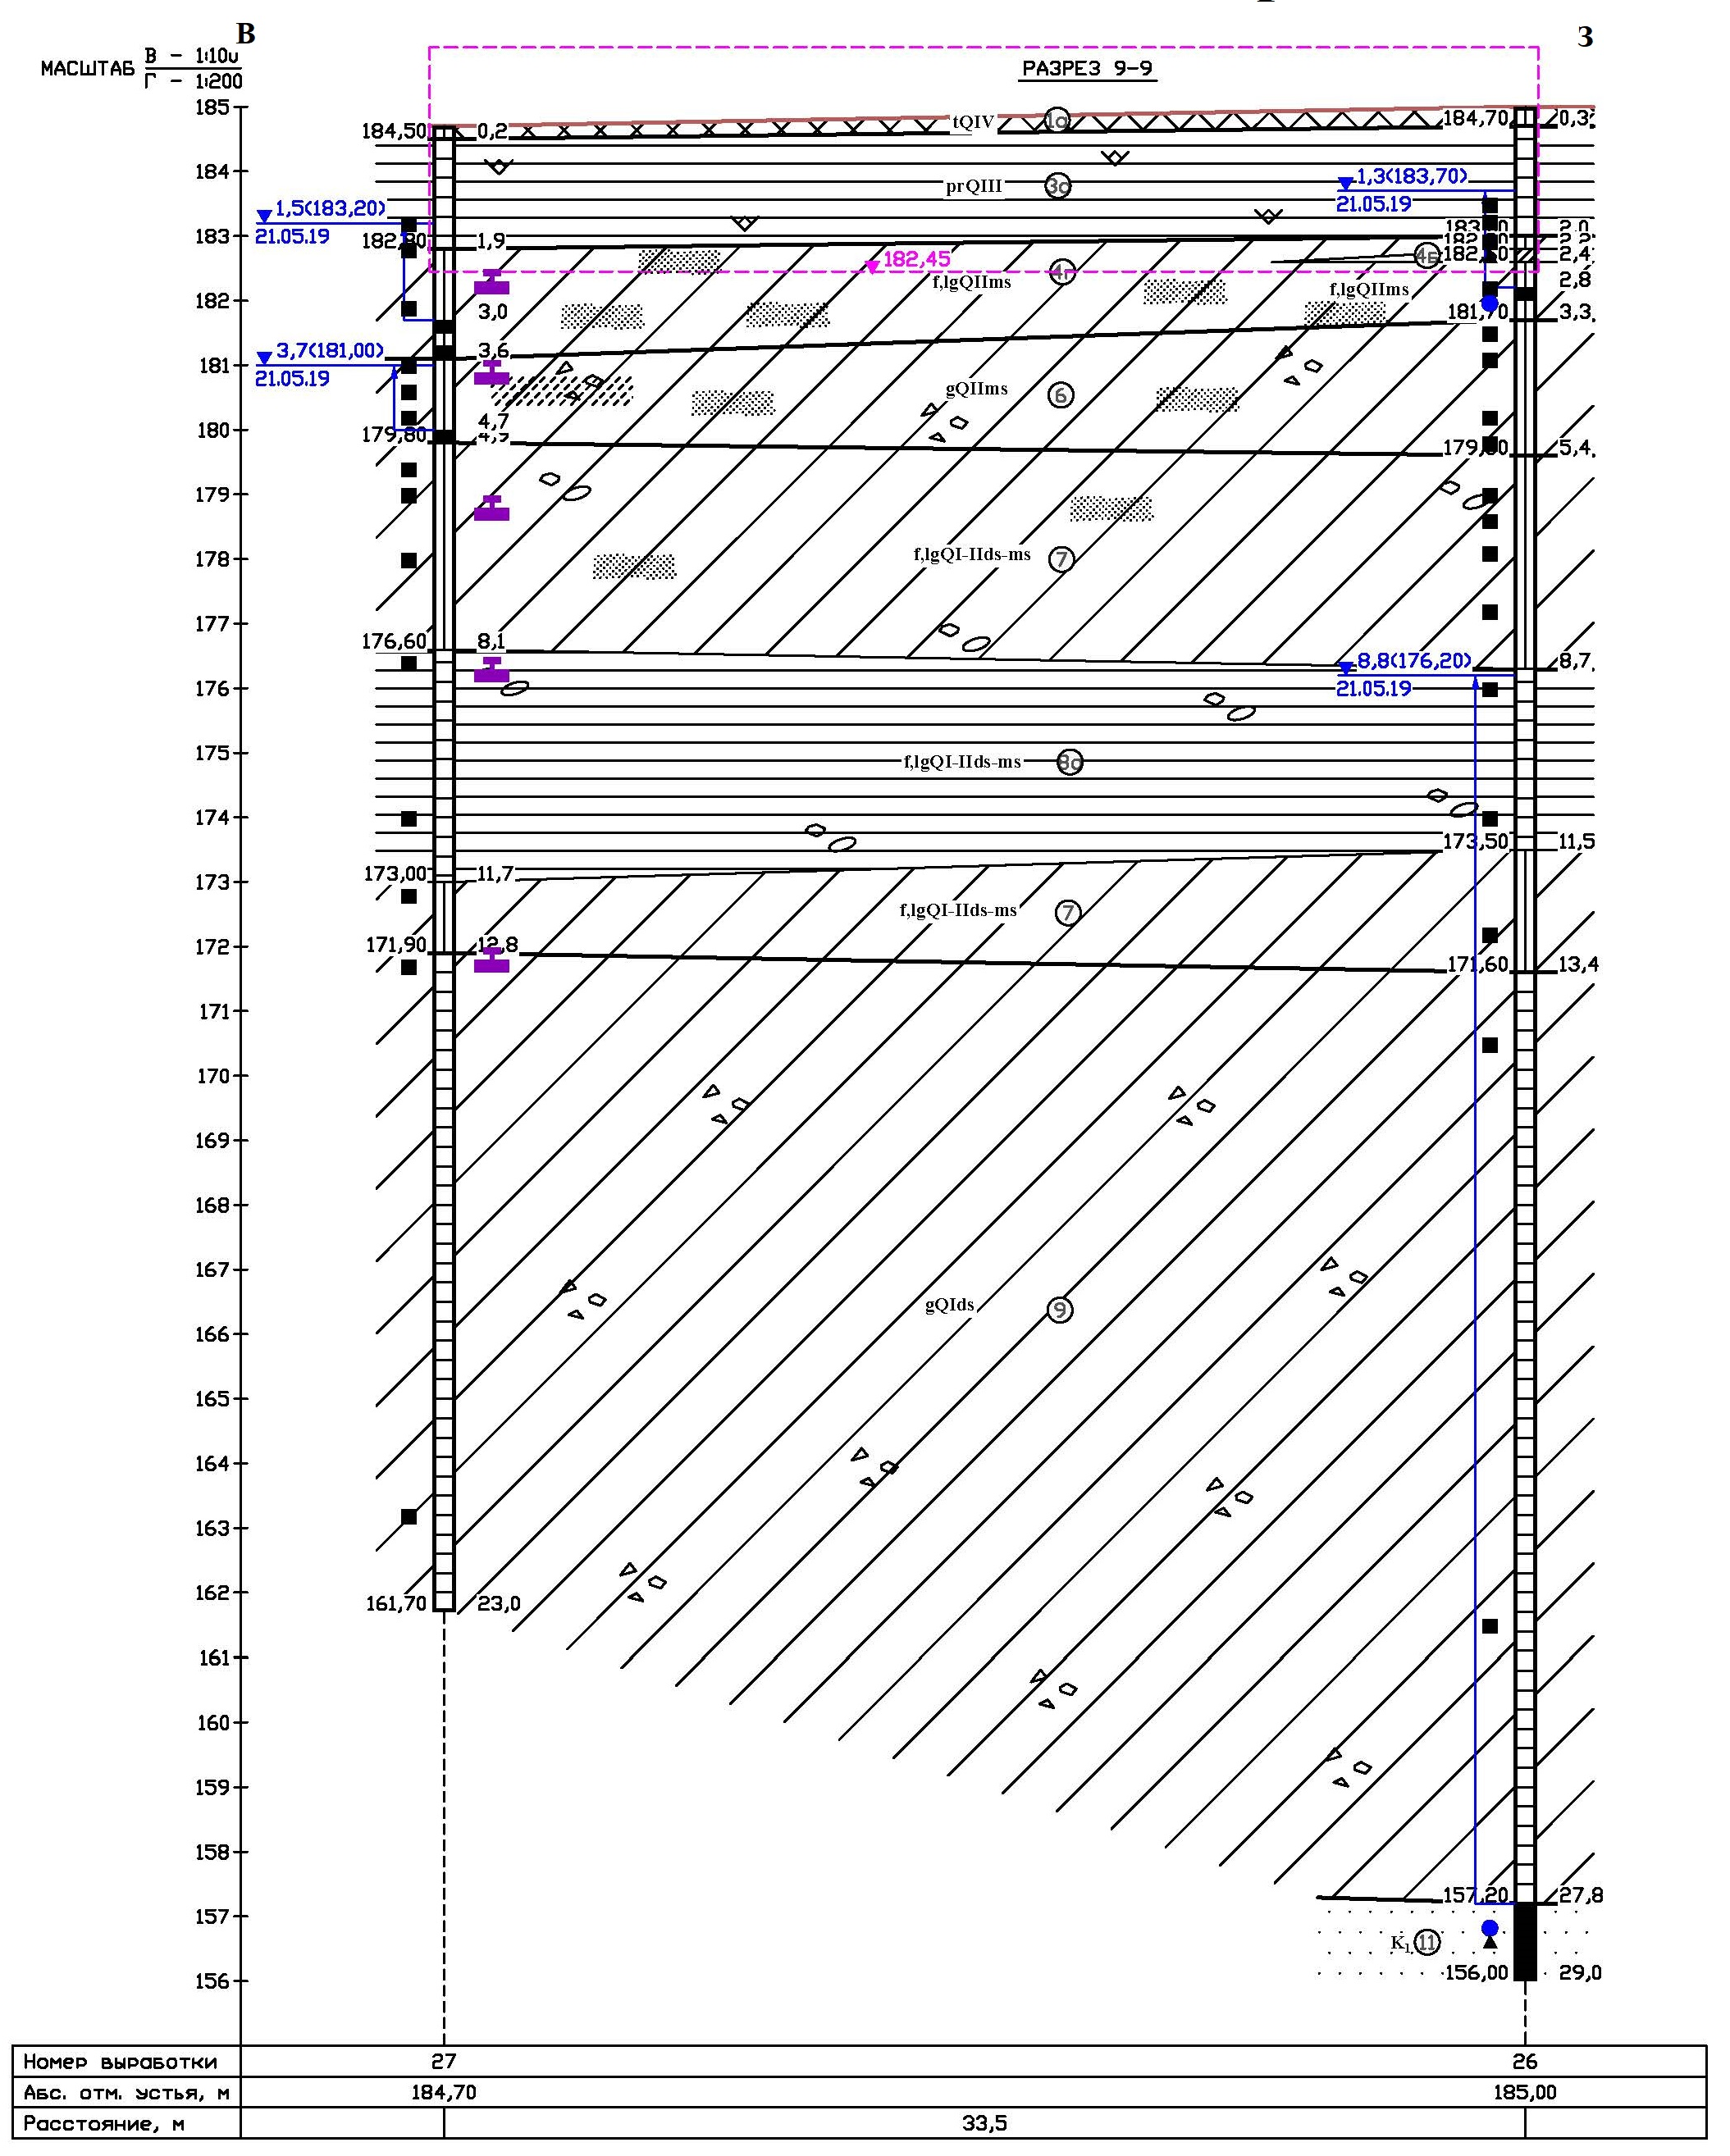
\includegraphics[scale=0.36]{images/razzr.png}
  }
  \caption{Инженерно-геологический разрез исследуемой территории (Технический отчет. Саларьево-парк, 2019)}\label{fig:fig}
\end{figure}

\begin{figure}[ht!]
  \centerfloat{
    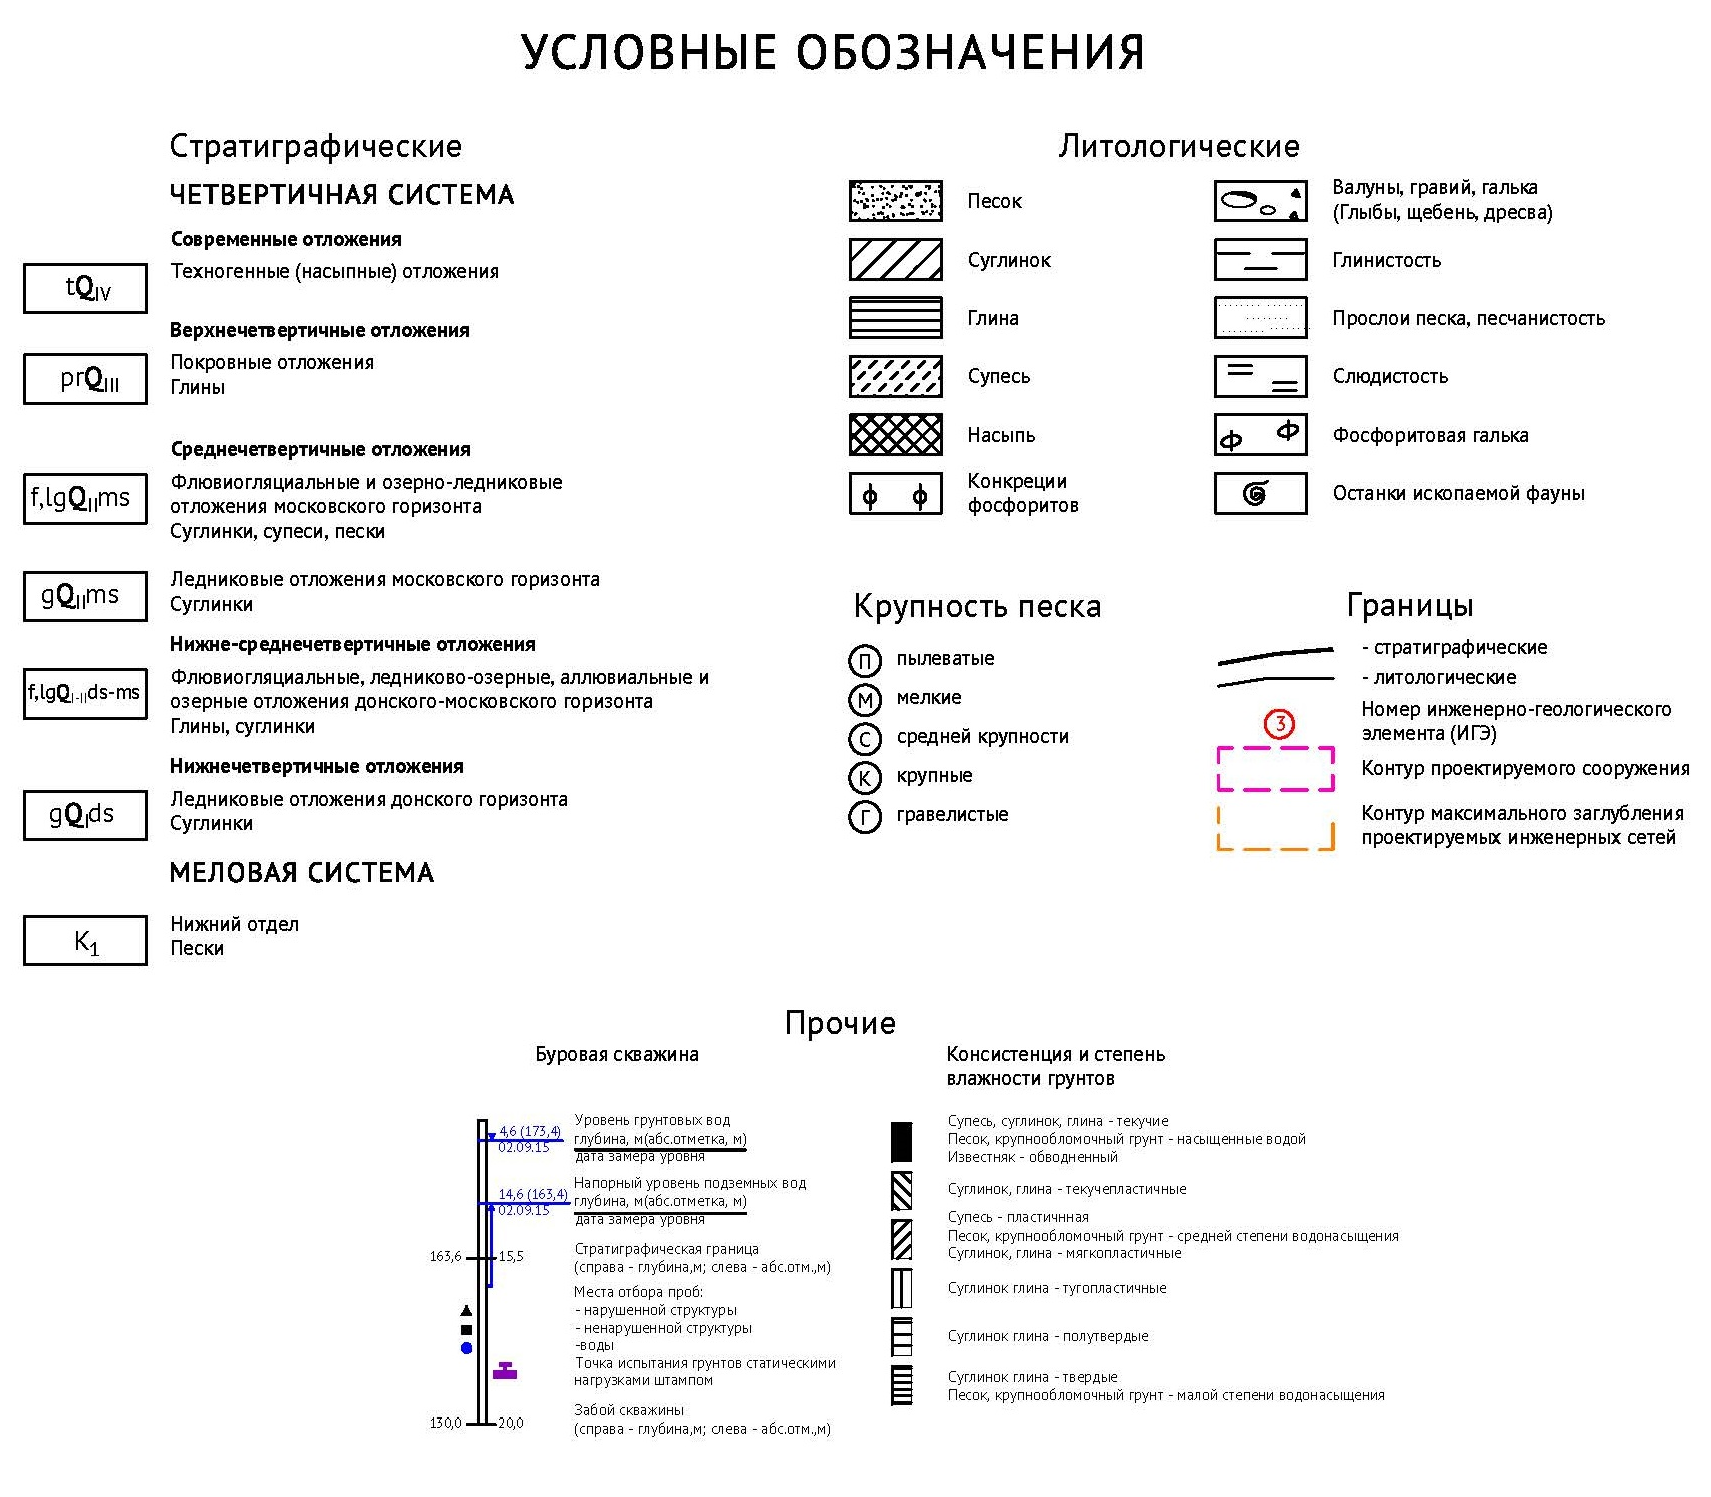
\includegraphics[scale=0.4]{images/usob.png}
  }
  \caption{Условные обозначения к инженерно-геологическому разрезу (Технический отчет. Саларьево-парк, 2019)}\label{fig:fig}
\end{figure}

 %\input{images/razrez.jpg}   
%\begin{sidewaysfigure}[ht]
%  \centerfloat{
%    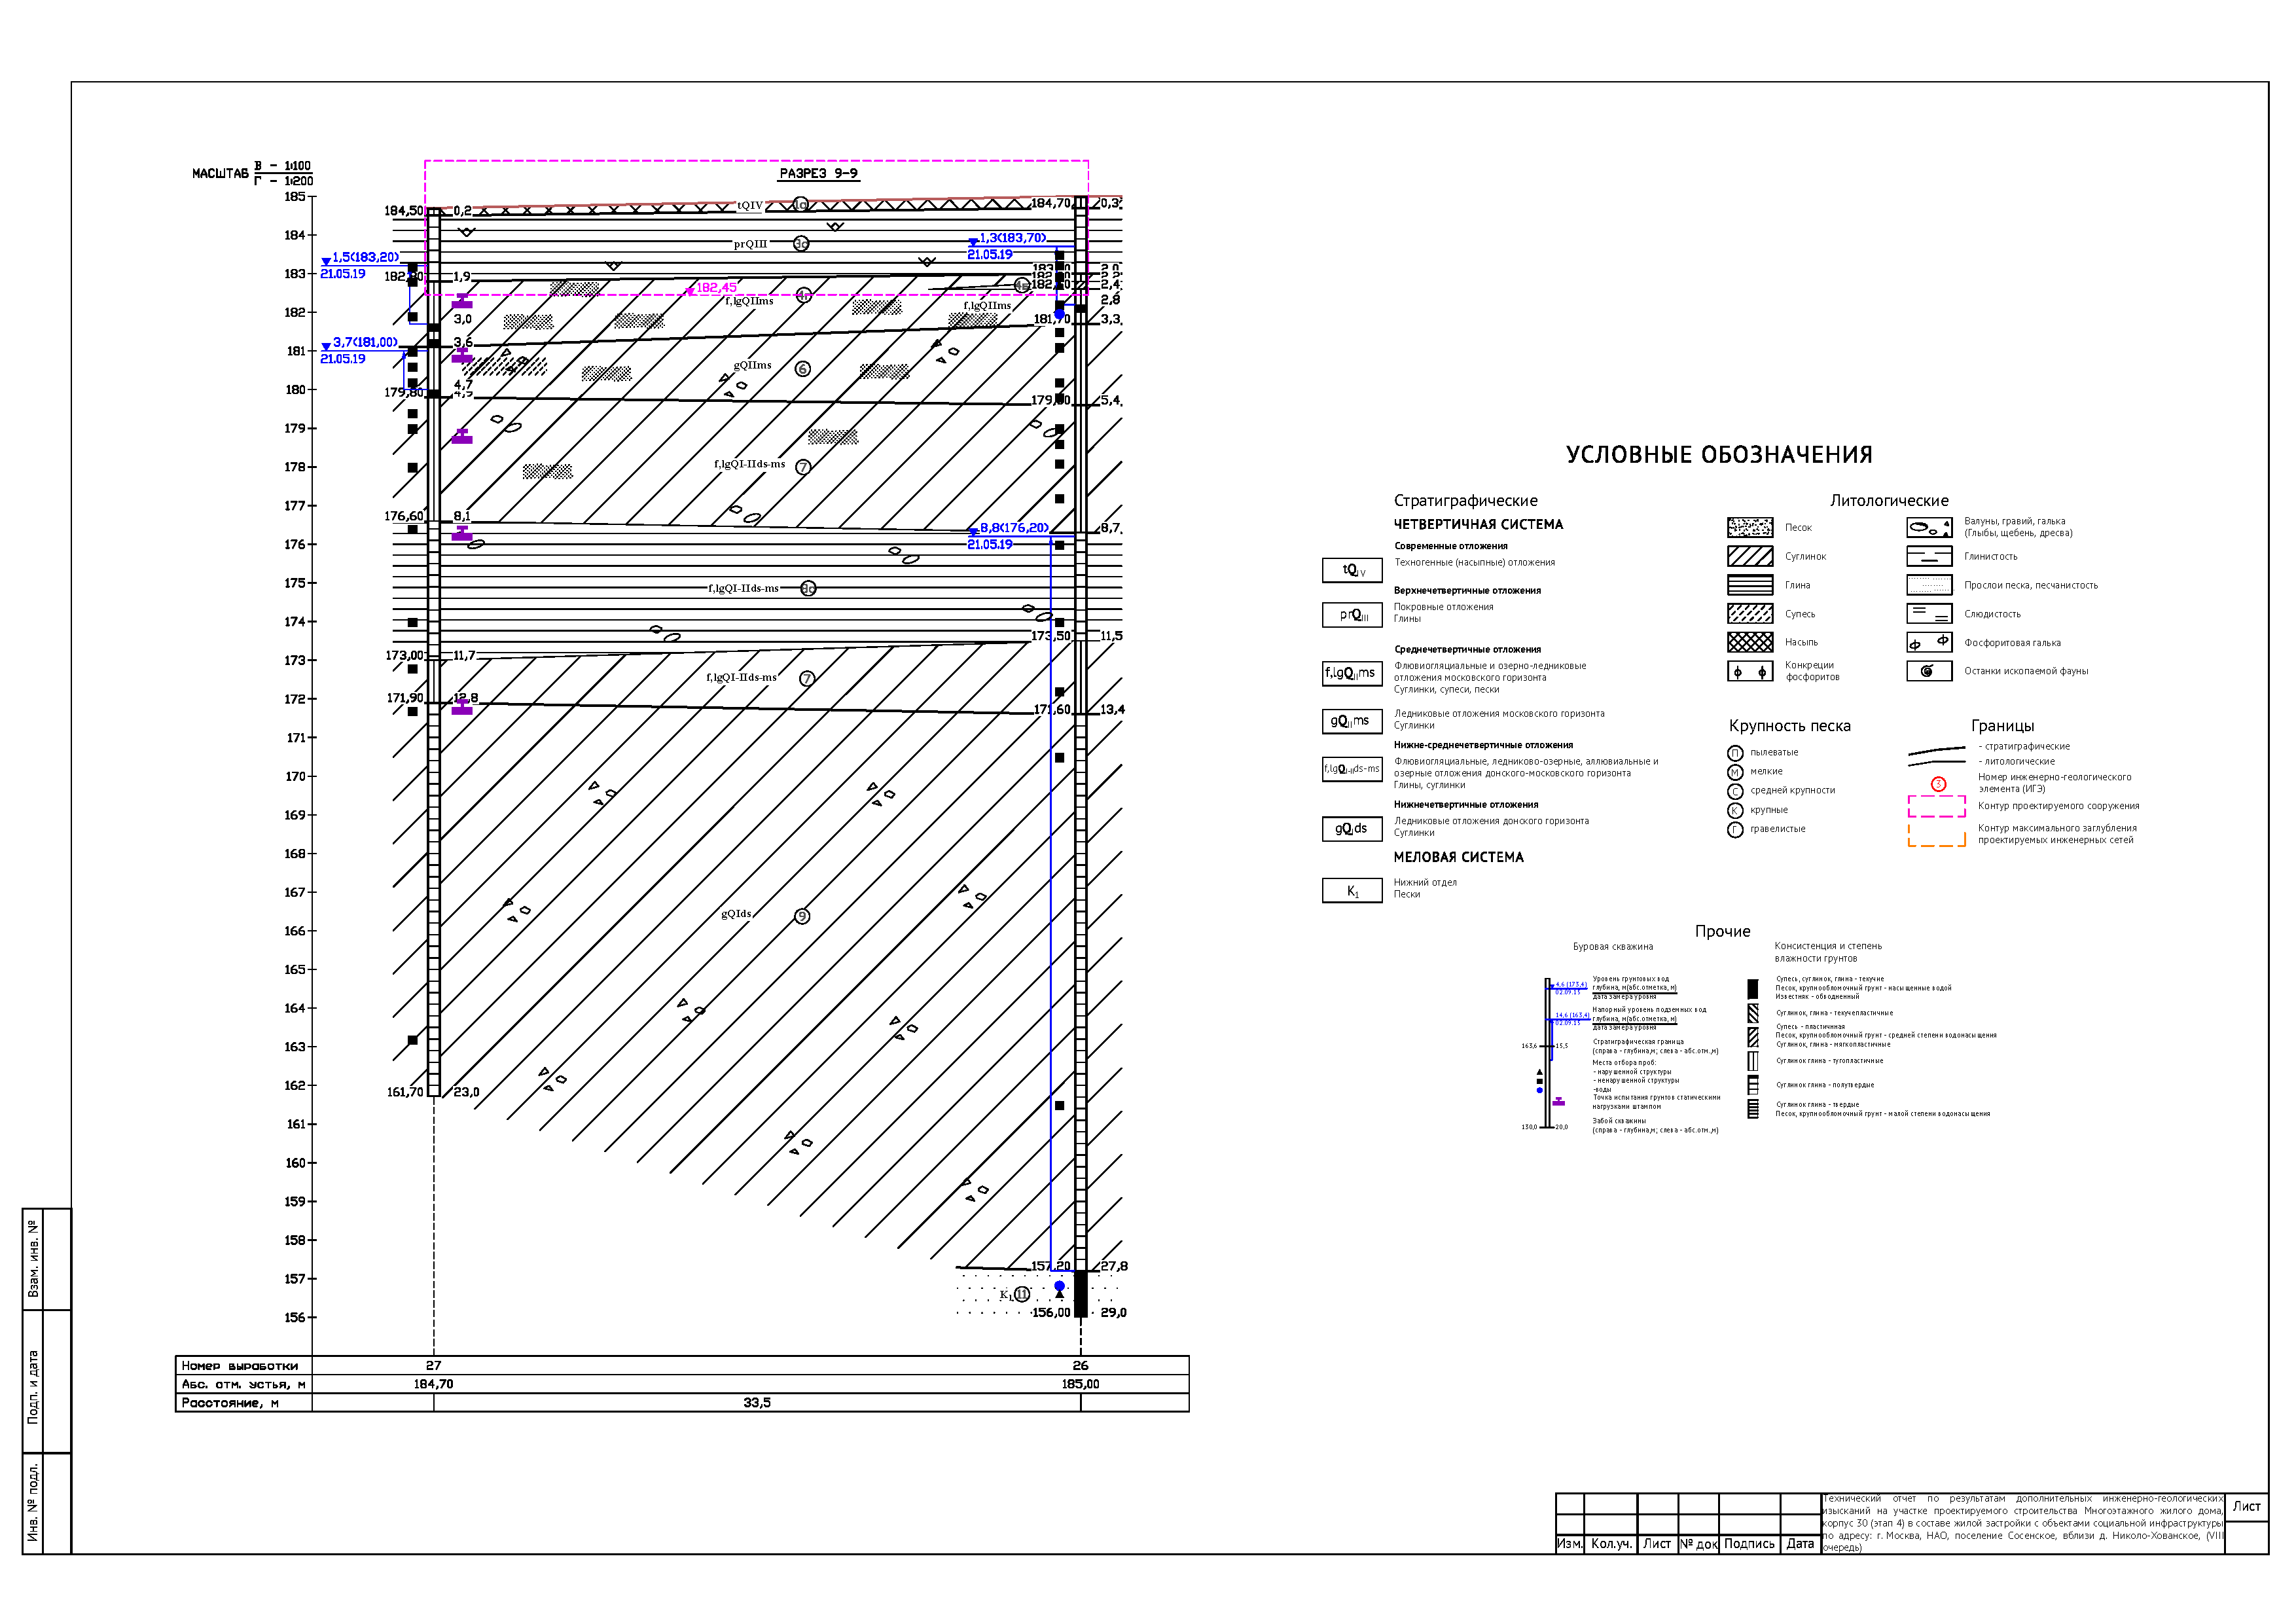
\includepdf[pages=-]{images/9-9.pdf}
%    \caption{Инженерно-геологический разрез}}
%\end{sidewaysfigure}


\begin{landscape}
\chapter{Физические свойства грунтов}\label{app:phisics}

%\begin{sidewaystable}[p]
   % \centering
   % \tiny
   % \caption{Физические свойства грунтов}
   % \begin{tabular}{@{}|l|r|r|r|r|r|r|r|r|r|r|p{4.8cm}|c|@{}}
   % \hline
   % Номер  & Глубина, \si{\meter} & $W$, д. е. & $W_l$, д. е. & $W_p$, д. е. & $I_p$ д .е & $I_l$, д.е. & $\rho$, г/\si{\centi\meter^3} & $\rho_s$, г/\si{\centi\meter^3} & $e$, д. е. & $S_r$, д. е. & Наименование   грунта                       & ИГЭ \\ \hline
   % GJ6805          & 3,5        & 0,171                        & 0,238   & 0,134  & 0,105  & 0,36     & 2,17     & 2,72      & 0,471   & 0,99     & суглинок легкий\linebreak   песчанистый тугопластичный & 6   \\ \hline
   % GJ6807          & 4,8        & 0,156                        & 0,228   & 0,129  & 0,099  & 0,27     & 2,17     & 2,69      & 0,449   & 0,95     & суглинок легкий\linebreak   песчанистый тугопластичный & 6   \\ \hline
   % GJ6838          & 4,3        & 0,150                        & 0,200   & 0,110  & 0,090  & 0,41     & 2,18     & 2,68      & 0,415   & 0,96     & суглинок легкий\linebreak  песчанистый тугопластичный & 6   \\\hline
   % GJ6835          & 3,5        & 0,150                        & 0,200   & 0,110  & 0,090  & 0,36     & 2,17     & 2,72      & 0,433   & 0,91     & суглинок легкий\linebreak   песчанистый тугопластичный & 6   \\ \hline
   % GJ6809          & 6,0        & 0,269                        & 0,322   & 0,210  & 0,112  & 0,53     & 1,97     & 2,72      & 0,752   & 0,97     & суглинок   мягкопластичный                   & 7   \\ \hline
   % GJ6810          & 6,4        & 0,251                        & 0,342   & 0,231  & 0,111  & 0,18     & 1,99     & 2,72      & 0,714   & 0,96     & суглинок полутвердый                         & 7   \\ \hline
   % GJ6821          & 6,7        & 0,233                        & 0,309   & 0,191  & 0,118  & 0,35     & 2,01     & 2,72      & 0,668   & 0,95     & суглинок   тугопластичный                    & 7   \\ \hline
   % GJ6898          & 12,1       & 0,240                        & 0,320   & 0,180  & 0,140  & 0,44     & 2,04     & 2,72      & 0,655   & 0,99     & суглинок тяжелый\linebreak   пылеватый тугопластичный  & 7   \\ \hline
   % GJ6874          & 7,4        & 0,240                        & 0,340   & 0,180  & 0,160  & 0,34     & 2,01     & 2,72      & 0,675   & 0,96     & суглинок тяжелый\linebreak   пылеватый тугопластичный  & 7   \\ \hline
   % GJ6888          & 10,2       & 0,230                        & 0,440   & 0,190  & 0,250  & 0,18     & 2,03     & 2,72      & 0,658   & 0,97     & глина легкая\linebreak   пылеватая полутвердая         & 8   \\ \hline
   % GJ6890          & 10,6       & 0,220                        & 0,410   & 0,170  & 0,230  & 0,18     & 2,07     & 2,72      & 0,602   & 0,98     & глина легкая\linebreak   песчанистая полутвердая       & 8   \\ \hline
   % GJ6852          & 10,3       & 0,210                        & 0,400   & 0,170  & 0,220  & 0,15     & 2,09     & 2,74      & 0,580   & 0,97     & глина полутвердая                            & 8   \\ \hline
   % GJ6889          & 10,4       & 0,220                        & 0,410   & 0,170  & 0,240  & 0,18     & 2,06     & 2,74      & 0,620   & 0,96     & глина полутвердая                            & 8   \\ \hline
   % GJ6822          & 8,3        & 0,244                        & 0,441   & 0,223  & 0,218  & 0,09     & 2,01     & 2,68      & 0,695   & 0,96     & глина полутвердая                            & 8   \\ \hline
   % GJ6884          & 9,2        & 0,220                        & 0,400   & 0,200  & 0,200  & 0,14     & 2,03     & 2,72      & 0,644   & 0,95     & глина легкая\linebreak   пылеватая полутвердая         & 8   \\ \hline
   % GJ6846          & 8,3        & 0,210                        & 0,510   & 0,210  & 0,310  & 0,02     & 2,08     & 2,72      & 0,585   & 0,99     & глина тяжелая\linebreak   полутвердая                  & 8   \\ \hline
   % GJ6855          & 11,7       & 0,192                        & 0,364   & 0,163  & 0,202  & 0,14     & 2,08     & 2,67      & 0,573   & 0,92     & глина легкая\linebreak   песчанистая полутвердая       & 9   \\ \hline
   % GJ6859          & 12,5       & 0,187                        & 0,374   & 0,166  & 0,208  & 0,1      & 2,10     & 2,72      & 0,549   & 0,93     & глина полутвердая                            & 9   \\ \hline
   % GJ6865          & 14,7       & 0,156                        & 0,312   & 0,134  & 0,179  & 0,12     & 2,18     & 2,72      & 0,442   & 0,94     & глина легкая\linebreak   песчанистая полутвердая       & 9   \\ \hline
   % GJ68A3          & 13,5       & 0,180                        & 0,330   & 0,150  & 0,180  & 0,18     & 2,10     & 2,68      & 0,509   & 0,95     & глина легкая\linebreak   песчанистая полутвердая       & 9   \\ \hline
   % GJ68B7          & 16,9       & 0,120                        & 0,300   & 0,130  & 0,170  & -0,06    & 2,26     & 2,72      & 0,354   & 0,94     & глина легкая       & 9   \\ \hline
   % GJ68A7          & 14,6       & 0,130                        & 0,290   & 0,140  & 0,160  & 0,08     & 2,23     & 2,72      & 0,372   & 0,91     & глина легкая                              & 9   \\ \hline
   % GJ6856          & 11,9       & 0,210                        & 0,380   & 0,160  & 0,210  & 0,22     & 2,09     & 2,74      & 0,588   & 0,97     & глина полутвердая                            & 9   \\ \hline
   % GJ68A0          & 12,6       & 0,180                        & 0,320   & 0,140  & 0,180  & 0,00     & 2,13     & 2,71      & 0,499   & 0,98     & глина легкая\linebreak   песчанистая полутвердая       & 9   \\ \hline
   % GJ6864          & 14,3       & 0,150                        & 0,310   & 0,140  & 0,170  & 0,06     & 2,19     & 2,72      & 0,433   & 0,97     & глина легкая \linebreak  песчанистая полутвердая       & 9   \\ \hline
   % \bottomrule 
   % \end{tabular}
   % \end{sidewaystable}

    \begin{table}[h]
      \small
      \centering
      \tiny
      \caption{Физические свойства грунтов}
      \begin{tabular}{@{}|l|r|r|r|r|r|r|r|r|r|r|r|@{}}
      \hline
      Номер  & Глубина, \si{\meter} & $W$, д. е. & $W_l$, д. е. & $W_p$, д. е. & $I_p$ д .е & $I_l$, д.е. & $\rho$, г/\si{\centi\meter^3} & $\rho_s$, г/\si{\centi\meter^3} & $e$, д. е. & $S_r$, д. е. & Наименование   грунта, ИГЭ \\ \hline
      GJ6805          & 3,5        & 0,171                        & 0,238   & 0,134  & 0,105  & 0,36     & 2,17     & 2,72      & 0,471   & 0,99     & суглинок легкий  тугопластичный, 6   \\ \hline
      GJ6807          & 4,8        & 0,156                        & 0,228   & 0,129  & 0,099  & 0,27     & 2,17     & 2,69      & 0,449   & 0,95     & суглинок легкий   тугопластичный, 6   \\ \hline
      GJ6838          & 4,3        & 0,150                        & 0,200   & 0,110  & 0,090  & 0,41     & 2,18     & 2,68      & 0,415   & 0,96     & суглинок легкий   тугопластичный, 6   \\\hline
      GJ6835          & 3,5        & 0,150                        & 0,200   & 0,110  & 0,090  & 0,36     & 2,17     & 2,72      & 0,433   & 0,91     & суглинок легкий   тугопластичный, 6   \\ \hline
      GJ6809          & 6,0        & 0,269                        & 0,322   & 0,210  & 0,112  & 0,53     & 1,97     & 2,72      & 0,752   & 0,97     & суглинок   мягкопластичный, 7   \\ \hline
      GJ6810          & 6,4        & 0,251                        & 0,342   & 0,231  & 0,111  & 0,18     & 1,99     & 2,72      & 0,714   & 0,96     & суглинок    полутвердый, 7   \\ \hline
      GJ6821          & 6,7        & 0,233                        & 0,309   & 0,191  & 0,118  & 0,35     & 2,01     & 2,72      & 0,668   & 0,95     & суглинок   тугопластичный, 7   \\ \hline
      GJ6898          & 12,1       & 0,240                        & 0,320   & 0,180  & 0,140  & 0,44     & 2,04     & 2,72      & 0,655   & 0,99     & суглинок тяжелый   тугопластичный, 7   \\ \hline
      GJ6874          & 7,4        & 0,240                        & 0,340   & 0,180  & 0,160  & 0,34     & 2,01     & 2,72      & 0,675   & 0,96     & суглинок тяжелый   тугопластичный, 7   \\ \hline
      GJ6888          & 10,2       & 0,230                        & 0,440   & 0,190  & 0,250  & 0,18     & 2,03     & 2,72      & 0,658   & 0,97     & глина легкая    полутвердая, 8   \\ \hline
      GJ6890          & 10,6       & 0,220                        & 0,410   & 0,170  & 0,230  & 0,18     & 2,07     & 2,72      & 0,602   & 0,98     & глина легкая    полутвердая, 8   \\ \hline
      GJ6852          & 10,3       & 0,210                        & 0,400   & 0,170  & 0,220  & 0,15     & 2,09     & 2,74      & 0,580   & 0,97     & глина полутвердая, 8   \\ \hline
      GJ6889          & 10,4       & 0,220                        & 0,410   & 0,170  & 0,240  & 0,18     & 2,06     & 2,74      & 0,620   & 0,96     & глина полутвердая, 8   \\ \hline
      GJ6822          & 8,3        & 0,244                        & 0,441   & 0,223  & 0,218  & 0,09     & 2,01     & 2,68      & 0,695   & 0,96     & глина полутвердая, 8   \\ \hline
      GJ6884          & 9,2        & 0,220                        & 0,400   & 0,200  & 0,200  & 0,14     & 2,03     & 2,72      & 0,644   & 0,95     & глина легкая    полутвердая, 8   \\ \hline
      GJ6846          & 8,3        & 0,210                        & 0,510   & 0,210  & 0,310  & 0,02     & 2,08     & 2,72      & 0,585   & 0,99     & глина тяжелая   полутвердая, 8   \\ \hline
      GJ6855          & 11,7       & 0,192                        & 0,364   & 0,163  & 0,202  & 0,14     & 2,08     & 2,67      & 0,573   & 0,92     & глина легкая    полутвердая, 9   \\ \hline
      GJ6859          & 12,5       & 0,187                        & 0,374   & 0,166  & 0,208  & 0,1      & 2,10     & 2,72      & 0,549   & 0,93     & глина полутвердая, 9   \\ \hline
      GJ6865          & 14,7       & 0,156                        & 0,312   & 0,134  & 0,179  & 0,12     & 2,18     & 2,72      & 0,442   & 0,94     & глина легкая    полутвердая, 9   \\ \hline
      GJ68A3          & 13,5       & 0,180                        & 0,330   & 0,150  & 0,180  & 0,18     & 2,10     & 2,68      & 0,509   & 0,95     & глина легкая    полутвердая, 9   \\ \hline
      GJ68B7          & 16,9       & 0,120                        & 0,300   & 0,130  & 0,170  & -0,06    & 2,26     & 2,72      & 0,354   & 0,94     & глина легкая, 9   \\ \hline
      GJ68A7          & 14,6       & 0,130                        & 0,290   & 0,140  & 0,160  & 0,08     & 2,23     & 2,72      & 0,372   & 0,91     & глина легкая, 9   \\ \hline
      GJ6856          & 11,9       & 0,210                        & 0,380   & 0,160  & 0,210  & 0,22     & 2,09     & 2,74      & 0,588   & 0,97     & глина полутвердая, 9   \\ \hline
      GJ68A0          & 12,6       & 0,180                        & 0,320   & 0,140  & 0,180  & 0,00     & 2,13     & 2,71      & 0,499   & 0,98     & глина легкая    полутвердая, 9   \\ \hline
      GJ6864          & 14,3       & 0,150                        & 0,310   & 0,140  & 0,170  & 0,06     & 2,19     & 2,72      & 0,433   & 0,97     & глина легкая    полутвердая, 9   \\ \hline
      \bottomrule 
      \end{tabular}
      \end{table}
    \end{landscape}

\chapter{Результаты рентгеноструктурного анализа}\label{app:difrac}
(инж. 1 кат. С.А. Гаранина, вед. инж. С.В. Закусин, ст.н.с. В.В. Крупская)

\begin{figure}[ht]
    \centerfloat{
      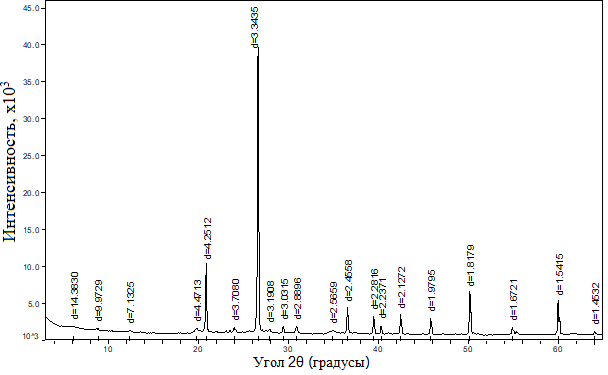
\includegraphics[scale=1.05]{dif68B7.png}
    }
    \caption{Рентгеновская дифракционная картина образца GJ68B7 (ИГЭ-9, суглинки полутвердые)}\label{fig:fig}
  \end{figure}

  \begin{figure}[ht]
    \centerfloat{
      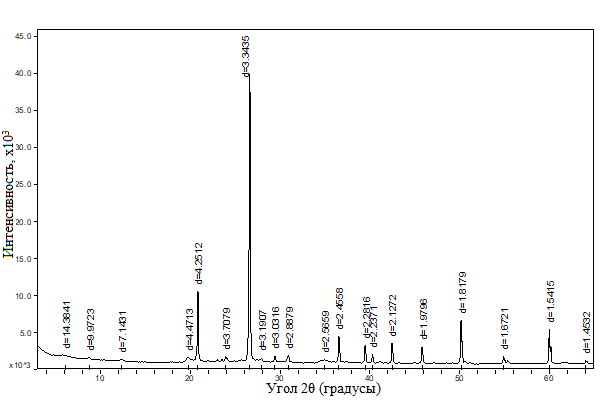
\includegraphics[scale=1.05]{dif68D4.png}
    }
    \caption{Рентгеновская дифракционная картина образца GJ68D4 (ИГЭ-9, суглинки полутвердые)}\label{fig:fig}
  \end{figure}

  \begin{figure}[ht]
    \centerfloat{
      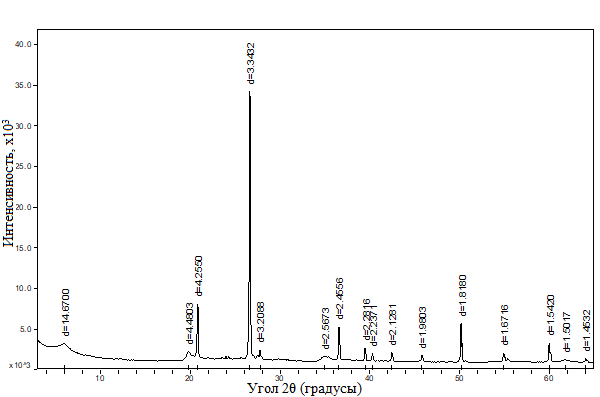
\includegraphics[scale=1.1]{dif6890.png}
    }
    \caption{Рентгеновская дифракционная картина образца GJ6890 (ИГЭ-8а, глины полутвердые)}\label{fig:fig}
  \end{figure}

  \begin{figure}[ht]
    \centerfloat{
      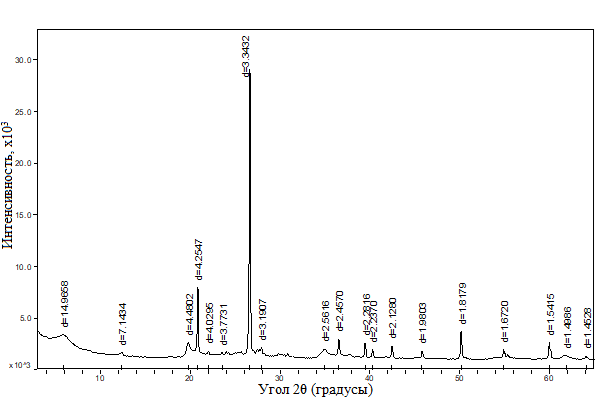
\includegraphics[scale=1.1]{dif6881.png}
    }
    \caption{Рентгеновская дифракционная картина образца GJ6881 (ИГЭ-8а, глины полутвердые)}\label{fig:fig}
  \end{figure}

  \begin{figure}[ht]
    \centerfloat{
      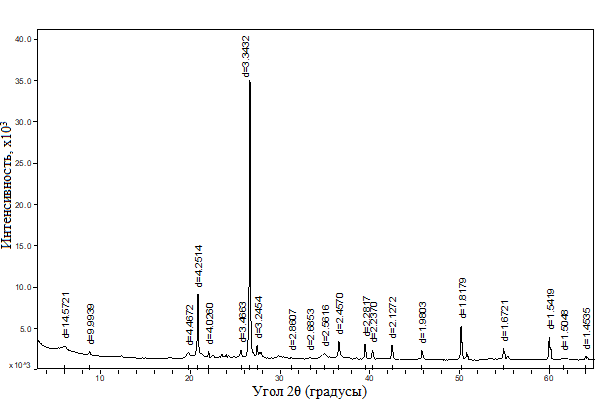
\includegraphics[scale=1.1]{dif6898.png}
    }
    \caption{Рентгеновская дифракционная картина образца GJ6898 (ИГЭ-7, суглинки тугопластичные)}\label{fig:fig}
  \end{figure}

  \begin{figure}[ht]
    \centerfloat{
      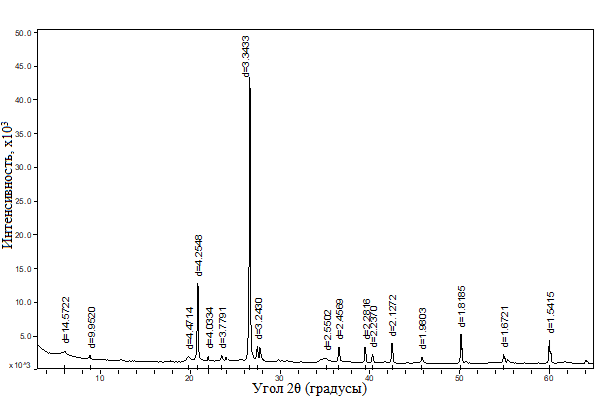
\includegraphics[scale=1.1]{dif6899.png}
    }
    \caption{Рентгеновская дифракционная картина образца GJ6899 (ИГЭ-7, суглинки тугопластичные)}\label{fig:fig}
  \end{figure}

\chapter{Компрессионные кривые}\label{app:oedometer}
\small
\pgfplotsset{
    % discard if not/.style 2 args={
    %     x filter/.code={
    %         \edef\tempa{\thisrow{#1}}
    %         \edef\tempb{#2}
    %         \ifx\tempa\tempb
    %         \else
    %             \def\pgfmathresult{inf}
    %         \fi
    %     }
    % }
}

\pgfplotsset{
% 	%samples=15,
	width= 0.9\linewidth,
	height = 10cm,
	xlabel={Вертикальное эфф. напряжение $\\sigma_1$, кПа},
	ylabel={Отн. верт. деформация $\epsilon_1$, д. е.},
% 	%extra y ticks={45},
	legend pos=north west,
	y dir=reverse, 
	y tick label style={
		/pgf/number format/.cd,
			fixed,
			fixed zerofill,
			precision=3,
		/tikz/.cd
	},
	ylabel near ticks,
	% ylabel shift = 5cm,
% 	% clip mode=individual,
	x tick label style={
        /pgf/number format/set thousands separator={\,},
		/pgf/number format/.cd,
			fixed,
			fixed zerofill
        /tikz/.cd
	},
    xticklabel={
        \pgfkeys{ /pgf/number format/fixed, 
            /pgf/number format/fixed zerofill, 
            /pgf/number format/precision=0} 
        \pgfmathparse{exp(\tick)}
        \pgfmathprintnumber{\pgfmathresult}
    }
}

{
\tiny

\begin{figure}[ht]
	\begin{tikzpicture}
		% \centering
		\begin{semilogxaxis}
		\addplot[mark=*, red] table [x=Sigma, y=Epsilon, col sep=semicolon] {data/GJ6805.csv};
		\end{semilogxaxis}
	\end{tikzpicture}
	\caption{Компрессионная кривая образца \texttt{GJ6805}}
\end{figure}

\begin{figure}
\begin{tikzpicture}
	\begin{semilogxaxis}[y dir=reverse]
	\addplot[mark=*, red] table [x=Sigma, y=Epsilon, col sep=semicolon] {data/GJ6807.csv};
	\end{semilogxaxis}
\end{tikzpicture}
\caption{\texttt{GJ6807}}
\end{figure}

\begin{figure}
\begin{tikzpicture}
	\begin{semilogxaxis}[y dir=reverse]
	\addplot[mark=*, red] table [x=Sigma, y=Epsilon, col sep=semicolon] {data/GJ6838.csv};
	\end{semilogxaxis}
\end{tikzpicture}
\caption{Компрессионная кривая образца \texttt{GJ6838}}
\end{figure}

\begin{figure}
\begin{tikzpicture}
	\begin{semilogxaxis}[y dir=reverse]
	\addplot[mark=*, red] table [x=Sigma, y=Epsilon, col sep=semicolon] {data/GJ6809.csv};
	\end{semilogxaxis}
\end{tikzpicture}
\caption{Компрессионная кривая образца \texttt{GJ6809}}
\end{figure}

\begin{figure}

\begin{tikzpicture}
	\begin{semilogxaxis}[y dir=reverse]
	\addplot[mark=*, red] table [x=Sigma, y=Epsilon, col sep=semicolon] {data/GJ6810.csv};
	\end{semilogxaxis}
\end{tikzpicture}
\caption{Компрессионная кривая образца \texttt{GJ6810}}
\end{figure}

\begin{figure}
\begin{tikzpicture}
	\begin{semilogxaxis}[y dir=reverse]
	\addplot[mark=*, red] table [x=Sigma, y=Epsilon, col sep=semicolon] {data/GJ6821.csv};
	\end{semilogxaxis}
\end{tikzpicture}
\caption{Компрессионная кривая образца \texttt{GJ6821}}
\end{figure}

\begin{figure}
\begin{tikzpicture}
	\begin{semilogxaxis}[y dir=reverse]
	\addplot[mark=*, red] table [x=Sigma, y=Epsilon, col sep=semicolon] {data/GJ6898.csv};
	\end{semilogxaxis}
\end{tikzpicture}
\caption{\texttt{GJ6898}}
\end{figure}

\begin{figure}
\begin{tikzpicture}
	\begin{semilogxaxis}[y dir=reverse]
	\addplot[mark=*, red] table [x=Sigma, y=Epsilon, col sep=semicolon] {data/GJ6822.csv};
	\end{semilogxaxis}
\end{tikzpicture}
\caption{Компрессионная кривая образца \texttt{GJ6822}}
\end{figure}

\begin{figure}
\begin{tikzpicture}
	\begin{semilogxaxis}[y dir=reverse]
	\addplot[mark=*, red] table [x=Sigma, y=Epsilon, col sep=semicolon] {data/GJ6884.csv};
	\end{semilogxaxis}
\end{tikzpicture}
\caption{Компрессионная кривая образца \texttt{GJ6884}}
\end{figure}

\begin{figure}
\begin{tikzpicture}
	\begin{semilogxaxis}[y dir=reverse]
	\addplot[mark=*, red] table [x=Sigma, y=Epsilon, col sep=semicolon] {data/GJ6846.csv};
	\end{semilogxaxis}§
\end{tikzpicture}
\caption{Компрессионная кривая образца \texttt{GJ6846}}
\end{figure}

\begin{figure}
\begin{tikzpicture}
	\begin{semilogxaxis}[y dir=reverse]
	\addplot[mark=*, red] table [x=Sigma, y=Epsilon, col sep=semicolon] {data/GJ6855.csv};
	\end{semilogxaxis}
\end{tikzpicture}
\caption{Компрессионная кривая образца \texttt{GJ6855}}
\end{figure}

\begin{figure}
\begin{tikzpicture}
	\begin{semilogxaxis}[y dir=reverse]
	\addplot[mark=*, red] table [x=Sigma, y=Epsilon, col sep=semicolon] {data/GJ6859.csv};
	\end{semilogxaxis}
\end{tikzpicture}
\caption{Компрессионная кривая образца \texttt{GJ6859}}
\end{figure}


\begin{figure}
\begin{tikzpicture}
	\begin{semilogxaxis}[y dir=reverse]
	\addplot[mark=*, red] table [x=Sigma, y=Epsilon, col sep=semicolon] {data/GJ6865.csv};
	\end{semilogxaxis}
\end{tikzpicture}
\caption{Компрессионная кривая образца \texttt{GJ6865}}
\end{figure}

	
\begin{figure}
\begin{tikzpicture}
	\begin{semilogxaxis}[y dir=reverse]
	\addplot[mark=*, red] table [x=Sigma, y=Epsilon, col sep=semicolon] {data/GJ68A3.csv};
	\end{semilogxaxis}
\end{tikzpicture}
\caption{Компрессионная кривая образца \texttt{GJ68A3}}
\end{figure}

	
\begin{figure}
\begin{tikzpicture}
	\begin{semilogxaxis}[y dir=reverse]
	\addplot[mark=*, red] table [x=Sigma, y=Epsilon, col sep=semicolon] {data/GJ68B7.csv};
	\end{semilogxaxis}
\end{tikzpicture}
\caption{Компрессионная кривая образца \texttt{GJ68B7}}
\end{figure}
}

\chapter{Построения для определения напряжения предуплотения}\label{app:method}
% Inkscape figure
\begin{figure}[h!]
    {\centering
      \def\svgwidth{11cm} % используем для изменения размера, если надо
      %\includesvg{figs/drawing}
      \small
      \subbottom[Метод Казагранде]{%
      \centering
      \input{images/oedometerCazagrande+monolith+1.pdf_tex} }
      \hfill 
      \\
      \hfill  
      \def\svgwidth{11cm}
      \subbottom[Метод Беккера]{%
      \centering
      \input{images/oedometerBecker+monolith+1.pdf_tex}}
      \hfill 
      }
      \caption{Определение напряжения предуплотнения образца \texttt{GJ6805} (ИГЭ-6, суглинки тугопластичные)}
      \label{img:6805}
    \end{figure}
    
    \begin{figure}
        {\centering
        \small
          %\def\svgwidth{5cm} % используем для изменения размера, если надо
          %\includesvg{figs/drawing}
          \subbottom[Метод Казагранде]{%
          \centering
          \input{images/oedometerCazagrande+monolith+2.pdf_tex} }
          \hfill 
          \\
          \hfill  
          \subbottom[Метод Беккера]{%
          \centering
          \input{images/oedometerBecker+monolith+2.pdf_tex}}
          \hfill 
          }
          \caption{Определение напряжения предуплотнения образца \texttt{GJ6807} (ИГЭ-6, суглинки тугопластичные)}
          \label{img:6807}
    \end{figure}
    
    \begin{figure}
        {\centering
        \small
            %\def\svgwidth{5cm} % используем для изменения размера, если надо
            %\includesvg{figs/drawing}
            \subbottom[Метод Казагранде]{%
            \centering
            \input{images/oedometerCazagrande+monolith+3.pdf_tex} }
            \hfill 
            \\
            \hfill  
            \subbottom[Метод Беккера]{%
            \centering
            \input{images/oedometerBecker+monolith+3.pdf_tex}}
            \hfill 
            }
            \caption{Определение напряжения предуплотнения образца \texttt{GJ6838} (ИГЭ-6, суглинки тугопластичные)}
            \label{img:6838}
    \end{figure}
    
    
    \begin{figure}
        {\centering
        \small
            %\def\svgwidth{5cm} % используем для изменения размера, если надо
            %\includesvg{figs/drawing}
            \subbottom[Метод Казагранде]{%
            \centering
            \input{images/oedometerCazagrande+monolith+4.pdf_tex} }
            \hfill 
            \\
            \hfill  
            \subbottom[Метод Беккера]{%
            \centering
            \input{images/oedometerBecker+monolith+4.pdf_tex}}
            \hfill 
            }
            \caption{Определение напряжения предуплотнения образца \texttt{GJ6809} (ИГЭ-7, суглинки тугопластичные)}
            \label{img:6809}
    \end{figure}
    
    \begin{figure}
        {\centering
        \small
            %\def\svgwidth{5cm} % используем для изменения размера, если надо
            %\includesvg{figs/drawing}
            \subbottom[Метод Казагранде]{%
            \centering
            \input{images/oedometerCazagrande+monolith+5.pdf_tex} }
            \hfill 
            \\
            \hfill  
            \subbottom[Метод Беккера]{%
            \centering
            \input{images/oedometerBecker+monolith+5.pdf_tex}}
            \hfill 
            }
            \caption{Определение напряжения предуплотнения образца \texttt{GJ6810} (ИГЭ-7, суглинки тугопластичные)}
            \label{img:6810}
    \end{figure}
    
    \begin{figure}
        {\centering
        \small
            %\def\svgwidth{5cm} % используем для изменения размера, если надо
            %\includesvg{figs/drawing}
            \subbottom[Метод Казагранде]{%
            \centering
            \input{images/oedometerCazagrande+monolith+6.pdf_tex} }
            \hfill 
            \\
            \hfill  
            \subbottom[Метод Беккера]{%
            \centering
            \input{images/oedometerBecker+monolith+6.pdf_tex}}
            \hfill 
            }
            \caption{Определение напряжения предуплотнения образца \texttt{GJ6821} (ИГЭ-7, суглинки тугопластичные)}
            \label{img:6821}
    \end{figure}
    
    \begin{figure}
        {\centering
        \small
            %\def\svgwidth{5cm} % используем для изменения размера, если надо
            %\includesvg{figs/drawing}
            \subbottom[Метод Казагранде]{%
            \centering
            \input{images/oedometerCazagrande+monolith+7.pdf_tex} }
            \hfill 
            \\
            \hfill  
            \subbottom[Метод Беккера]{%
            \centering
            \input{images/oedometerBecker+monolith+7.pdf_tex}}
            \hfill 
            }
            \caption{Определение напряжения предуплотнения образца \texttt{GJ6898} (ИГЭ-7, суглинки тугопластичные)}
            \label{img:6898}
    \end{figure}
    
    \begin{figure}
        {\centering
        \small
            %\def\svgwidth{5cm} % используем для изменения размера, если надо
            %\includesvg{figs/drawing}
            \subbottom[Метод Казагранде]{%
            \centering
            \input{images/oedometerCazagrande+monolith+8.pdf_tex} }
            \hfill 
            \\
            \hfill  
            \subbottom[Метод Беккера]{%
            \centering
            \input{images/oedometerBecker+monolith+8.pdf_tex}}
            \hfill 
            }
            \caption{Определение напряжения предуплотнения образца \texttt{GJ6822} (ИГЭ-8а, глины полутвердые)}
            \label{img:6822}
    \end{figure}
    
    \begin{figure}
        {\centering
        \small
            %\def\svgwidth{5cm} % используем для изменения размера, если надо
            %\includesvg{figs/drawing}
            \subbottom[Метод Казагранде]{%
            \centering
            \input{images/oedometerCazagrande+monolith+9.pdf_tex} }
            \hfill 
            \\
            \hfill  
            \subbottom[Метод Беккера]{%
            \centering
            \input{images/oedometerBecker+monolith+9.pdf_tex}}
            \hfill 
        }
        \caption{Определение напряжения предуплотнения образца \texttt{GJ6884} (ИГЭ-8а, глины полутвердые)}
        \label{img:6884}
    \end{figure}
    
    \begin{figure}
        {\centering
        \small
            %\def\svgwidth{5cm} % используем для изменения размера, если надо
            %\includesvg{figs/drawing}
            \subbottom[Метод Казагранде]{%
            \centering
            \input{images/oedometerCazagrande+monolith+10.pdf_tex} }
            \hfill 
            \\
            \hfill  
            \subbottom[Метод Беккера]{%
            \centering
            \input{images/oedometerBecker+monolith+10.pdf_tex}}
            \hfill  
            }
            \caption{Определение напряжения предуплотнения образца \texttt{GJ6846} (ИГЭ-8а, глины полутвердые)}
            \label{img:6846}
    \end{figure}
    
    \begin{figure}
        {\centering
            %\def\svgwidth{5cm} % используем для изменения размера, если надо
            %\includesvg{figs/drawing}
            \small
            \subbottom[Метод Казагранде]{%
            \centering
            \input{images/oedometerCazagrande+monolith+11.pdf_tex} }
            \hfill 
            \\
            \hfill  
            \subbottom[Метод Беккера]{%
            \centering
            \input{images/oedometerBecker+monolith+11.pdf_tex}}
            \hfill  
            }
            \caption{Определение напряжения предуплотнения образца \texttt{GJ6855} (ИГЭ-9, суглинки полутвердые)}
            \label{img:6855}
    \end{figure}
    
    \begin{figure}
        {\centering
            %\def\svgwidth{5cm} % используем для изменения размера, если надо
            %\includesvg{figs/drawing}
            \small
            %\hfill
            \subbottom[Метод Казагранде]{%
            \centering
            \input{images/oedometerCazagrande+monolith+12.pdf_tex} }
            \hfill 
            \\
            \hfill   
            \subbottom[Метод Беккера]{%
            \centering
            \input{images/oedometerBecker+monolith+12.pdf_tex}}
            \hfill 
            }
            \caption{Определение напряжения предуплотнения образца \texttt{GJ6859} (ИГЭ-9, суглинки полутвердые)}
            \label{img:6859}
    \end{figure}
        
    \begin{figure}
        {\centering
            %\def\svgwidth{5cm} % используем для изменения размера, если надо
            %\includesvg{figs/drawing}
            \small
            %\hfill
            \subbottom[Метод Казагранде]{%
            \centering
            \input{images/oedometerCazagrande+monolith+13.pdf_tex} }
            \hfill 
            \\
            \hfill   
            \subbottom[Метод Беккера]{%
            \centering
            \input{images/oedometerBecker+monolith+13.pdf_tex}}
            \hfill 
            }
            \caption{Определение напряжения предуплотнения образца \texttt{GJ6865} (ИГЭ-9, суглинки полутвердые)}
            \label{img:6865}
    \end{figure}
        
    \begin{figure}
        {\centering
            %\def\svgwidth{5cm} % используем для изменения размера, если надо
            %\includesvg{figs/drawing}
            \small
            %\hfill
            \subbottom[Метод Казагранде]{%
            \centering
            \input{images/oedometerCazagrande+monolith+14.pdf_tex} }
            \hfill 
            \\
            \hfill   
            \subbottom[Метод Беккера]{%
            \centering
            \input{images/oedometerBecker+monolith+14.pdf_tex}}
            \hfill 
            }
            \caption{Определение напряжения предуплотнения образца \texttt{GJ68A3} (ИГЭ-9, суглинки полутвердые)}
            \label{img:68A3}
    \end{figure}
        
    \begin{figure}
        {\centering
            %\def\svgwidth{5cm} % используем для изменения размера, если надо
            %\includesvg{figs/drawing}
            \small
            %\hfill
            \subbottom[Метод Казагранде]{%
            \centering
            \input{images/oedometerCazagrande+monolith+15.pdf_tex} }
            \hfill 
            \\
            \hfill   
            \subbottom[Метод Беккера]{%
            \centering
            \input{images/oedometerBecker+monolith+15.pdf_tex}}
            \hfill 
            }
            \caption{Определение напряжения предуплотнения образца \texttt{GJ68B7} (ИГЭ-9, суглинки полутвердые)}
            \label{img:68B7}
    \end{figure}        % Приложения

\end{document}
